%%    _____  _____
%%   |  __ \|  __ \    AUTHOR: Pedro Rivero
%%   | |__) | |__) |   ---------------------------------
%%   |  ___/|  _  /    DATE: November 10, 2021
%%   | |    | | \ \    ---------------------------------
%%   |_|    |_|  \_\   https://github.com/pedrorrivero
%%

% \documentclass[9pt, aspectratio=169]{beamer}
\documentclass[9pt, handout, aspectratio=169]{beamer}	% Skip \pause commands
\usetheme[iit, sectiontoc]{PRwide}
\usepackage{PRmath}

% \setbeameroption{show notes}
% \setbeameroption{show only notes}

%% ----------------------------------------------------------------------------
%% FRONT-MATTER
%% ----------------------------------------------------------------------------

\title{Quantum Computation for the Understanding of Mass}
\subtitle{Simulating Quantum Field Theories}
\author{Pedro Rivero}
\institute{Illinois Institute of Technology \\ Argonne National Laboratory}
\newcommand{\mail}{priveroramirez@hawk.iit.edu}
\date{\today}
\newcommand{\website}{
	\href{https://github.com/pedrorrivero}
	{github.com/pedrorrivero}
}

\begin{document}
	\justify
	\setlength{\abovedisplayskip}{0pt}
	\setlength{\belowdisplayskip}{12pt}
	\setlength{\abovedisplayshortskip}{0pt}
	\setlength{\belowdisplayshortskip}{12pt}

\begin{frame}[plain,t]
	\titlepage
\end{frame}

\begin{frame}
  \frametitle{Table of Contents}
  \begin{multicols}{2}
    \tableofcontents%[currentsection]
  \end{multicols}
\end{frame}


%% ----------------------------------------------------------------------------
%% MAIN-MATTER
%% ----------------------------------------------------------------------------

%%    _____  _____
%%   |  __ \|  __ \    AUTHOR: Pedro Rivero
%%   | |__) | |__) |   ---------------------------------
%%   |  ___/|  _  /    DATE: November 10, 2021
%%   | |    | | \ \    ---------------------------------
%%   |_|    |_|  \_\   https://github.com/pedrorrivero
%%

%% ----------------------------------------------------------------------------

\begin{frame}{Introduction}

	Nature is described through the mathematical framework provided by \textbf{Quantum Field Theory}.

	\begin{multicols}{2}

		\begin{itemize}
			\item<2-> The different implementations of Quantum Field Theory are referred to as quantum field theories themselves.
			\item<3-> Quantum Chromodynamics (QCD) is the theory of the strong nuclear force.
			\item<3-> QCD holds many mysteries (e.g. \textbf{mass generation} phenomena).
			\item<4-> Many aspects of quantum field theories cannot be studied using classical computers.
      \item<4-> Physicists seek alternative tractable models to study interesting aspects of QCD.
		\end{itemize}

		\begin{center}
			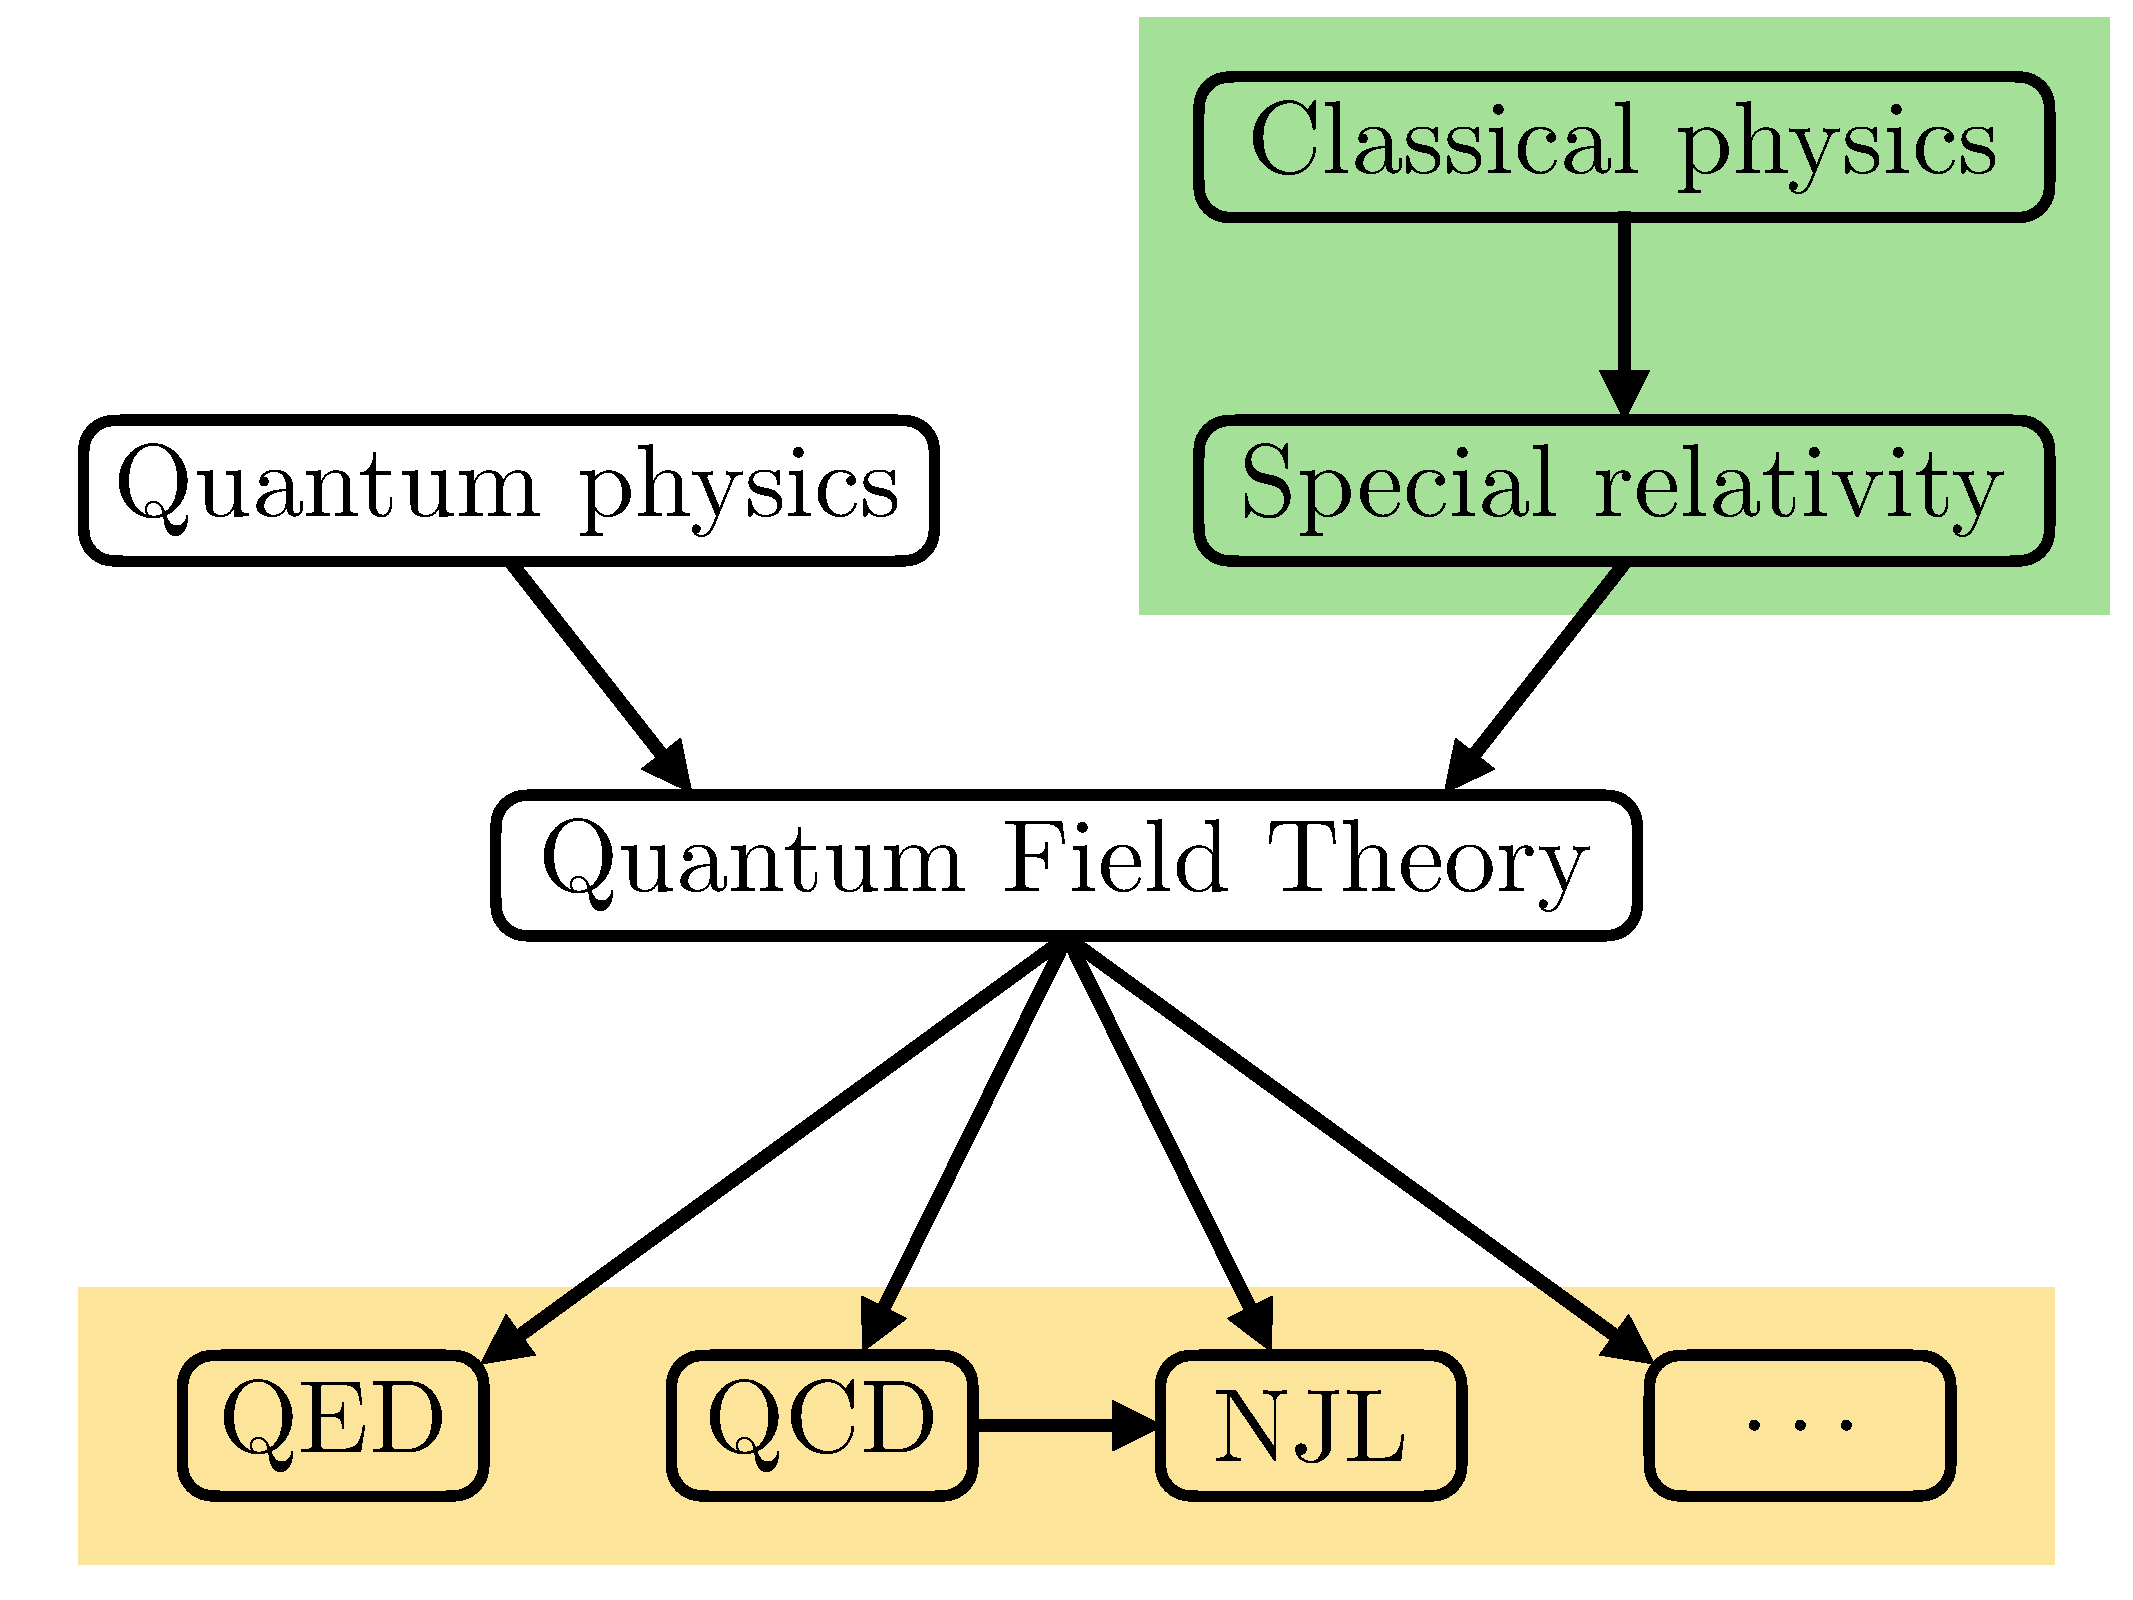
\includegraphics[width=.40\paperwidth]{Figures/quantum-field-theory}
		\end{center}

	\end{multicols}

\end{frame}

%% ----------------------------------------------------------------------------

% \begin{frame}{Objectives}
%
% 	An important path forward is to develop methods to simulate these models on quantum computers. This effort is only just beginning, however, performing calculations on a quantum computer is far from being a straightforward task; and it has only been achieved for relatively simple problems. My goal will be to develop some of the techniques necessary to use quantum computers for this endeavor. We will do so by analyzing the following:
%
% 	\medskip
%
% 	\begin{itemize}
% 		\item<2-> \textbf{Nambu--Jona-Lasino model} (NJL) in $1+1$ dimensions: an effective field theory, regarded as a low-energy approximation to QCD.
% 		\item<3-> It retains certain key features of QCD, such as the so called Goldstone modes and \textbf{dynamical chiral symmetry breaking}; which in turn is responsible for the creation of dressed mass.
% 		\item<4-> This model can be solved nonperturbatively through the standard leading order truncation; an important characteristic since verifying the solutions returned by any quantum computation is currently a major challenge.
% 	\end{itemize}
%
% \end{frame}

%%    _____  _____
%%   |  __ \|  __ \    AUTHOR: Pedro Rivero
%%   | |__) | |__) |   ---------------------------------
%%   |  ___/|  _  /    DATE: November 10, 2021
%%   | |    | | \ \    ---------------------------------
%%   |_|    |_|  \_\   https://github.com/pedrorrivero
%%

\section{The NJL model}

%% ----------------------------------------------------------------------------
%% ----------------------------------------------------------------------------

\begin{frame}[allowframebreaks]{The Nambu--Jona-Lasino model (NJL)}

	An important path forward is to develop methods to simulate these models on quantum computers. This effort is only just beginning, however, it has only been achieved for relatively simple problems.

	\medskip

	\begin{itemize}
		\item<2-> \textbf{Nambu--Jona-Lasino model} (NJL) in $1+1$ dimensions: an effective field theory, regarded as a low-energy approximation to QCD.
    \item<2-> Originally developed pre-QCD to describe nucleons via an effective two-body point interaction. Nowadays gets reinterpreted as a theory of quarks.
    \item<2-> Inspired by the \textbf{BCS theory of superconductivity}.
		\item<3-> It retains certain key features of QCD, such as the so called Goldstone modes and \textbf{dynamical chiral symmetry breaking}; which in turn is responsible for the creation of dressed mass.
		\item<4-> This model can be solved nonperturbatively through the standard leading order truncation; an important characteristic since verifying the solutions returned by any quantum computation is currently a major challenge.
	\end{itemize}

%% ----------------------------------------------------------------------------
\break
%% ----------------------------------------------------------------------------

	The NJL \textbf{Lagrangian density} that we will make use of looks like:

	\begin{gather*}
		\mathcal{L}(x) =
	    \bar{\psi}_{\alpha}(x)
	    \qty(\delta_{\alpha\beta}i\slashed{\partial}-\hat{m}_{\alpha\beta})
	    \psi_{\beta}(x) + \mathcal{L}_{I}(x) \\[1em]
		\mathcal{L}_{I}(x) =
	    \frac{1}{2} G_{\pi} \qty[\bar{\psi}_{\alpha}(x)\psi_{\alpha}(x)]^2
	\end{gather*}

	From this expression for the Lagrangian density we can obtain the corresponding \textbf{Hamiltonian density} through the Legendre transform. In special, for $1+1$ dimensions:

	\begin{align*}
		\mathcal{H} \,=\,\,
	  & -\frac{i}{2} \bar{\psi}_{\alpha} \gamma^{1}
	    \qty(\partial_{1} \psi_{\alpha}) +
	    \frac{i}{2} \qty(\partial_{1}\bar{\psi}_{\alpha})\gamma^{1}\psi_{\alpha} +
	    \bar{\psi}_{\alpha} \hat{m}_{\alpha\beta} \psi_{\beta} -
	    \frac{1}{2} G_{\pi} \qty(\bar{\psi}_{\alpha}\psi_{\alpha})^{2}
	\end{align*}

\end{frame}


%% ----------------------------------------------------------------------------
%% ANALYTICAL SOLUTION
%% ----------------------------------------------------------------------------

\subsection{Analytical solution}

%% ----------------------------------------------------------------------------
%% ----------------------------------------------------------------------------

\begin{frame}[allowframebreaks]{Dressed mass and the gap equation}

  \vspace{-1em}
	\begin{multicols}{2}

		The \textbf{bare and dressed masses} appear on the bare quark propagator $S_{0}$, and the NJL dressed quark propagator $S$ respectively:

		\vspace{1em}

		\begin{gather*}
		  S_0^{-1} \defeq \slashed{p} - m + i\varepsilon \\[.5em]
		  S^{-1} \equiv S^{-1}_\text{\tiny NJL} \defeq \slashed{p} - M + i\varepsilon
		\end{gather*}

		\columnbreak

		\begin{center}
			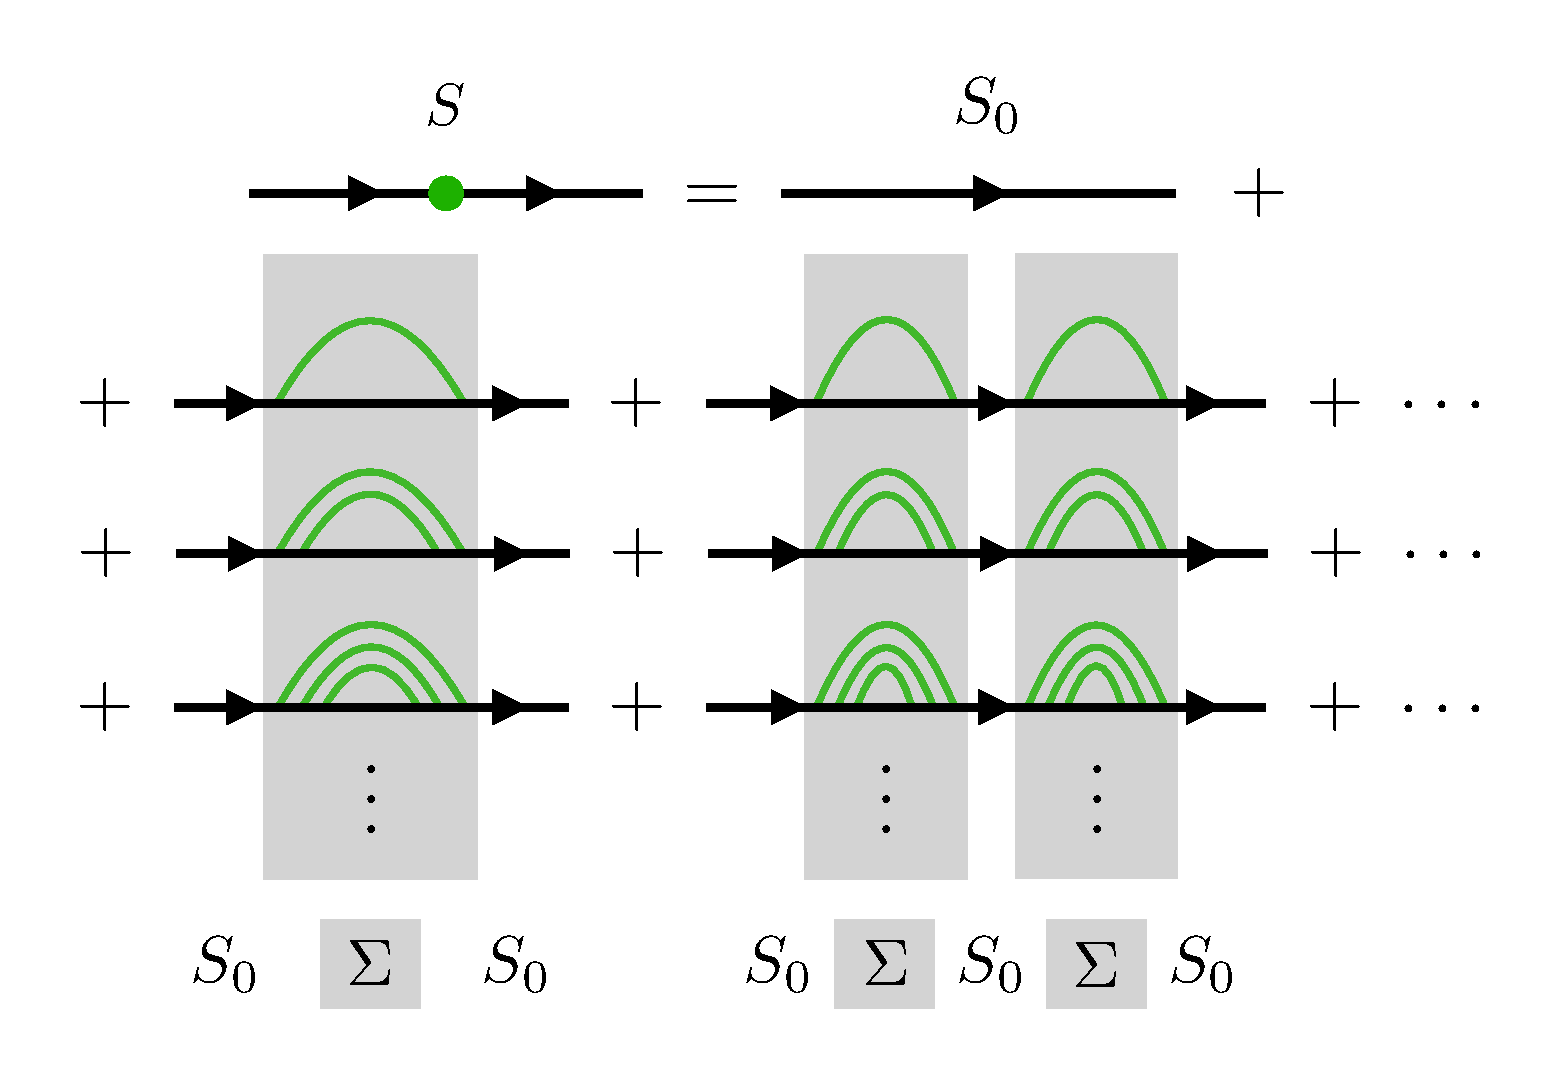
\includegraphics[width=.30\paperwidth]{Figures/chapter02/gap-equation}
		\end{center}

	\end{multicols}
  \vspace{-1em}

	We can find a relationship between these two by solving the \textbf{gap equation}:

	\begin{gather*}
		S^{-1} =
	    S_{0}^{-1} - 2iG_{\pi} \int \frac{\dd[2]{p}}{\qty(2\pi)^{2}}
	    N_\text{color} N_\text{flavor} \text{Tr}_\text{\tiny{D}}\qty[S] \\
	  M \simeq
	    m + 4iG_\pi N_\text{color} N_\text{flavor}
	    \int \frac{\dd[2]{p}}{(2\pi)^2} \frac{M}{p^2 - M^2}
	\end{gather*}

%% ----------------------------------------------------------------------------
\break
%% ----------------------------------------------------------------------------

	% To solve this last expression we first perform a \textbf{Wick rotation} $p_0 \ra i p_2 \qRa (p_0)^2 \ra - (p_2)^2$, followed by a transformation to \textbf{polar coordinates}:
  %
	% \begin{gather*}
	% 	M \simeq
	%     m + N_\text{color}  N_\text{flavor}
	%     \frac{G_\pi}{\pi} \int_{0}^{\infty} \frac{M}{p_E^2 + M^2} \dd{p_E^2}
	% \end{gather*}
  %
	% Finally, to make the integral converge, we introduce \textbf{proper time regularization}:
  %
	% \begin{gather*}
	%   \frac{1}{x^n} =
	%     \frac{1}{(n-1)!} \int_{0}^{\infty} \dd{\tau} \tau^{n-1} \exp[-\tau x] \ra
	%     \frac{1}{(n-1)!} \int_{1/\Lambda_{UV}^2}^{1/\Lambda_{IR}^2}
	%       \dd{\tau} \tau^{n-1} \exp[-\tau x] \\[5pt]
	%   M \simeq
	%     m + M N_\text{color} N_\text{flavor} \frac{G_\pi}{\pi}
	%     \int_{1/\Lambda_{UV}^2}^{1/\Lambda_{IR}^2} \frac{\dd{\tau}}{\tau}
	%     \exp[-\tau M^{2}]
	% \end{gather*}
  %
	% Where $\Lambda_{IR}$ and $\Lambda_{UV}$ are the \textbf{infrared and ultraviolet cutoffs} respectively.

%% ----------------------------------------------------------------------------
\break
%% ----------------------------------------------------------------------------

	\begin{center}
		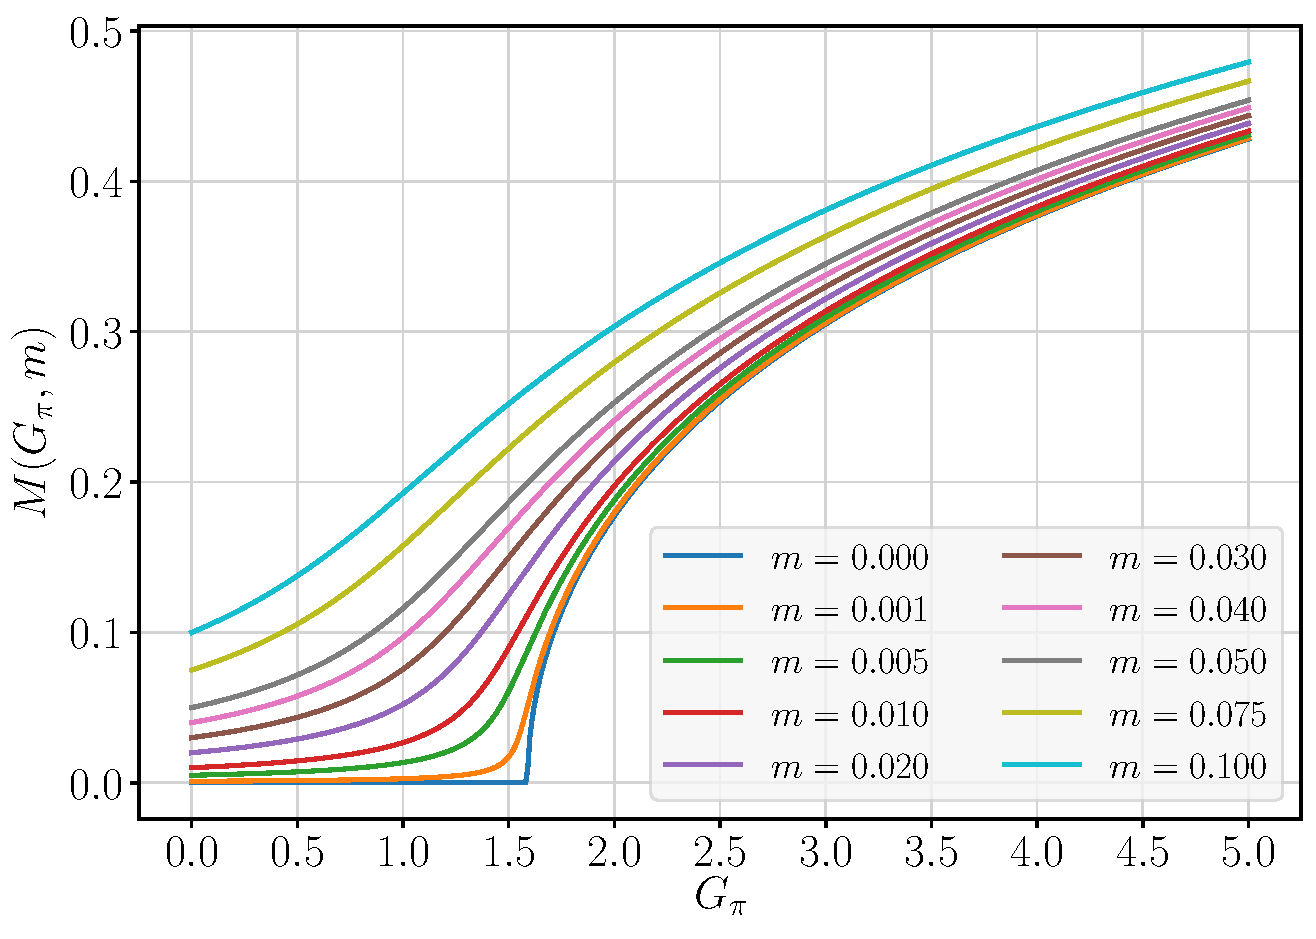
\includegraphics[width=.5\paperwidth]{Figures/chapter02/NJL-dressed-mass-curves}
	\end{center}

	\vspace{-1em}

	\begin{table}[!bp]
	  \centering
	  % \caption{Parameters used for solving the NJL model in $1+1$ dimensions.}
	  \label{tab:NJL1-analytical-solution-parameters}
	  \begin{tabular}{ c c c c c }
	    \hline
	    % \rule{0pt}{14pt}
	    $N_\text{Dirac}$ & $N_\text{color}$ & $N_\text{flavor}$ &
	    $\Lambda_{IR}$ & $\Lambda_{UV}$ \\
	    \hline
	    \hline
	    % \rule{0pt}{14pt}
	    $1+1 \ra 2$ & $1$ & $1$ & $0.240$ GeV & $0.645$ GeV \\
	    \hline
	  \end{tabular}
	\end{table}

\end{frame}


%% ----------------------------------------------------------------------------
%% LATTICE FORMULATION
%% ----------------------------------------------------------------------------

\subsection{Lattice formulation}

%% ----------------------------------------------------------------------------
%% ----------------------------------------------------------------------------

\begin{frame}[allowframebreaks]{Lattice formulation}

	We can define the Hamiltonian of the system as the integral over space of the Hamiltonian density:

	\begin{gather*}
		H = \int \mathcal{H}(x) \dd{x}
	    = \int \qty{
	      \bar{\psi}_{\alpha}(x)
	      \qty(\hat{m}_{\alpha\beta} - \delta_{\alpha\beta}i\gamma^{1}\partial_{1})
	      \psi_{\beta}(x) -
	      \frac{1}{2}G_{\pi}
	      \qty[\bar{\psi}_{\alpha}(x)\psi_{\alpha}(x)]^{2}} \dd{x}
	\end{gather*}

	For a basis where:

	\begin{gather*}
		\psi_{\alpha} = \mqty[\psi_{\alpha,+} \\ \psi_{\alpha,-}] \qc
	  \bar{\psi}_{\alpha} \defeq \psi^{\dagger}_{\alpha}\gamma^{0} \qc
		\gamma^{0} = \mqty[1 & 0\\ 0 & -1] \qc
	  \gamma^{1} = \mqty[0 & -1\\ 1 & 0]
	\end{gather*}

	Dropping the flavor indices to avoid clutter we can then write the kinetic term as:

	\begin{gather*}
	  \bar{\psi}\qty(-i\gamma^{1}\partial_{1})\psi =
			\frac{i}{2} \qty{
	      \qty[ \psi^{\dagger}_{+} \qty(\partial_{1}\psi_{-}) -
	      \qty(\partial_{1}\psi^{\dagger}_{+}) \psi_{-} ] +
	      \qty[ \psi^{\dagger}_{-} \qty(\partial_{1}\psi_{+}) -
	      \qty(\partial_{1}\psi^{\dagger}_{-}) \psi_{+} ]
	    }
	\end{gather*}

%% ----------------------------------------------------------------------------
\break
%% ----------------------------------------------------------------------------

	The two groups in brackets are essentially equivalent to one another by virtue of exchanging positive and negative energy components. This is the motivation behind \textbf{staggered fermion lattices}, which use two computational lattice sites for each theoretical value of $\psi$.

	\begin{figure}[!tbp]
		\centering
		\begin{minipage}[c]{.45\linewidth}
			\centering
			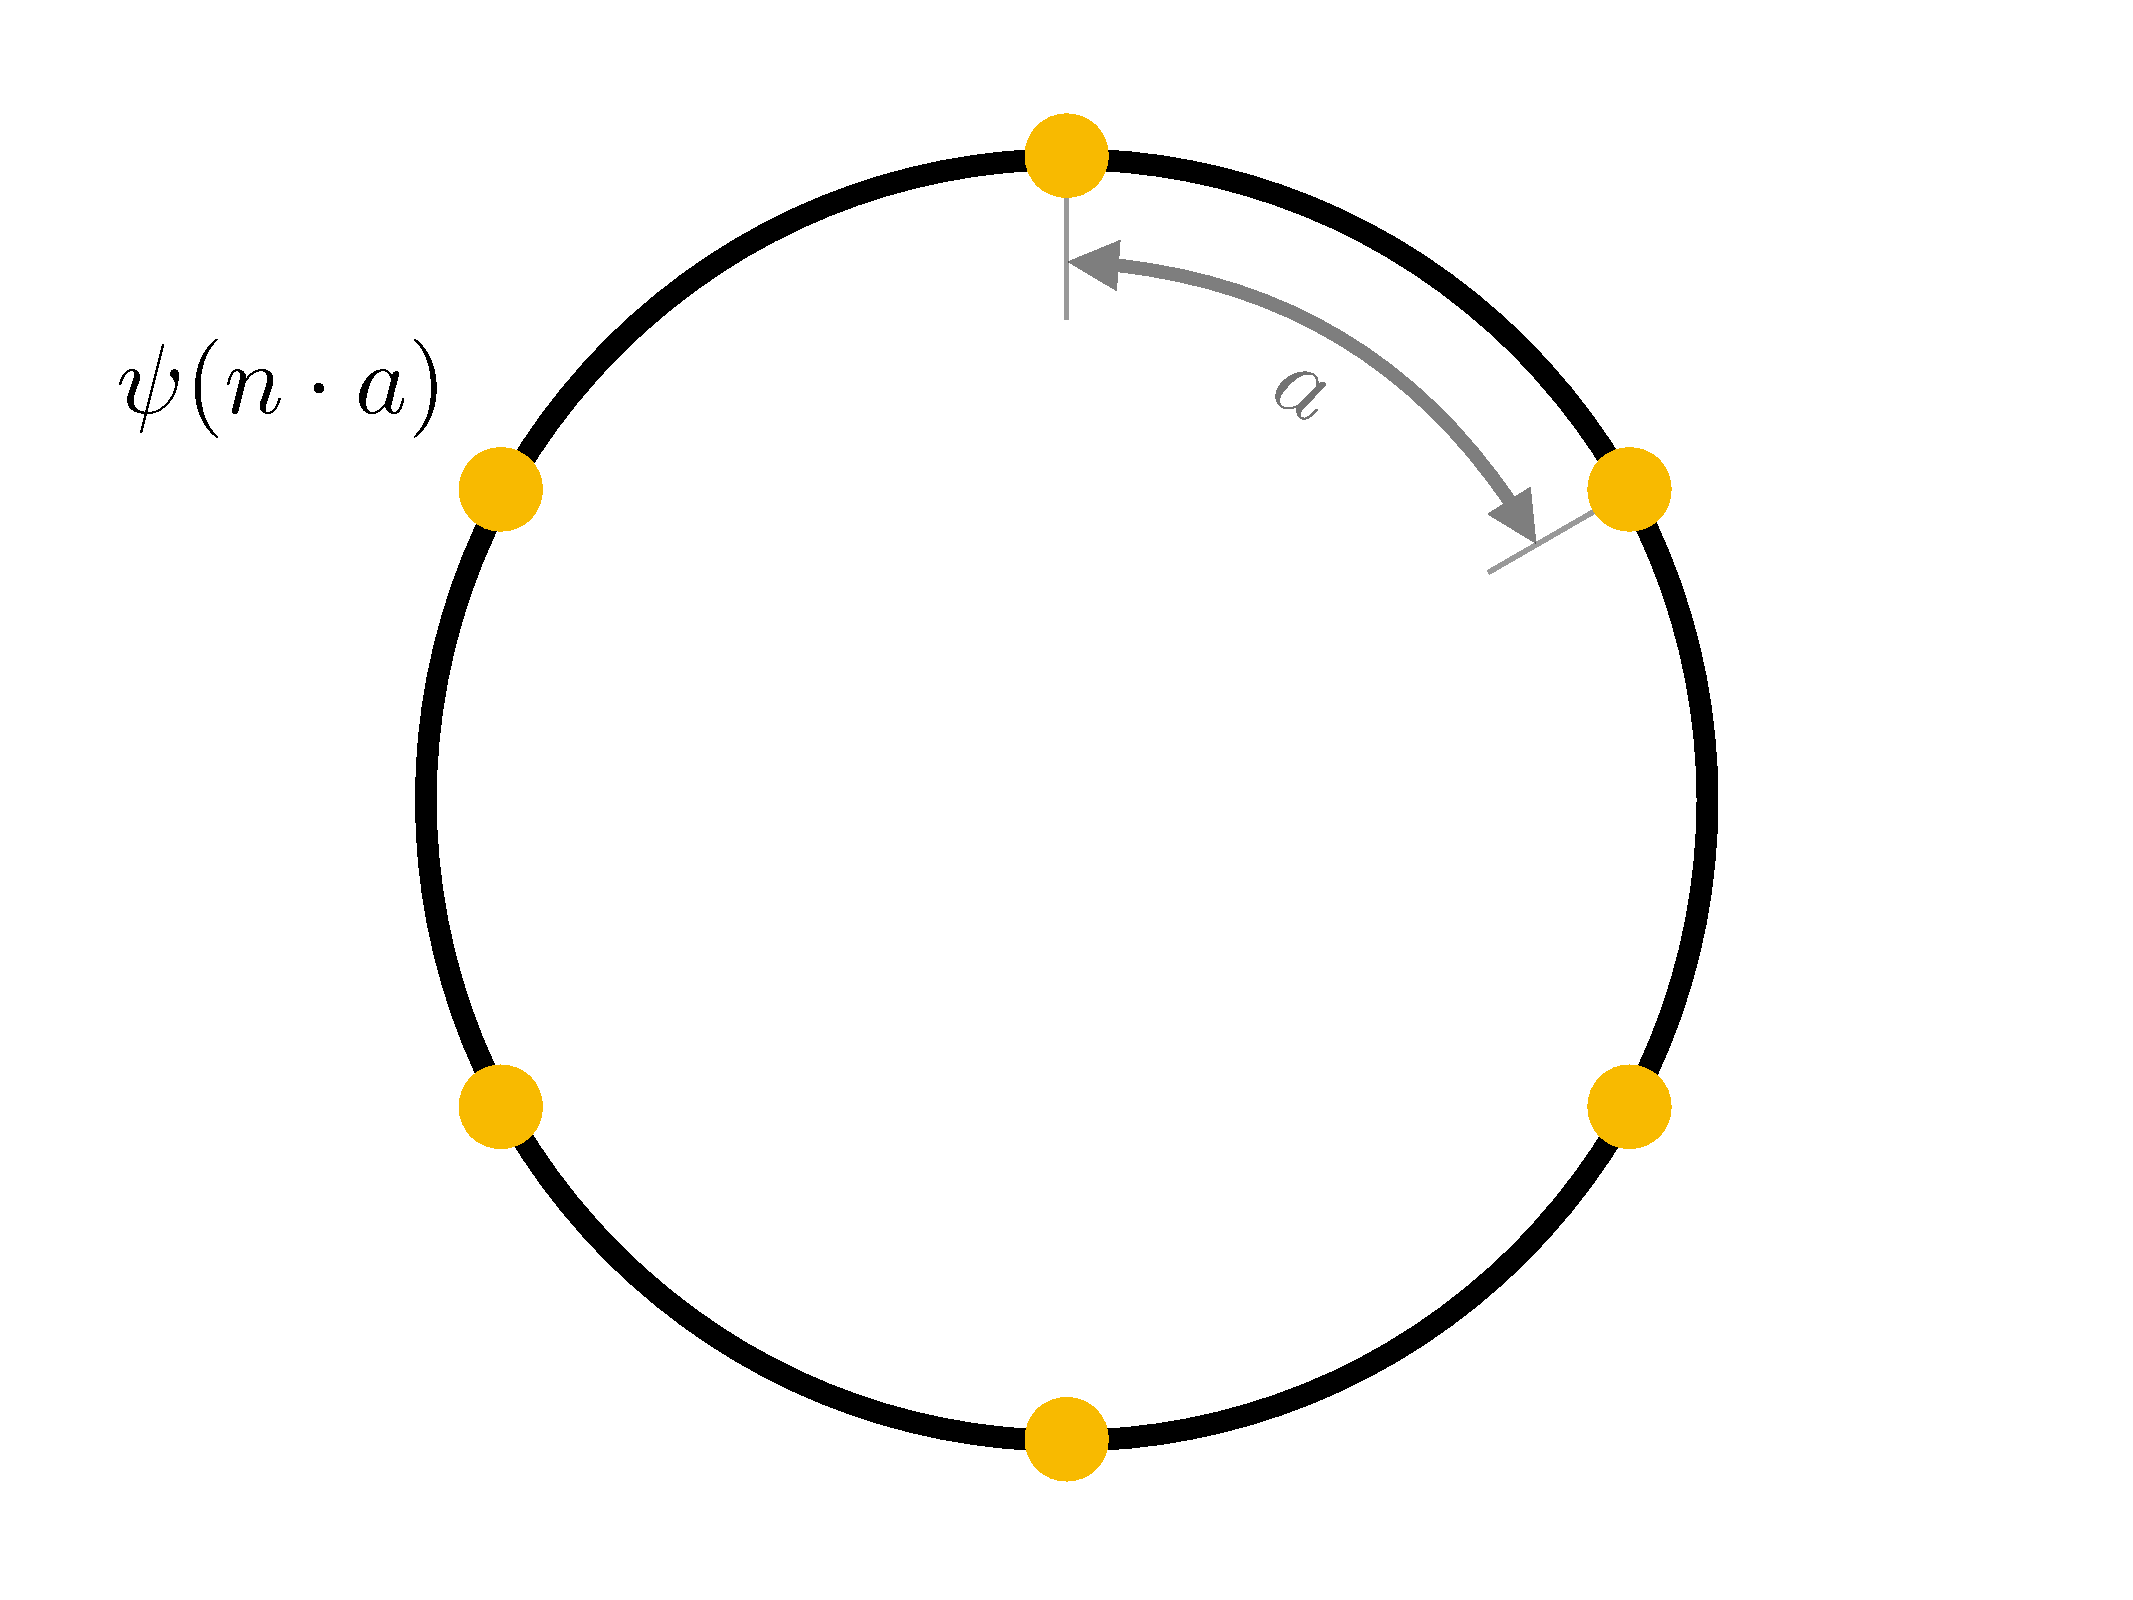
\includegraphics[width=\linewidth]{Figures/chapter02/physical-fermion-lattice}
		\end{minipage}
	  \hspace{.025\linewidth}
		\begin{minipage}[c]{.45\linewidth}
			\centering
			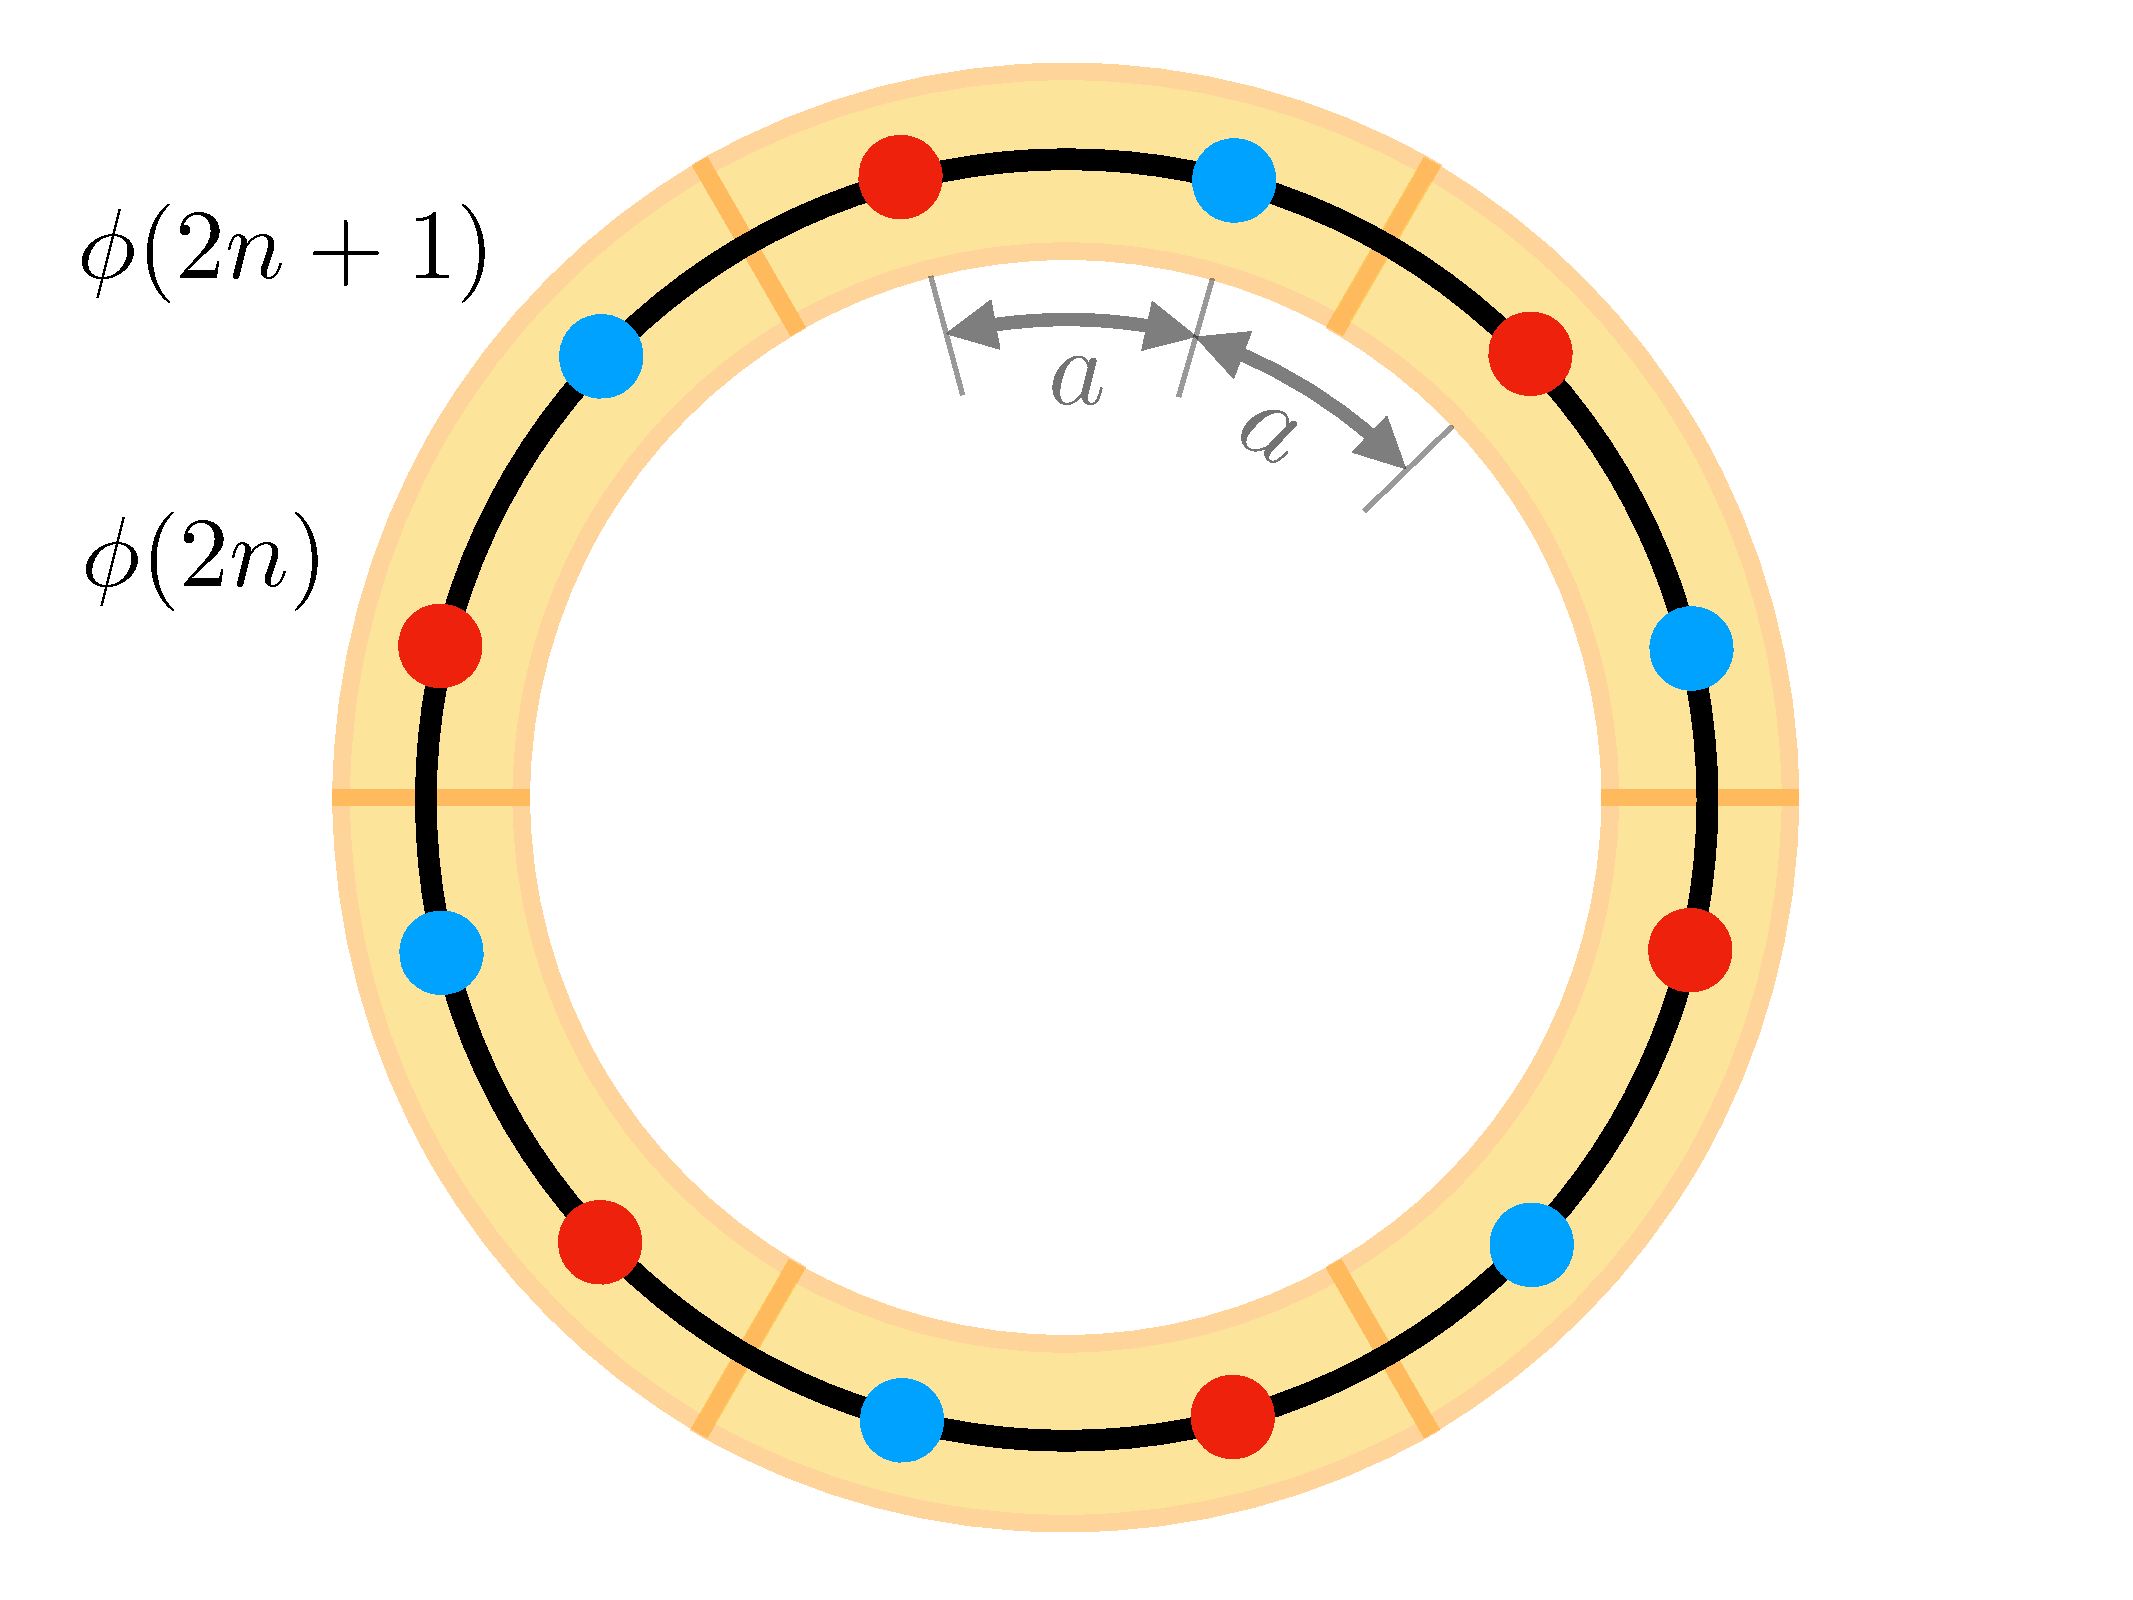
\includegraphics[width=\linewidth]{Figures/chapter02/computational-fermion-lattice}
		\end{minipage}
	\end{figure}

%% ----------------------------------------------------------------------------
\break
%% ----------------------------------------------------------------------------

	Sites in the staggered computational lattice are labeled using a parameter $n \in \mathds{Z}$ such that all evaluations of $\psi$ are made at integer multiples of the distance $a$:

	\begin{gather*}
	  \phi(n) \defeq \sqrt{a}
	    \begin{cases}
	      \psi_{+}\qty(\frac{n}{2}a) \qc &2 \mid n \\
	      \psi_{-}\qty(\frac{n-1}{2}a) \qc &2 \nmid n
	    \end{cases}
	\end{gather*}

	These newly defined operators obey the \textbf{canonical anti-commutation relations for fermions}:

	\begin{gather*} \label{eq:fermion-canonical-commutation-relations}
	  \acom{\phi^{\dagger}(p)}{\phi(q)} = \delta_{pq} \qc
	  \acom{\phi(p)}{\phi(q)} = 0
	\end{gather*}

	Finally, thanks to the periodic boundary conditions, we can write:

	\begin{gather*}
	  H_{N}^{(K)} =
	    \frac{i}{2a} \sum_{n=0}^{2N-1} \qty[
	    \phi^{\dagger}(n)\phi(n+1) - \phi^{\dagger}(n+1)\phi(n)]
	\end{gather*}

%% ----------------------------------------------------------------------------
\break
%% ----------------------------------------------------------------------------

	From this Hamiltonian, we can now recover the \textbf{masless Dirac equation} in the continuum limit; which serves as proof of correctness:

	\begin{gather*}
	  \dot{\phi}(n) =
      i\com{H_{N}^{(K)}}{\phi(n)} =
      \frac{\phi(n+1)-\phi(n-1)}{2a}
	\end{gather*}

	In terms of the original fields, this is:

	\begin{gather*}
	  \dot{\psi_{+}} = \frac{\Delta \psi_{-}}{\Delta x} \qc
	  \dot{\psi_{-}} = \frac{\Delta \psi_{+}}{\Delta x}
	\end{gather*}

	Lastly, taking the limit when $a \ra 0$:

	\begin{gather*}
	  \pderivative{t}\psi =
      \mqty[0 & 1 \\ 1 & 0] \pderivative{x}\psi \equiv
      \hat{\alpha}_1 \pderivative{x}\psi
	\end{gather*}

\end{frame}

%% ----------------------------------------------------------------------------
%% ----------------------------------------------------------------------------

\begin{frame}[allowframebreaks]{Multi-flavor lattice}

  To obtain the other components of the Hamiltonian from the expressions in the Hamiltonian density, which are written in terms of \textbf{Dirac bilinears}, we need to restore the flavor indices and deal with them in the computational lattice.

  \vspace{1em}
  Assuming that each flavor is independent, we could simply repeat the same procedure over different computational lattices and sum the results for all flavors. For instance, assuming that the \textbf{mass matrix is diagonal} (i.e. $\hat{m}_{\alpha\beta}=\text{diag}\qty[m_0,m_1,\ldots]$):

  \begin{align*}
  \int \bar{\psi}_{\alpha}\psi_{\alpha} \dd{x} \qra
    &\sum_{n=0}^{N-1}
      \qty[ \phi_{\alpha}^{\dagger}(2n)\phi_{\alpha}(2n) -
      \phi_{\alpha}^{\dagger}(2n+1)\phi_{\alpha}(2n+1) ] = \\
    &\sum_{n=0}^{2N-1} (-1)^{n}\phi_{\alpha}^{\dagger}(n)\phi_{\alpha}(n)
  \end{align*}

%% ----------------------------------------------------------------------------
\break
%% ----------------------------------------------------------------------------

  However the interaction will always introduce \textbf{cross-flavor terms} rendering this invalid:

  \begin{gather*}
  \int \qty(\sum_{\alpha}\bar{\psi}_{\alpha}\psi_{\alpha})^{2} \dd{x}
    \,=\,\,
    \int \qty[\sum_{\alpha} \qty(\bar{\psi}_{\alpha}\psi_{\alpha})^{2} +
    2\sum_{\alpha < \beta} \qty(\bar{\psi}_{\alpha}\psi_{\alpha})
    \qty(\bar{\psi}_{\beta}\psi_{\beta})] \dd{x}
  \end{gather*}

  To solve this, we will build a single computational lattice with all the components of the field associated to different flavors stitched together back-to-back. The resulting operators are:

  \begin{gather*}
  \phi_{\alpha}(n) \equiv \phi(n + 2N\alpha) \defeq \sqrt{a}
    \begin{cases}
      \psi_{\alpha,+}\qty(\frac{n}{2}a) \qc &2 \mid n \\
      \psi_{\alpha,-}\qty(\frac{n-1}{2}a) \qc &2 \nmid n
    \end{cases} \\[1em]
    \acom{\phi_{\alpha}^{\dagger}(p)}{\phi_{\beta}(q)} =
      \delta_{\alpha\beta}\delta_{pq} \qc
    \acom{\phi_{\alpha}(p)}{\phi_{\beta}(q)} = 0
  \end{gather*}

%% ----------------------------------------------------------------------------
\break
%% ----------------------------------------------------------------------------

  With \textbf{periodic boundary conditions} applied on each flavor separately (i.e. not crossing over to other flavors $\phi_\alpha(2N) = \phi_\alpha(0) \neq \phi_{\alpha+1}(0)$).

  \begin{figure}[!tbp]
    \centering
    \begin{minipage}[c]{.45\linewidth}
      \centering
      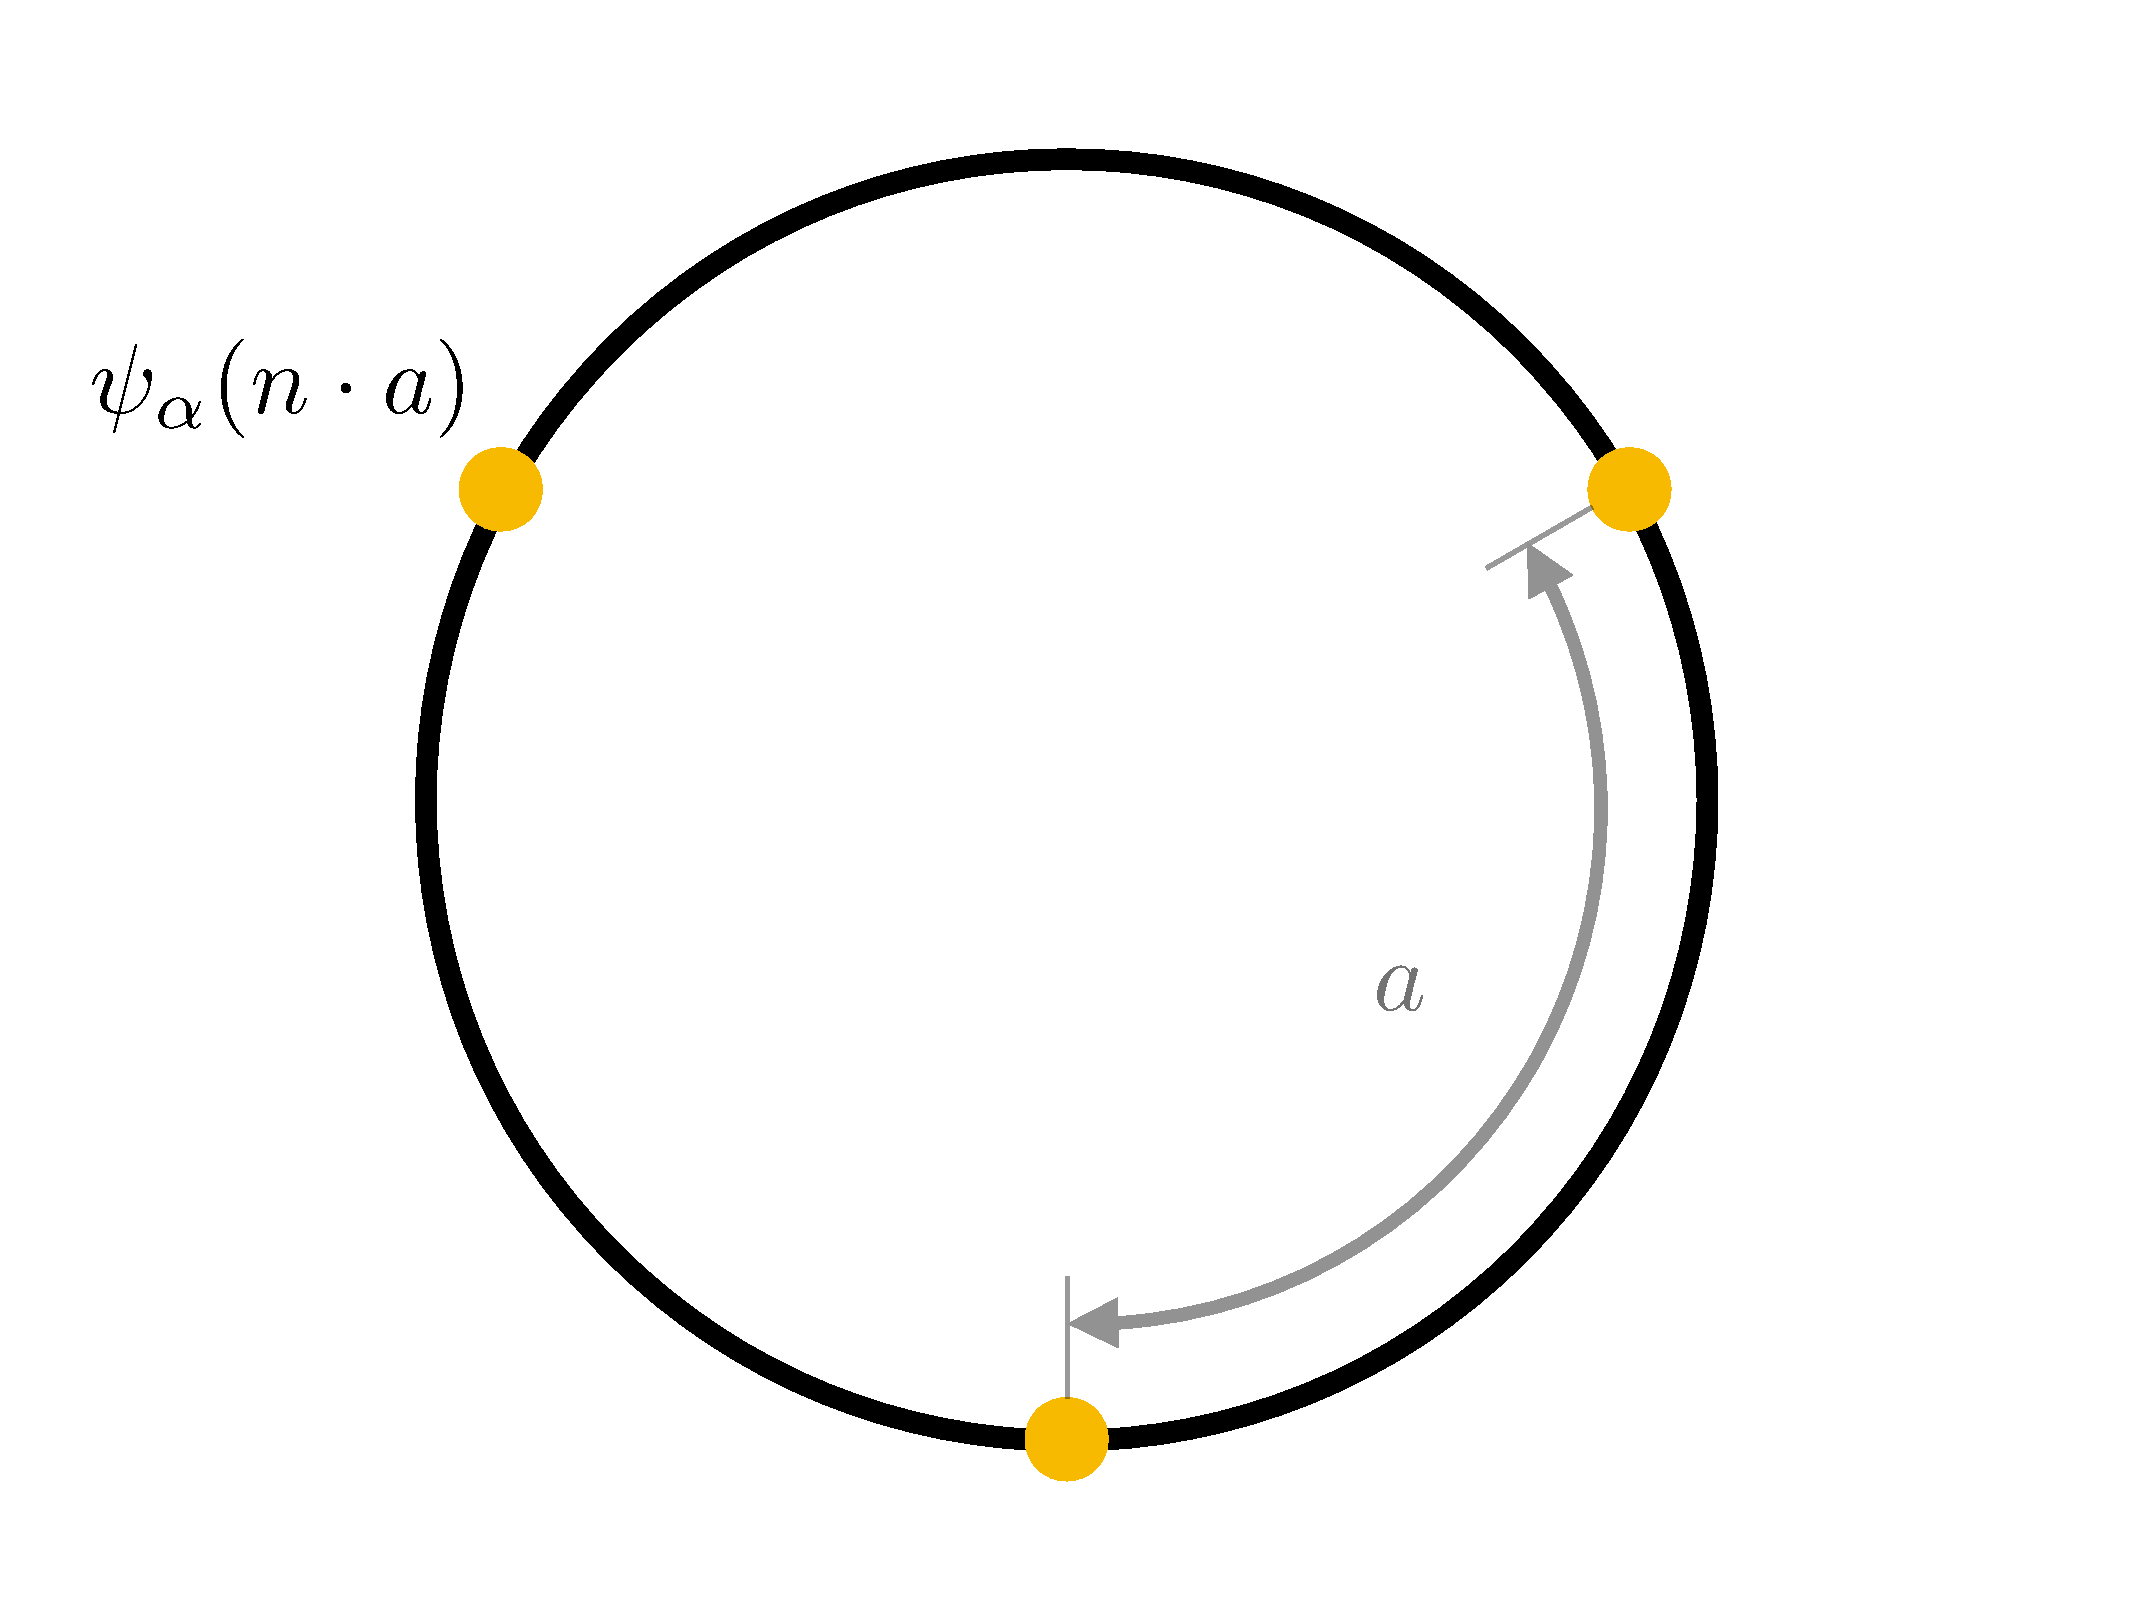
\includegraphics[width=\linewidth]{Figures/chapter02/physical-fermion-lattice-flavor}
    \end{minipage}
    \hspace{.025\linewidth}
    \begin{minipage}[c]{.45\linewidth}
      \centering
      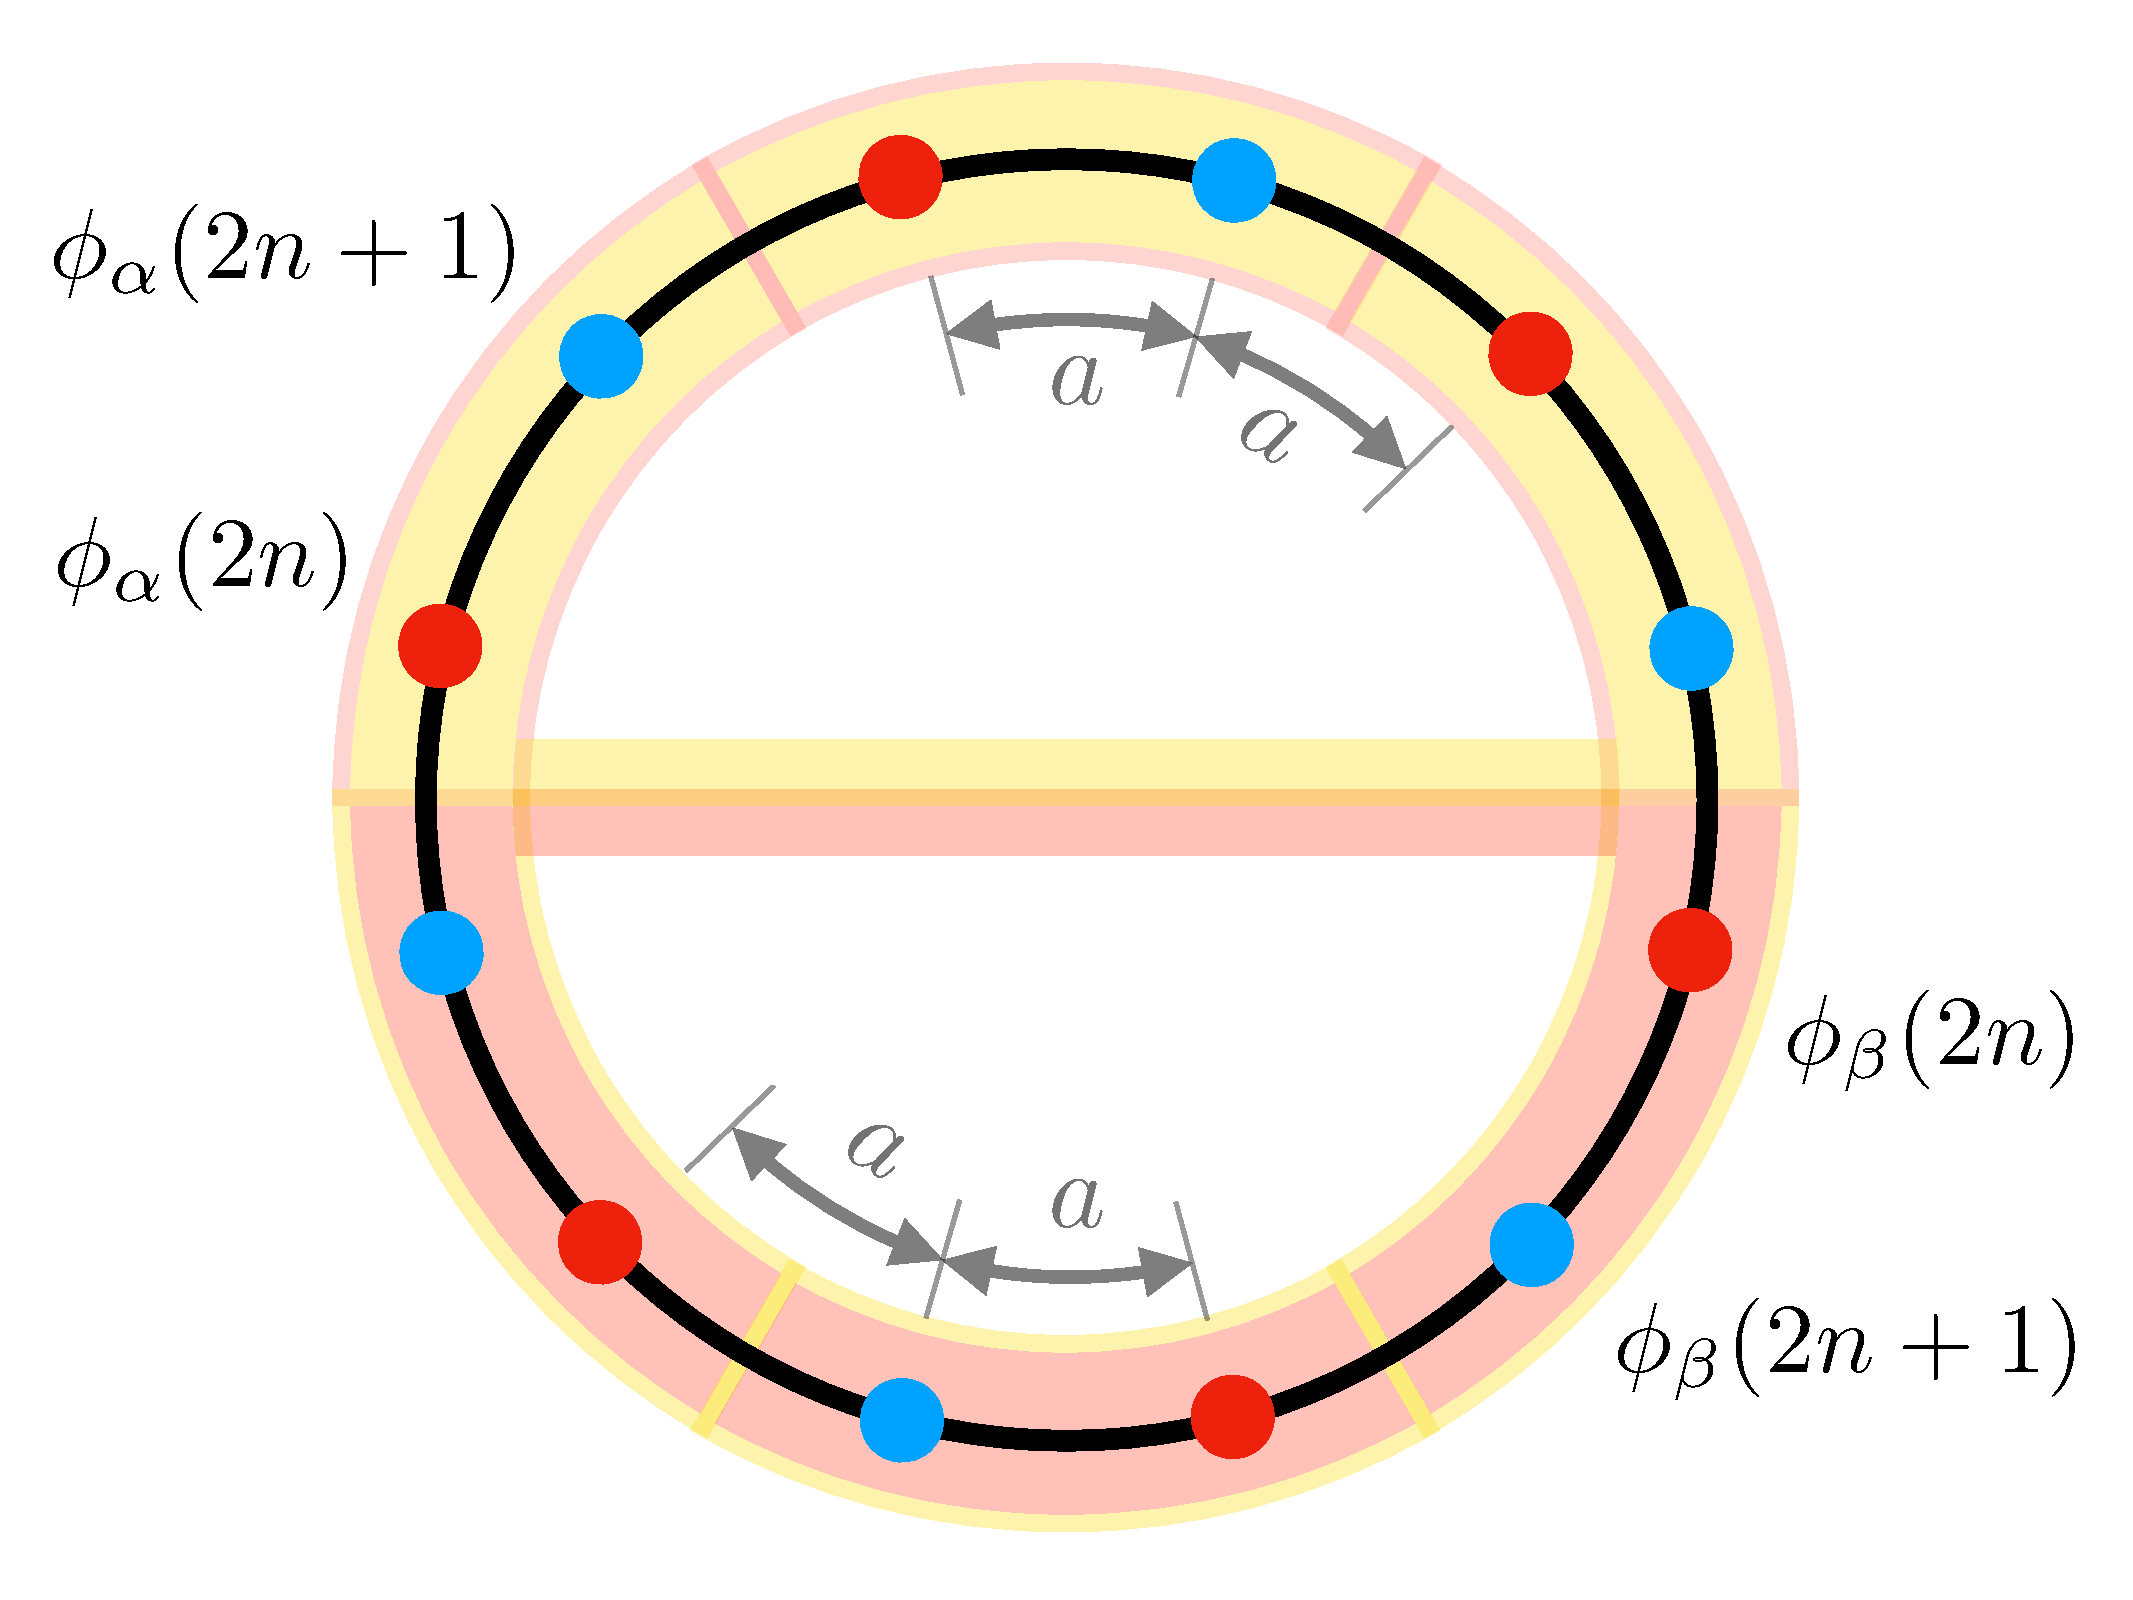
\includegraphics[width=\linewidth]{Figures/chapter02/computational-fermion-lattice-flavor}
    \end{minipage}
  \end{figure}

%% ----------------------------------------------------------------------------
\break
%% ----------------------------------------------------------------------------

  All in all, we obtain the following discretized NJL Hamiltonian for $1+1$ dimensions, any number of flavors $N_\text{flavor}$, $N$ physical lattice sites, and $2N\!\cdot\!N_\text{flavor}$ computational lattice sites:

  \begin{align*}
    H_{N} =&\, H_{N}^{(M)} + H_{N}^{(K)} + H_{N}^{(G)} \\
    H_{N}^{(M)} =&\,
      \sum_{\alpha} \sum_{n=0}^{2N-1}
      (-1)^{n} \, m_{\alpha} \phi_{\alpha}^{\dagger}(n)\phi_{\alpha}(n)  \\
    H_{N}^{(K)} =&\, \frac{i}{2a}
      \sum_{\alpha} \sum_{n=0}^{2N-1} \qty[
      \phi_{\alpha}^{\dagger}(n) \phi_{\alpha}(n+1) -
      \phi_{\alpha}^{\dagger}(n+1) \phi_{\alpha}(n)]  \\
    H_{N}^{(G)} =&\, - \frac{G_{\pi}}{2a} \sum_{n=0}^{N-1} \qty[
      \sum_{\alpha} \dbtilde{H}_{N}^{\alpha\alpha}(n) + 2
      \sum_{\alpha < \beta} \dbtilde{H}_{N}^{\alpha\beta}(n)]
  \end{align*}
  \begin{align*}
    \dbtilde{H}_{N}^{\alpha\beta}(n) \defeq&\,
      \qty[\phi_{\alpha}^{\dagger}(2n)\phi_{\alpha}(2n) -
      \phi_{\alpha}^{\dagger}(2n+1)\phi_{\alpha}(2n+1)] \times
      \qty[\phi_{\beta}^{\dagger}(2n)\phi_{\beta}(2n) -
      \phi_{\beta}^{\dagger}(2n+1)\phi_{\beta}(2n+1)]
  \end{align*}

\end{frame}

%%    _____  _____
%%   |  __ \|  __ \    AUTHOR: Pedro Rivero
%%   | |__) | |__) |   ---------------------------------
%%   |  ___/|  _  /    DATE: November 10, 2021
%%   | |    | | \ \    ---------------------------------
%%   |_|    |_|  \_\   https://github.com/pedrorrivero
%%

\section{Fermion-qubit mappings}

%% ----------------------------------------------------------------------------
%% ----------------------------------------------------------------------------

\begin{frame}{Fermion-qubit mappings}

	Generally speaking, quantum computers cannot work with any given operator directly. Therefore, in order to simulate this or any other Hamiltonian in a quantum processor, one needs to efficiently map its component operators onto ones suitable for operating in such machines. The most commonly used of these is the \textbf{Pauli set}.

  \begin{center}
    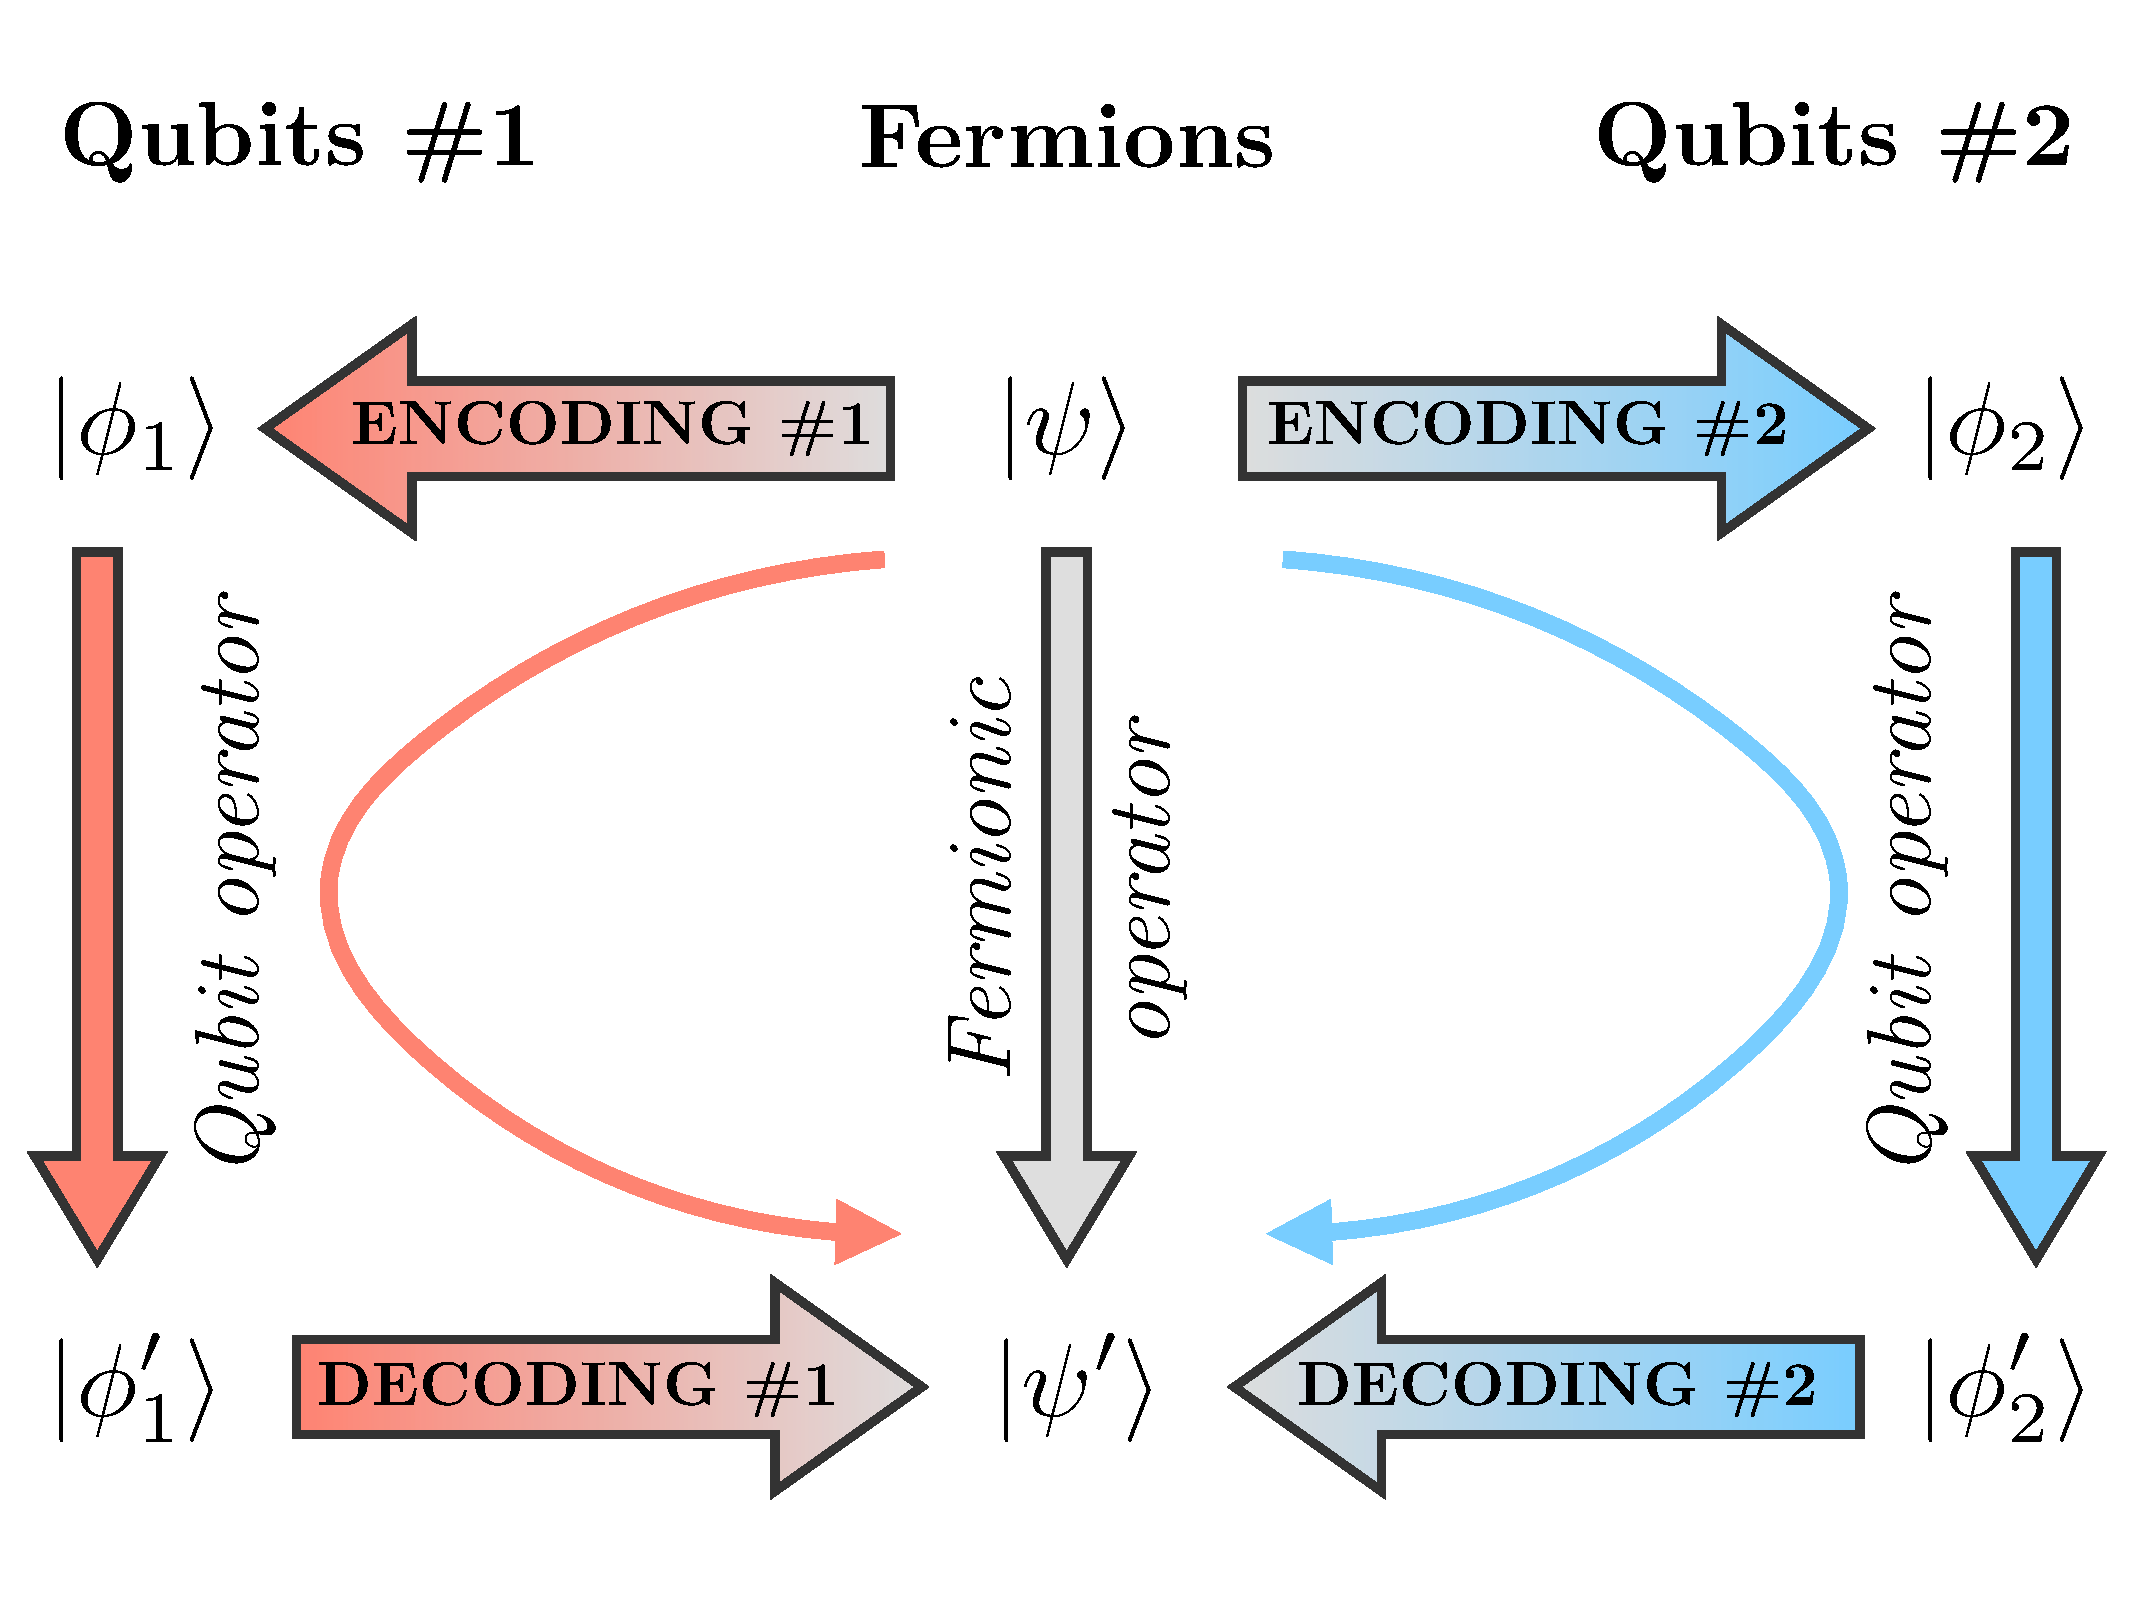
\includegraphics[width=.40\paperwidth]{Figures/chapter03/simulation-mapping}
  \end{center}

\end{frame}


%% ----------------------------------------------------------------------------
%% ----------------------------------------------------------------------------

\subsection{Jordan--Wigner mapping}

%% ----------------------------------------------------------------------------

\begin{frame}[allowframebreaks]{Jordan-Wigner mapping}

  The Pauli exclusion principle introduces a powerful liaison between fermions in the same quantum state. For this reason, even a non-interacting gas of fermions is still highly correlated. However, it turns out that in one spatial dimension spin-$\frac{1}{2}$ particles (i.e. qubits) behave much like fermions. Particularly, we choose:

  \begin{align*}
    \ket{\ua} \equiv \ket{0} &\qc
      \ket{\da} \equiv \ket{1} \\
    \ket{\da} \equiv \phi^{\dagger}\ket{0} &\qc
      \ket{\ua} \equiv \phi\ket{1} \\[5pt]
    \phi \ra \sigma^{+} &\qc \phi^{\dagger} \ra \sigma^{-}
  \end{align*}

  The mapping that the Jordan--Wigner transform introduces is designed on the \textbf{occupation number basis}, which associates spin ``down'' and ``up'' with occupied and unoccupied fermion states respectively. All this allows us to use these spins as a basic model for fermions:

	\begin{gather*}
	  \acom{\phi}{\phi^{\dagger}} = 1 \qra \acom{\sigma^{+}}{\sigma^{-}} = 1
	\end{gather*}

%% ----------------------------------------------------------------------------
\break
%% ----------------------------------------------------------------------------


	% To prove that this is valid, we can define the following equivalences by drawing inspiration from raising and lowering operators in angular momentum theory:
  %
	% \begin{align*}
	% 	\sigma^{1} &\equiv \phi^{\dagger} + \phi \\
	% 	\sigma^{2} &\equiv i\qty(\phi^{\dagger} - \phi) \\
	% 	\sigma^{3} &\equiv 1 - 2\phi^{\dagger}\phi
	% \end{align*}
  %
	% Making use of the properties of fermion creation and annihilation operators, comprised within their canonical commutation relations, these can be shown to behave algebraically like \textbf{Pauli matrices}:
  %
	% \begin{align*}
	%   \com{\sigma^{p}}{\sigma^{q}} &= 2i\epsilon_{pqr}\sigma^{r} \\
	%   \acom{\sigma^{p}}{\sigma^{q}} &= 2\delta_{pq}
	% \end{align*}

%% ----------------------------------------------------------------------------
% \break
%% ----------------------------------------------------------------------------

	% We can recover the usual spin raising and lowering hermitian conjugate operators:
  %
	% \begin{gather*}
	%   \sigma^{\pm} \defeq \frac{1}{2}\qty(\sigma^{1} \pm i\sigma^{2})
	% \end{gather*}
  %
	% All this allows us to use these spins as a basic model for fermions:
  %
	% \begin{gather*}
	%   \acom{\phi}{\phi^{\dagger}} = 1 \qra \acom{\sigma^{+}}{\sigma^{-}} = 1
	% \end{gather*}
  %
  % \break

	Unfortunately, this only works for single-fermion representations; since independent spins commute, while independent fermions anticommute.

	\begin{gather*}
	  \com{\sigma^{+}(p)}{\sigma^{-}(q)} = \delta_{pq} \qc
	    \acom{\sigma^{+}(p)}{\sigma^{-}(q)} \neq \delta_{pq} \\
	  \com{\phi(p)}{\phi^{\dagger}(q)} \neq \delta_{pq} \qc
	    \acom{\phi(p)}{\phi^{\dagger}(q)} = \delta_{pq}
	\end{gather*}

%% ----------------------------------------------------------------------------
% \break
%% ----------------------------------------------------------------------------

	A way to fix this issue is by defining $N(l)=\phi^{\dagger}(l)\phi(l)$ as the hermitian number operator for state $l$, and attaching a so called unitary \textbf{string operator} $S(n)$ to the fermion operators:

	\begin{gather*}
		\begin{split}
			S(n)\phi(n) \ra \sigma^{+}(n) \qc
			\phi^{\dagger}(n)S^{\dagger}(n) \ra \sigma^{-}(n)
		\end{split} \\
		S(n) = \exp[ -i\pi {\textstyle\sum_{l<n}} \qty[N(l)+s(l)] ]
	\end{gather*}

	The $s(l)$ terms in the string operator are scalars associated to \textbf{gauge transformations}.% and do not add much to the transform.% With this new mapping, Pauli matrices get redefined to:

	% \begin{align*}
	% 	\sigma^{1}(n) &\equiv
	% 		\phi^{\dagger}(n)S^{\dagger}(n) + S(n)\phi(n) \\
	% 	\sigma^{2}(n) &\equiv
	% 		i\qty[\phi^{\dagger}(n)S^{\dagger}(n) - S(n)\phi(n)] \\
	% 	\sigma^{3}(n) &\equiv
	% 		1 - 2\phi^{\dagger}(n)\phi(n)
	% \end{align*}

%% ----------------------------------------------------------------------------
\break
%% ----------------------------------------------------------------------------

	We now retrieve the correct statistics. Of course, we would like to express the string operator in terms of the Pauli set so that we can move it to the other side of the transformation. Fortunately, we can do so by expanding the number operators:

	\begin{gather*}
	  \exp[\pm i\pi \sum_{l<n} N(l)] =
		  \prod_{l<n}\exp[\pm i\pi \phi^{\dagger}(l)\phi(l)] =
		  \prod_{l<n}\qty[1-2\phi^{\dagger}(l)\phi(l)] =
		  \prod_{l<n}\sigma^3(l) \\
		S(n) = \prod_{l<n} e^{-i\pi s(l)} \sigma^3(l)
	\end{gather*}

	Finally, our \textbf{choice of gauge} will be such that $s(l) = s \in (-1,1]$ $\forall l$ and the string operator is hermitian for all values of $n$. All in all, this can be achieved by making $s=0$, which gives:

	\begin{gather*}
		\phi(n) \ra \qty[\prod_{l<n} \sigma^3(l)]\sigma^{+}(n) \qc
		\phi^{\dagger}(n) \ra \qty[\prod_{l<n} \sigma^3(l)]\sigma^{-}(n)
	\end{gather*}

%% ----------------------------------------------------------------------------
% \break
%% ----------------------------------------------------------------------------

  % Lastly, we need to bring back flavor indices. The form of the transform will in fact be the same but, for clarity, we would like to write them down them explicitly. This will prove to be useful when dealing with the periodic boundary conditions. For this, all we need recalling is that the flavor sub-lattices had been stitched back-to-back in the final computational lattice:
  %
  % \begin{gather*}
  %   \phi_\alpha(n) \ra S_\alpha(n) \sigma_\alpha^{+}(n) =
  %     \qty[\prod_{\beta=0}^{\alpha-1} \tilde{\sigma}_\beta^{3}(2N)]
  %     \tilde{\sigma}_\alpha^{3}(n) \sigma_\alpha^{+}(n) \\
  %   \phi_\alpha^\dagger(n) \ra S_\alpha^\dagger(n) \sigma_\alpha^{-}(n) =
  %     \qty[\prod_{\beta=0}^{\alpha-1} \tilde{\sigma}_\beta^{3}(2N)]
  %     \tilde{\sigma}_\alpha^{3}(n) \sigma_\alpha^{-}(n)
  % \end{gather*}
  % \begin{gather*}
  %   S_\alpha(n) \defeq S(n + 2N\alpha) \qqc
  %   \tilde{\sigma}_\alpha^{3}(n) \defeq \prod_{l<n} \sigma_\alpha^{3}(l)
  % \end{gather*}

\end{frame}

%% ----------------------------------------------------------------------------
%% ----------------------------------------------------------------------------

\subsection{Refactoring NJL}

%% ----------------------------------------------------------------------------

\begin{frame}[allowframebreaks]{Refactoring the NJL Hamiltonian}

  % Now that we have a way of converting from fermion to spin operators, let's apply it to the NJL Hamiltonian. To do so, we will make use of the Jordan--Wigner transform, and it is convenient to note some previous mappings first:
  %
  % \begin{align*}\begin{split}
  %   \phi_\alpha^{\dagger}(n)\phi_\alpha(n) &\qra
  %     \frac{1}{2} \qty[1 - \sigma_\alpha^{3}(n)] \\
  %   \phi_\alpha^{\dagger}(n)\phi_\alpha(n) -
  %     \phi_\alpha^{\dagger}(n+1)\phi_\alpha(n+1) &\qra
  %     \frac{1}{2}\qty[\sigma_\alpha^{3}(n+1) - \sigma_\alpha^{3}(n)] \\
  %   \phi_\alpha^{\dagger}(n)\phi_\alpha(n+1) &\qra
  %     \sigma_\alpha^{-}(n)\sigma_\alpha^{+}(n+1) \\
  %   \phi_\alpha^{\dagger}(n+1)\phi_\alpha(n) &\qra
  %     \sigma_\alpha^{-}(n+1)\sigma_\alpha^{+}(n) \\
  %   \phi_\alpha^{\dagger}(n)\phi_\alpha(n+1) -
  %     \phi_\alpha^{\dagger}(n+1)\phi_\alpha(n) &\qra
  %     \frac{1}{2i} \qty[
  %       \sigma_\alpha^{1}(n+1) \sigma_\alpha^{2}(n) -
  %       \sigma_\alpha^{2}(n+1) \sigma_\alpha^{1}(n)
  %     ]
  % \end{split}\end{align*}

%% ----------------------------------------------------------------------------
% \break
%% ----------------------------------------------------------------------------

	Hence, bringing back flavor indices, the different parts of the Hamiltonian are:

  \begin{align*}
    H_{N}^{(M)} \qra&
      \frac{m}{2} \sum_\alpha \sum_{n=0}^{2N-1}
      (-1)^{n+1}\sigma_\alpha^{3}(n) \\
    H_{N}^{(K)} \qra&
      \frac{1}{4a} \sum_\alpha \sum_{n=0}^{2N-2}
      \qty[
        \sigma_\alpha^{1}(n+1) \sigma_\alpha^{2}(n) -
        \sigma_\alpha^{2}(n+1) \sigma_\alpha^{1}(n)
      ] + \nonumber\\&
      \frac{1}{4a} \sum_\alpha \!
      \qty[\prod_{l=1}^{2N-2} \!\! \sigma_\alpha^3(l)] \!
      \qty[
        \sigma_\alpha^{1}(0) \sigma_\alpha^{2}(2N \!-\! 1) -
        \sigma_\alpha^{2}(0) \sigma_\alpha^{1}(2N \!-\! 1)
      ] \\
    H_{N}^{(G)} \quad=\quad& - \frac{G_{\pi}}{2a} \sum_{n=0}^{N-1} \qty[
      \sum_{\alpha} \dbtilde{H}_{N}^{\alpha\alpha}(n) + 2
      \sum_{\alpha < \beta} \dbtilde{H}_{N}^{\alpha\beta}(n)] %\\
    % \dbtilde{H}_{N}^{\alpha\beta}(n) \qra&
    %   \frac{1}{4} \sum_{{j=0}\atop{k=0}}^{1}
    %   (-1)^{j+k} \, \sigma_\alpha^{3}(2n+j) \, \sigma_\beta^{3}(2n+k) \qc
  \end{align*}

%% ----------------------------------------------------------------------------
\break
%% ----------------------------------------------------------------------------

  \begin{gather*}
    \dbtilde{H}_{N}^{\alpha\beta}(n) \qra
      \frac{1}{4} \sum_{{j=0}\atop{k=0}}^{1}
      (-1)^{j+k} \, \sigma_\alpha^{3}(2n+j) \, \sigma_\beta^{3}(2n+k) \qc
  \end{gather*}

  It is important to notice that the periodic boundary conditions only enter through the kinetic term, and are responsible for the only non-local contribution. Finally, it is useful to note that:

  \begin{gather*}
    \dbtilde{H}_{N}^{\alpha\alpha}(n) \qra
      \frac{1}{2} \qty[1 - \sigma_\alpha^{3}(2n+1) \, \sigma_\alpha^{3}(2n)] \qc
  \end{gather*}

  which shows an extensive \textbf{adiabatic modification} term of the form $\frac{G_\pi}{4} N_\text{flavor} \times \frac{N}{a}$ in the interaction Hamiltonian (i.e. coming from the unit matrix). This term gathers the two usual singularities from Quantum Field Theory: one with the size of the system as it gets larger (i.e. $\sim N$), and the other on the continuum limit (i.e. $\sim 1/a$). We drop it as a vacuum contribution.

\end{frame}

%%    _____  _____
%%   |  __ \|  __ \    AUTHOR: Pedro Rivero
%%   | |__) | |__) |   ---------------------------------
%%   |  ___/|  _  /    DATE: November 10, 2021
%%   | |    | | \ \    ---------------------------------
%%   |_|    |_|  \_\   https://github.com/pedrorrivero
%%

\section{State preparation}

%% ----------------------------------------------------------------------------
%% ----------------------------------------------------------------------------

\begin{frame}[allowframebreaks]{Space parametrization and state preparation}

  We need to find ways of exploring different quantum states --- a process known as \textbf{state preparation}. In principle, with a good mapping, this can be achieved by parametrizing the Hilbert/Fock space of states representing the system, and finding a way to prepare the corresponding quantum state in the processor. Nonetheless:

  \begin{itemize}
    \item<2-> We are significantly constrained by the type of operations allowed on the qubits.
    \item<3-> The dimension of the space at hand grows exponentially with the number of qubits used in the representation of the system.
    \item<3-> We will be interested in finding a smaller subspace containing the solution to our problem.
    \item<4-> Randomized, and other naive general approaches suffer from problems such as \textbf{barren-plateaus} and \textbf{suboptimal local minima}.
    \item<4-> Useful to have some physical intuition to constrain the amount of states that we explore; which leads to problem specific ansatezs.
    \item Typically divided in: (1) prepare initial state, and (2) perform a parametrized evolution.
  \end{itemize}

\end{frame}
%% ----------------------------------------------------------------------------
%% ----------------------------------------------------------------------------

\subsection{HVA}

%% ----------------------------------------------------------------------------
%% ----------------------------------------------------------------------------

\begin{frame}[allowframebreaks]{Hamiltonian Variational Ansatz (HVA)}

  There is a family of circuits known as the Hamiltonian Variational Ansatz (HVA) --- also referred to as the QAOA ansatz --- which are based on \textbf{adiabatic state preparation}.

  \begin{theorem}[Simplified adiabatic theorem]
    Under a slowly changing Hamiltonian $H(t)$ with instantaneous eigenstates $\ket{n(t)}$ and corresponding energies $E_{n}(t)$, a quantum system initialized in a particular eigenstate $\ket{m(0)}$, will remain in the corresponding eigenstate $\ket{m(t)}$ during the evolution.
    % Under a slowly changing Hamiltonian $H(t)$ with instantaneous eigenstates $\ket{n(t)}$ and corresponding energies $E_{n}(t)$, a quantum system evolves from the initial state ${|\psi (0)\rangle =\sum _{n}c_{n}(0)|n(0)\rangle }$ to the final state ${|\psi (t)\rangle =\sum _{n}c_{n}(t)|n(t)\rangle}$ where the coefficients undergo the change of phase ${c_{n}(t)=c_{n}(0)e^{i\theta _{n}(t)}e^{i\gamma _{n}(t)}}$.
    % In particular, ${|c_{n}(t)|^{2}=|c_{n}(0)|^{2}}$, so if the system begins in an eigenstate of ${H(0)}$, it remains in an eigenstate of $H(t)$ during the evolution with a change of phase only.
  \end{theorem}

  Therefore, if we prepare an eigenstate $\ket{\varepsilon_0(0)}$ of one of the sub-Hamiltonians $H_0$, and slowly activate the others through activation parameters $\lambda_j(t)$, where $\lambda_j(0) = 0$, $\lambda_j(t \ra \infty) = 1$, and $\dot{\lambda}_j(t) \ll 1$; we will end up with the corresponding eigenstate $\ket{\varepsilon}$ for the entire Hamiltonian:

  \begin{gather*}
    \ket{\varepsilon} = \lim_{t \ra \infty}
      \exp[-i t \qty(H_0 + \sum_{j=1} \lambda_j(t) H_j)]
      \ket{\varepsilon_0(0)}
  \end{gather*}

%% ----------------------------------------------------------------------------
\break
%% ----------------------------------------------------------------------------

  Particularly, making use of the non-commuting terms in the Hamiltonian and a simple \textbf{Trotter decomposition} we can simulate this process digitally:

  \begin{gather*}
    H =
      \sum_{j}{H_j} \qc \com{H_j}{H_{k}} \neq 0 \quad\forall\, j \neq k \\[1em]
    \ket{\psi} = \exp[-i t H(t)] \ket{\psi_0} \approx
      \qty[ \prod_{k}^{p} \exp[-i \Delta t_k H(t_k)] ] \ket{\psi_0} =
      \qty[ \prod_{k}^{p} \exp[-i \Delta t_k \sum_j \lambda_j(t_k) H_j] ]
      \ket{\psi_0} \\
    \ket{\psi} \approx \prod_{k}^{p}
      \qty[\prod_{j} \exp[-i \Delta t_k \lambda_j(t_k) H_j]] \ket{\psi_0}
  \end{gather*}

%% ----------------------------------------------------------------------------
\break
%% ----------------------------------------------------------------------------

  Which, by noticing that we can control both the time steps as well as the activation parameters at will, leads to the final form of the parameterization ansatz:

  \begin{gather*}
    \ket{\psi\qty(\theta)} \defeq \prod_{k}^{p}
      \qty[\prod_{j} \exp(-i \theta_{jk} H_j)] \ket{\psi_0}
  \end{gather*}

  where $p$ is a variable parameter that stands for the depth of the ansatz. This technique is thought to possess \textbf{favorable properties} for solving optimization problems. Specifically, these circuits have been shown to display mild or entirely absent barren plateaus, as well as almost trap-free target landscapes.

  \medskip

  We also infer that the \textbf{initial state} $\ket{\psi_0}$ should be an eigenstate of one of the sub-Hamiltonians --- according to the output eigenstate that we want to obtain. Notice that this ansatz is indeed problem specific, since it depends on the Hamiltonian of the system of interest, and physically sound as well. Finally, most of the times it is enough to have $\com{H_j}{H_{j+1}} \neq 0 \ \forall j$.

\end{frame}

%%    _____  _____
%%   |  __ \|  __ \    AUTHOR: Pedro Rivero
%%   | |__) | |__) |   ---------------------------------
%%   |  ___/|  _  /    DATE: November 10, 2021
%%   | |    | | \ \    ---------------------------------
%%   |_|    |_|  \_\   https://github.com/pedrorrivero
%%

\section{Variational algorithms}

%% ----------------------------------------------------------------------------
%% ----------------------------------------------------------------------------

\begin{frame}[allowframebreaks]{Variational algorithms}

  One of the most promising near-term applications of quantum computers is the simulation of quantum mechanics. This is because:

  \begin{itemize}
    \item<2-> Quantum phenomena are exponentially hard to recreate by classical means, whilst thought to be efficiently reproducible using quantum resources: \textbf{quantum advantage}.
    \item<3-> This task is believed to be achievable in the foreseeable future thanks to \textbf{hybrid quantum-classical variational algorithms}.
    \item<4-> Promising applicability, especially for relatively low amounts of quantum resources: \textbf{Noisy Intermediate-Scale Quantum} era (NISQ).
  \end{itemize}

%% ----------------------------------------------------------------------------
\break
%% ----------------------------------------------------------------------------

  \begin{theorem}[Variational theorem]
    If the state $\ket{\psi}$ of a quantum system depends on some array of $n$ parameters $\qty{\theta^{n}}$, the optimal choice to approximate the ground state of said system (i.e. the eigenstate of its Hamiltonian $\hat{H}$ with minimum eigenvalue $\lambda_{\textnormal{min}}$) is the one which minimizes its Hamiltonian's expectation value $\ev*{\hat{H}}$. Assuming $\braket*{\psi}=1$:

    \begin{gather*}
      \ev{H}\!\qty(\theta^{n}) \equiv
        \ev{H}{\psi\qty(\theta^{n})} \geq
        \lambda_{\textnormal{min}} \, .
    \end{gather*}
  \end{theorem}

  Evaluating the expectation value of the different components making up our Hamiltonian is done through a process known as \textbf{operator averaging}:

  \begin{gather*}
    H_{N} = \sum_{j=1}^{\text{Poly}(N)} w_{j} P_{N}^{(j)} \qRa
    \ev{H_{N}} = \sum_{j=1}^{\text{Poly}(N)} w_{j} \ev{P_{N}^{(j)}}
  \end{gather*}

\end{frame}

%% ----------------------------------------------------------------------------
%% ----------------------------------------------------------------------------

\subsection{VQE and SSVQE}

%% ----------------------------------------------------------------------------
%% ----------------------------------------------------------------------------

\begin{frame}{Variational Quantum Eigensolver (VQE)}

	\begin{center}
		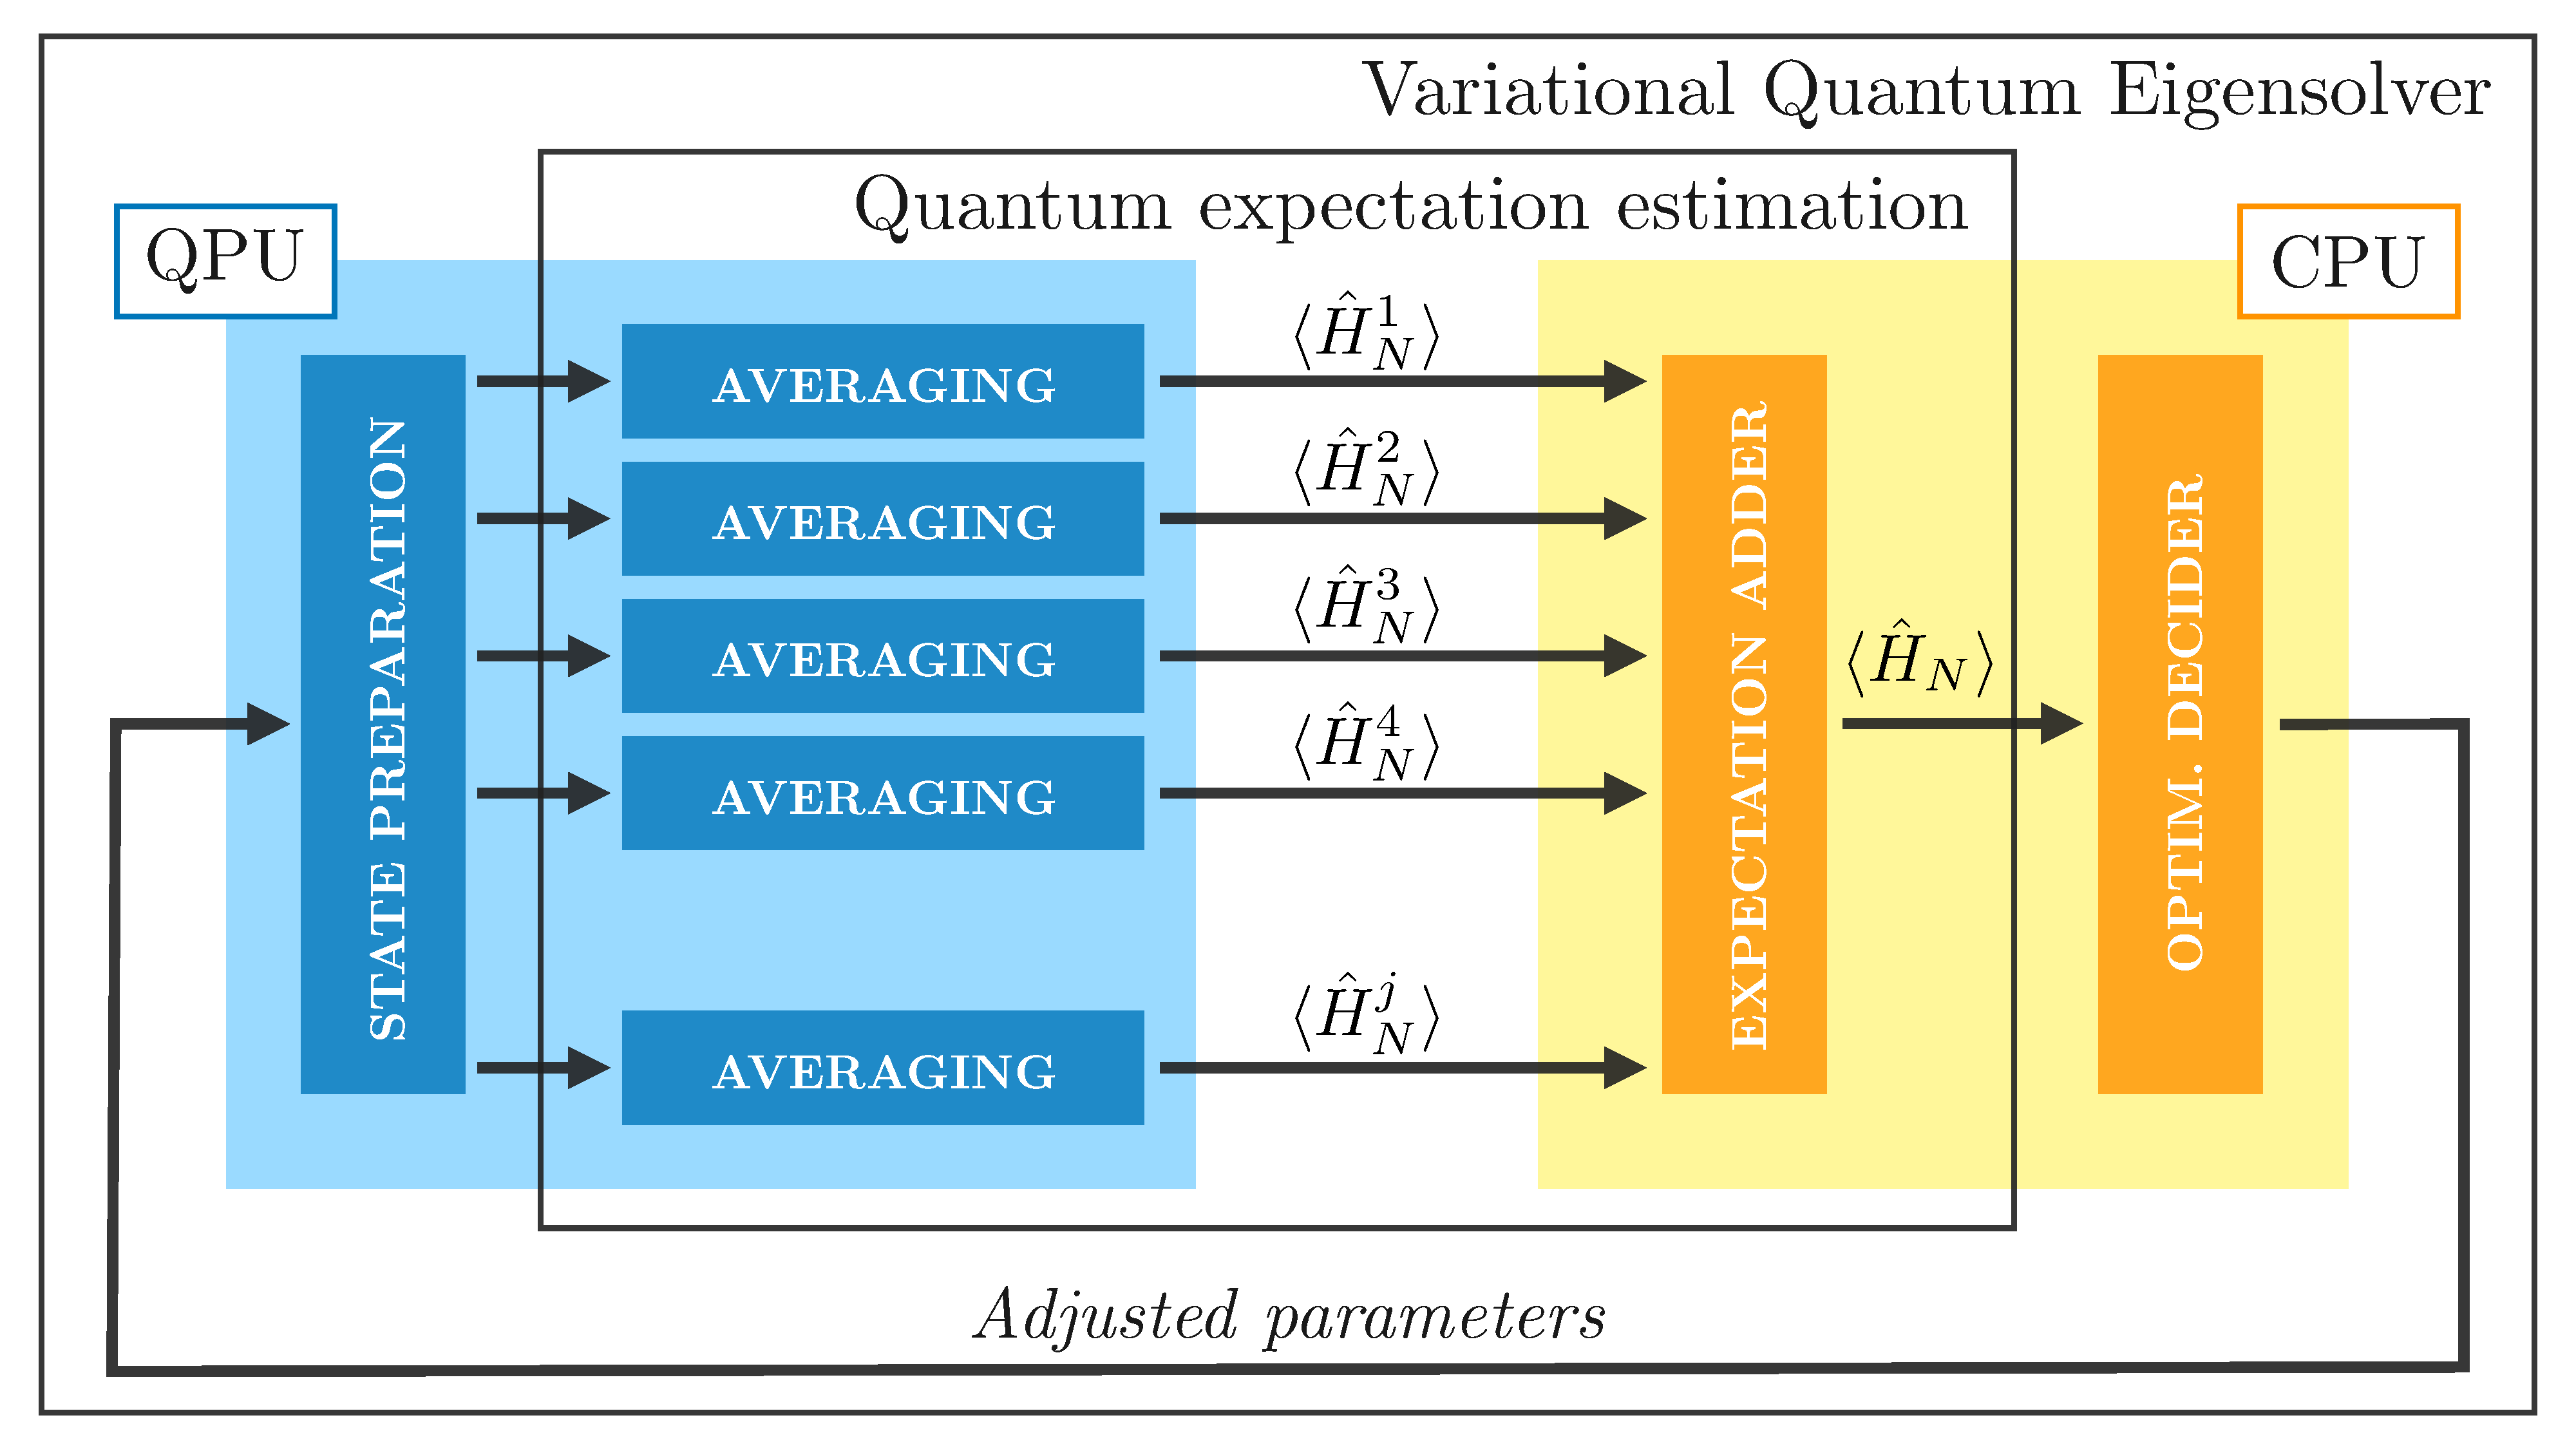
\includegraphics[width=.7\paperwidth]{Figures/chapter05/VQE}
	\end{center}

\end{frame}

%% ----------------------------------------------------------------------------
%% ----------------------------------------------------------------------------

\begin{frame}[allowframebreaks]{Subspace-search VQE (SSVQE)}

  Despite its success, VQE presents significant shortcomings that we would like to fix:

  \begin{itemize}
    \item<2-> Only prepare the minimum and maximum eigenstates of any given observable without having to modify it.
    \item<3-> Even if we were able to efficiently modify the observable to get other eigenstates, we would only be able to prepare one of those states at a time.
    \item<4-> Real-world problems require us to know not only the ground state, but also a number of relevant excited states.
  \end{itemize}

%% ----------------------------------------------------------------------------
\break
%% ----------------------------------------------------------------------------

  \textbf{Subspace-search VQE} can be summarized as:

  \begin{itemize}
    \item Construct an ansatz circuit $U(\theta)$ and choose input states $\qty{\ket{\varphi_j}}_{j=0}^{k}$ which are orthogonal with each other: $\braket{\varphi_i}{\varphi_j} =  \delta_{ij}$.
    \item Choose arbitrary weights so that $w_i > w_j$ if $i < j$, and minimize:
    \begin{gather*}
      \mathcal{L}_w(\theta) \defeq \sum_{j = 0}^{k} w_j \mel{\varphi_j}{U^\dagger(\theta) H U(\theta)}{\varphi_j} \qd
    \end{gather*}
  \end{itemize}

  Defining $\theta^*$ as the set of parameters that minimizes $\mathcal{L}_w(\theta)$, the ground state $\ket{\phi_{0}}$, and $k$ first excited states $\qty{\ket{\phi_{j}}}_{j=1}^k$ (in order) are approximated by:

  \begin{gather*}
    \ket{\phi_j} \cong U(\theta^*) \ket{\varphi_j} \qd
  \end{gather*}

  The catch with this algorithm is that it often requires a larger number of parameters and certain degree of redundancy in the way we prepare quantum states.

\end{frame}

%%    _____  _____
%%   |  __ \|  __ \    AUTHOR: Pedro Rivero
%%   | |__) | |__) |   ---------------------------------
%%   |  ___/|  _  /    DATE: November 10, 2021
%%   | |    | | \ \    ---------------------------------
%%   |_|    |_|  \_\   https://github.com/pedrorrivero
%%

\section{Solving NJL}

%% ----------------------------------------------------------------------------
%% ----------------------------------------------------------------------------

\begin{frame}[allowframebreaks]{Quantum computing the NJL model}

  \begin{itemize}
    \item<1-> Since we would like to study both the ground state, as well as the first excited hadron state in NJL, we will be using SSVQE as our variational algorithm.
    \item<2-> Using HVA we can use the fact that adiabatic state preparation maps corresponding excited states, to raise our chances of getting the correct output eigenstates in SSVQE without need for redundancy.
    \item<3-> HVA's parametrization is based on the system's Hamiltonian, it will share its symmetries. This means that we can easily use SSVQE to get non-consecutive output eigenstates by simply using non-consecutive initial eigenstates.
    \item<4-> HVA requires breaking up our Hamiltonian into its non-commuting components.
  \end{itemize}


%% ----------------------------------------------------------------------------
\break
%% ----------------------------------------------------------------------------

  \begin{align*}
    H_{N}^{(1)} \quad\defeq\quad&
      \frac{1}{4a} \sum_\alpha \sum_{n=\text{even}}^{2N-1}
      \qty[
        \sigma_\alpha^{1}(n+1) \sigma_\alpha^{2}(n) -
        \sigma_\alpha^{2}(n+1) \sigma_\alpha^{1}(n)
      ] \qc\\
    H_{N}^{(2)} \quad\defeq\quad& - \frac{G_{\pi}}{2a} \sum_{n=0}^{N-1} \qty[
      \sum_{\alpha} \dbtilde{H}_{N}^{\alpha\alpha}(n) + 2
      \sum_{\alpha < \beta} \dbtilde{H}_{N}^{\alpha\beta}(n)] \qc\\
    H_{N}^{(3)} \quad\defeq\quad&
      \frac{1}{4a} \sum_\alpha \sum_{n=\text{odd}}^{2N-2}
      \qty[
        \sigma_\alpha^{1}(n+1) \sigma_\alpha^{2}(n) -
        \sigma_\alpha^{2}(n+1) \sigma_\alpha^{1}(n)
      ] + \nonumber\\&
      \frac{1}{4a} \sum_\alpha \!
      \qty[\prod_{l=1}^{2N-2} \!\! \sigma_\alpha^3(l)] \!
      \qty[
        \sigma_\alpha^{1}(0) \sigma_\alpha^{2}(2N \!-\! 1) -
        \sigma_\alpha^{2}(0) \sigma_\alpha^{1}(2N \!-\! 1)
      ] \qc\\
    H_{N}^{(4)} \quad\defeq\quad&
      \frac{m}{2} \sum_\alpha \sum_{n=0}^{2N-1}
      (-1)^{n+1}\sigma_\alpha^{3}(n) \qc
  \end{align*}

%% ----------------------------------------------------------------------------
\break
%% ----------------------------------------------------------------------------

  \begin{minipage}[c]{\linewidth}\begin{multicols}{2}

    We choose the mass term for the initial states:

    \begin{gather*}
      H_{N}^{(4)} \;\defeq\;
        \frac{m}{2} \sum_\alpha \sum_{n=0}^{2N-1}
        (-1)^{n+1}\sigma_\alpha^{3}(n)
    \end{gather*}

    \begin{itemize}
      \item<1-> Ground: $\ket{\Omega_0} \defeq \ket{\bin...1010101010}$
      \item<1-> Hadron: $\ket{h_0} \defeq \ket{\bin...1010101001} + \cdots$
    \end{itemize}

    Where we can build the initial hadron state by implementing \textbf{Dicke states}:

    \begin{center}
      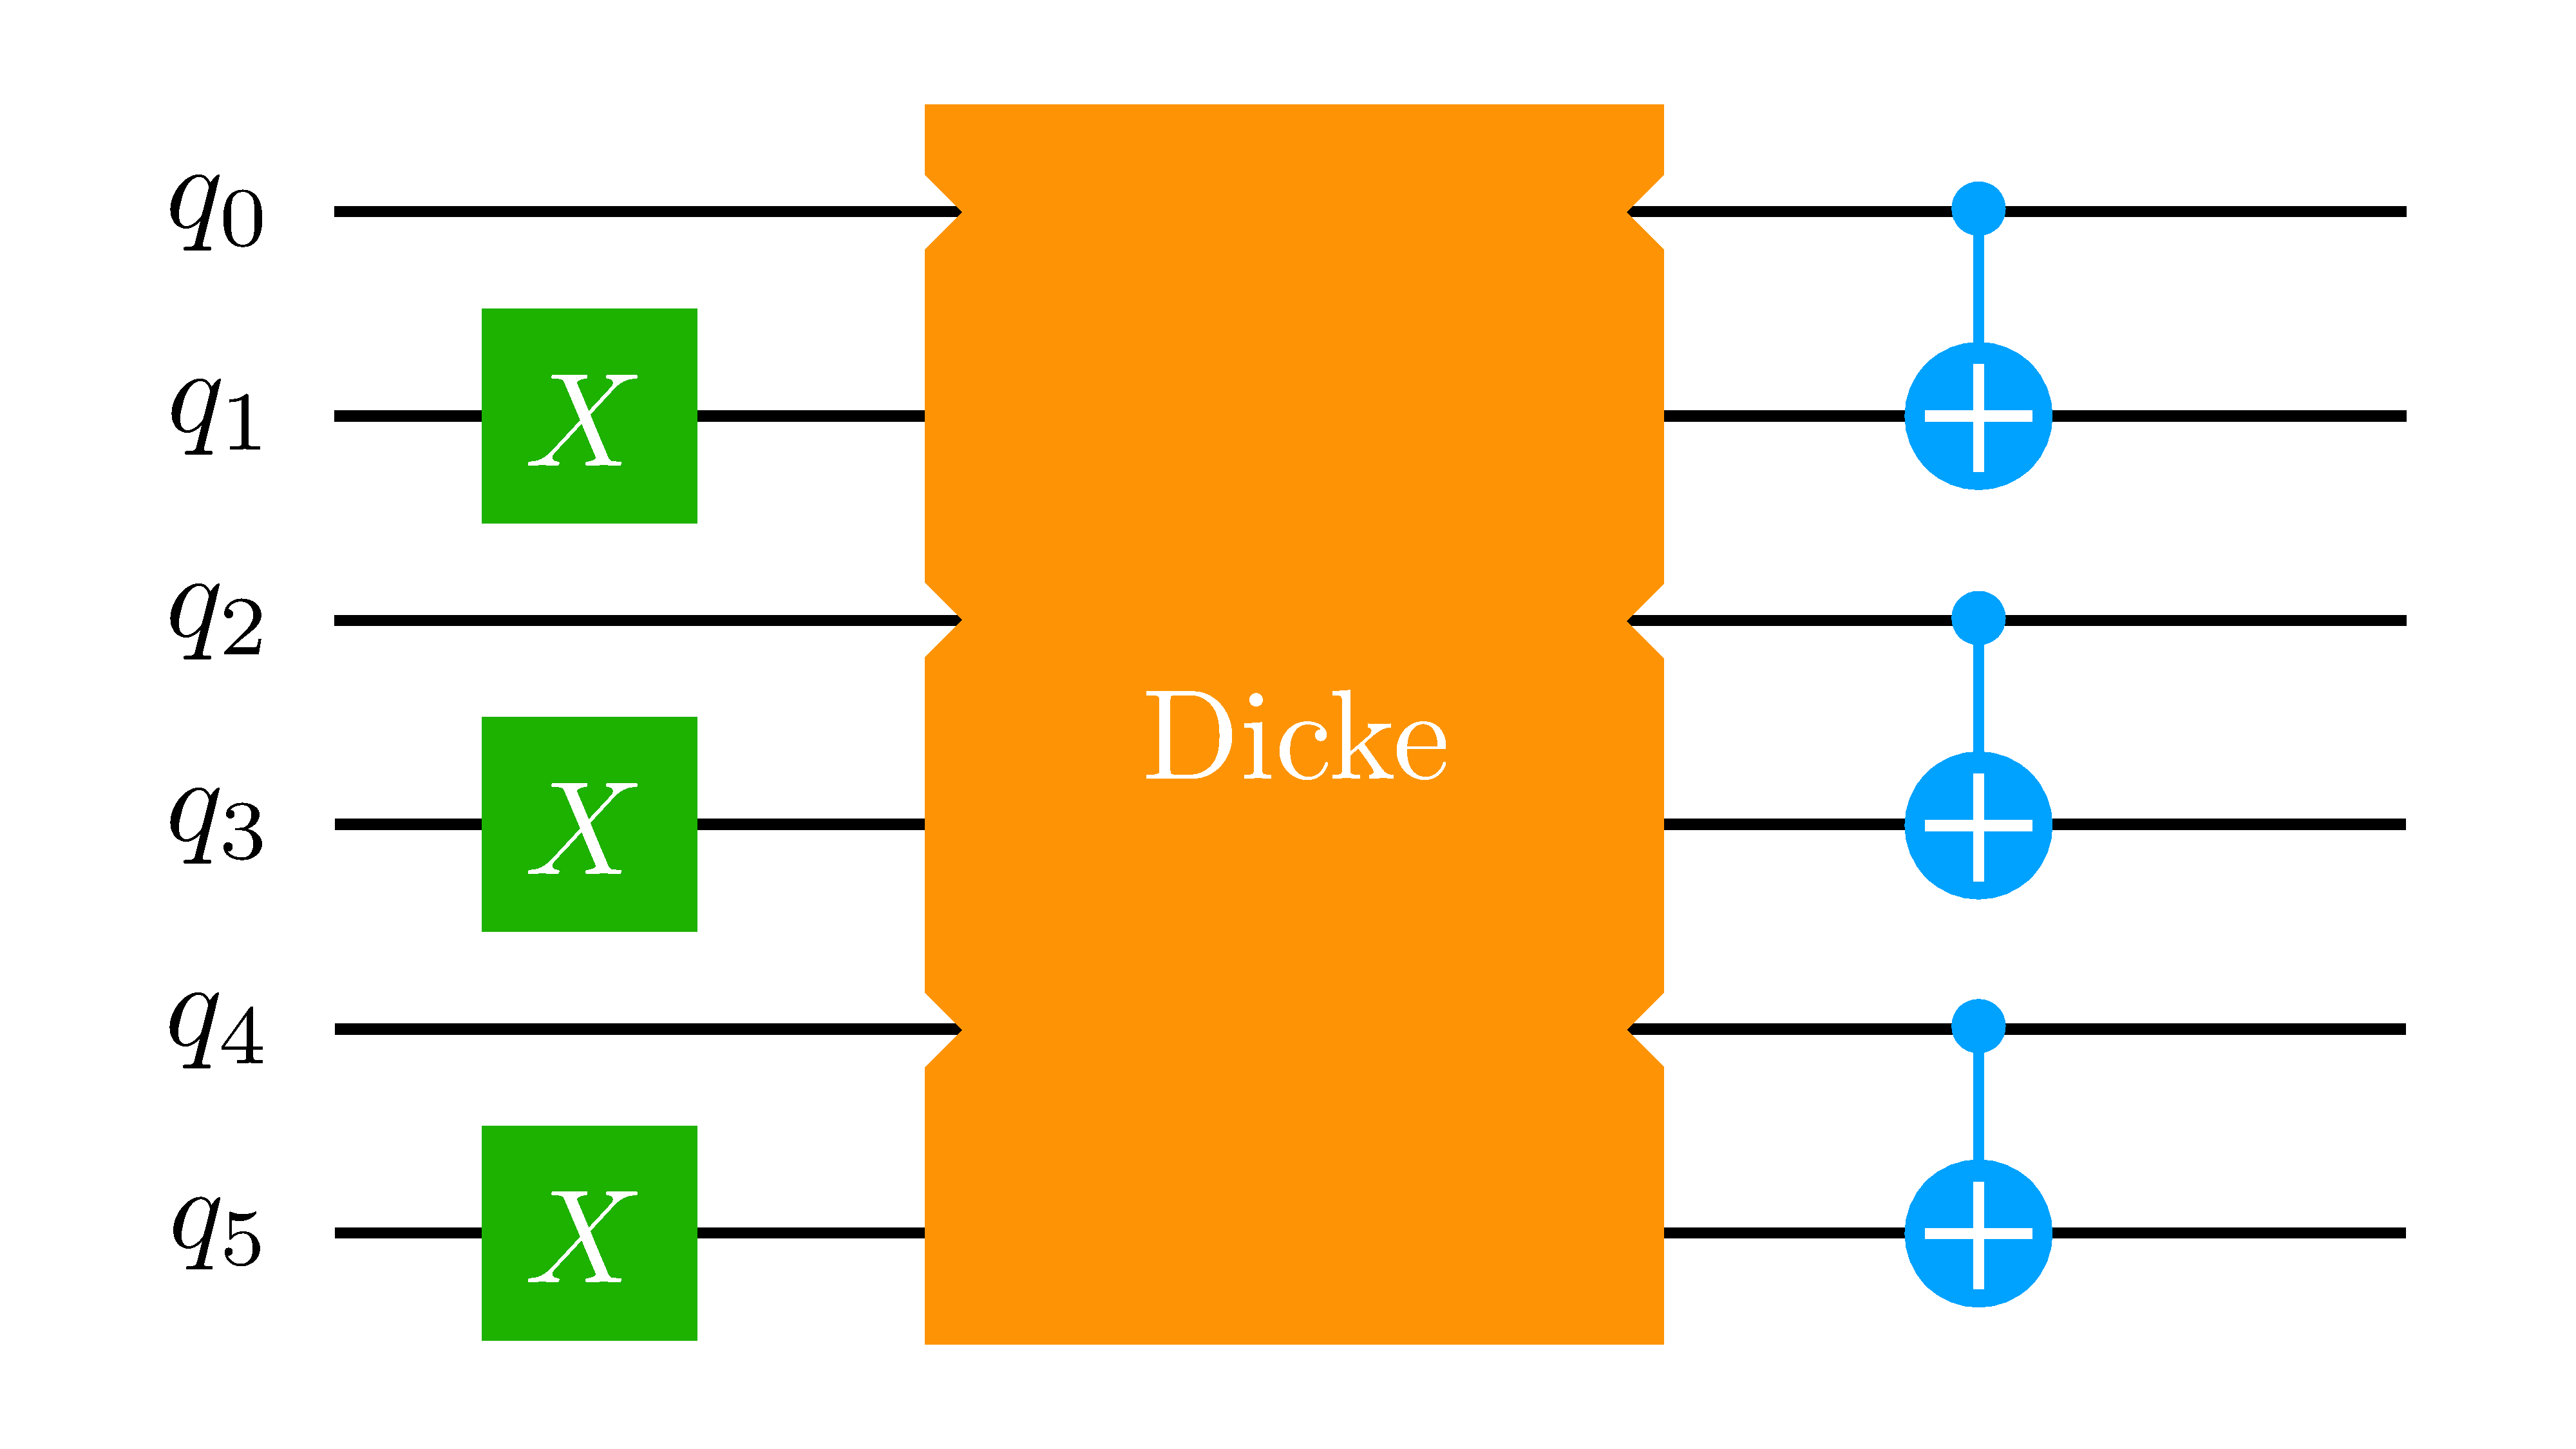
\includegraphics[width=.25\paperwidth]{Figures/chapter06/hadron-init}
    \end{center}

    \vfill
    \columnbreak

    \begin{center}
      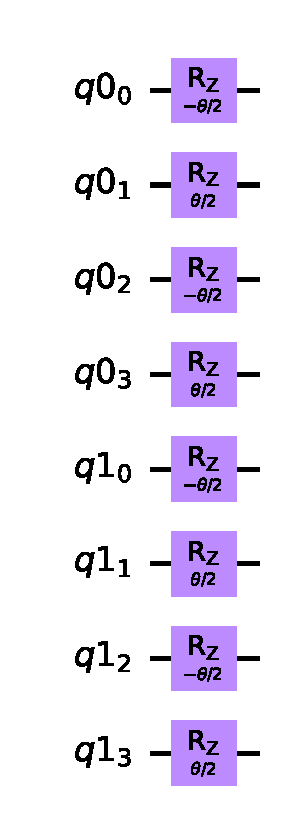
\includegraphics[width=.15\paperwidth]{Figures/chapter06/H4-rotation}
    \end{center}

  \end{multicols}\end{minipage}

%% ----------------------------------------------------------------------------
\break\break
%% ----------------------------------------------------------------------------

  \begin{minipage}[c]{\linewidth}
  \begin{gather*}
    H_{N}^{(2)} \;\defeq\; - \frac{G_{\pi}}{2a} \sum_{n=0}^{N-1} \qty[
      \sum_{\alpha} \dbtilde{H}_{N}^{\alpha\alpha}(n) + 2
      \sum_{\alpha < \beta} \dbtilde{H}_{N}^{\alpha\beta}(n)] \\
    \dbtilde{H}_{N}^{\alpha\beta}(n) \qra
    \frac{1}{4} \sum_{{j=0}\atop{k=0}}^{1}
    (-1)^{j+k} \, \sigma_\alpha^{3}(2n+j) \, \sigma_\beta^{3}(2n+k) \
  \end{gather*}
  \vspace{-2em}
  \begin{center}
    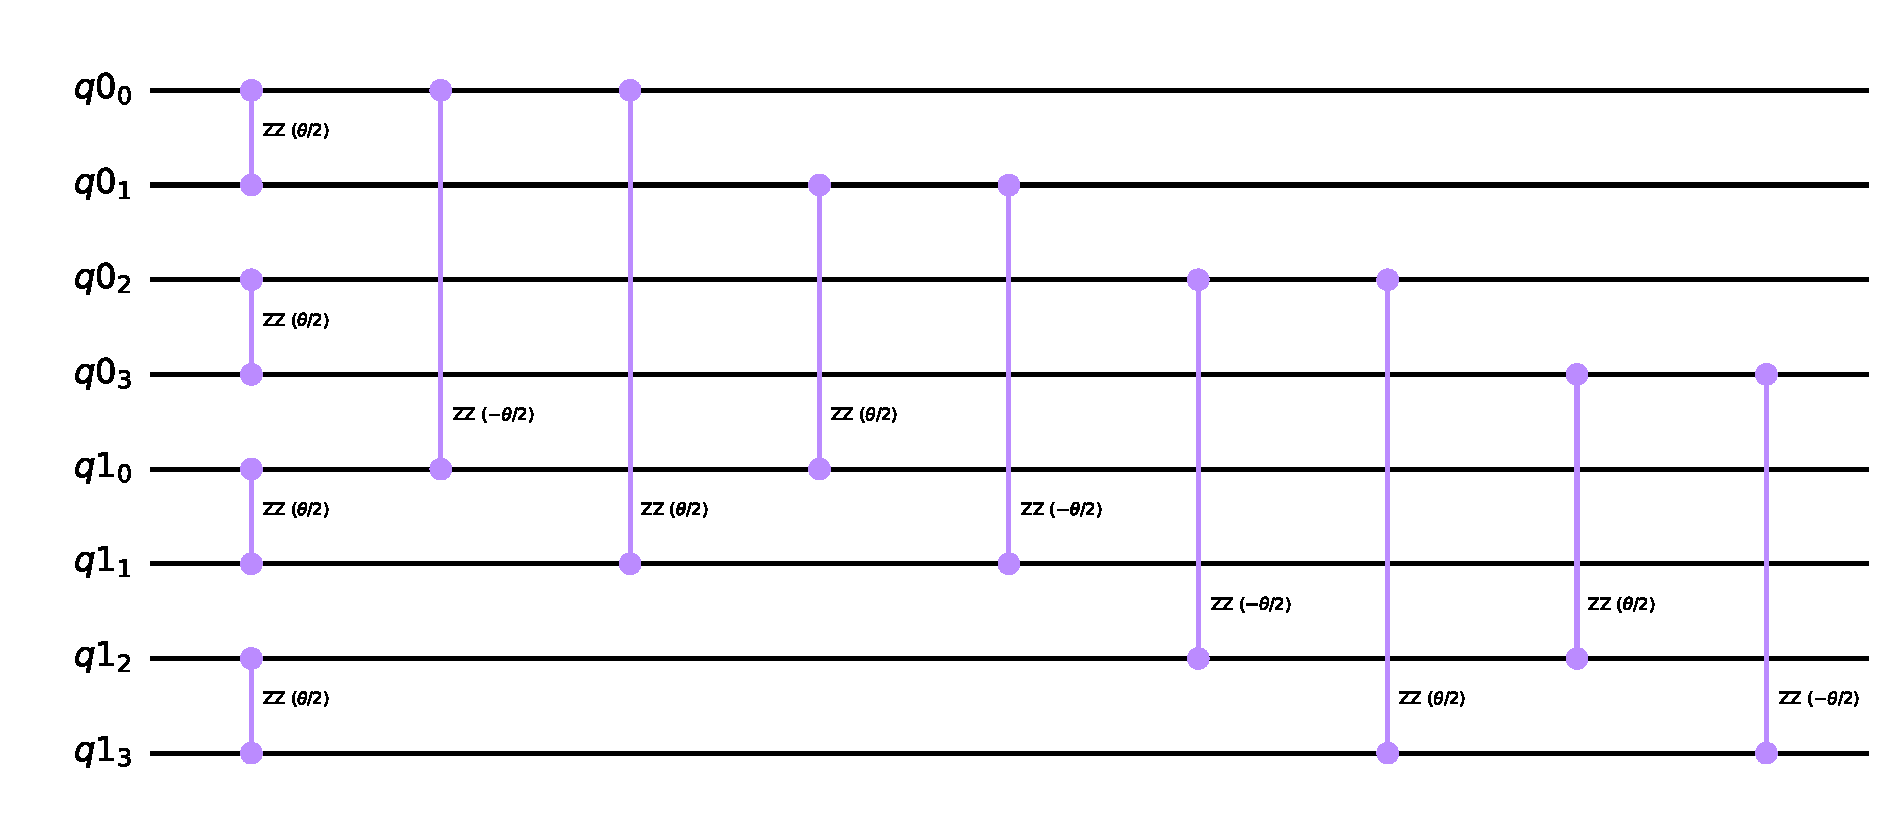
\includegraphics[width=.60\paperwidth]{Figures/chapter06/H2-rotation}
  \end{center}
  \vspace{-2em}
\end{minipage}


%% ----------------------------------------------------------------------------
\break
%% ----------------------------------------------------------------------------

  The kinetic terms of the form $XY-YX$ can be easily exponentiated by noting that:

  \begin{multicols}{2}

    \begin{gather*}
      \frac{1}{2}(X_1Y_0 - Y_1X_0) =
      \mqty[\phpl 0 & \phpl 0 & \phpl 0 & \phpl 0 \\
            \phpl 0 & \phpl 0 & \phpl i & \phpl 0 \\
            \phpl 0 &      -i & \phpl 0 & \phpl 0 \\
            \phpl 0 & \phpl 0 & \phpl 0 & \phpl 0   ] \qc
    \end{gather*}

    \begin{itemize}
      \item Zero eigenvalue on even parity states: single particle/antiparticle states
      \item Pauli~Y in the subspace $\qty{\ket{\bin 10}, \ket{\bin 01}}$: creates and annihilates particle-antiparticle pairs.
    \end{itemize}

  \columnbreak

    \begin{center}
      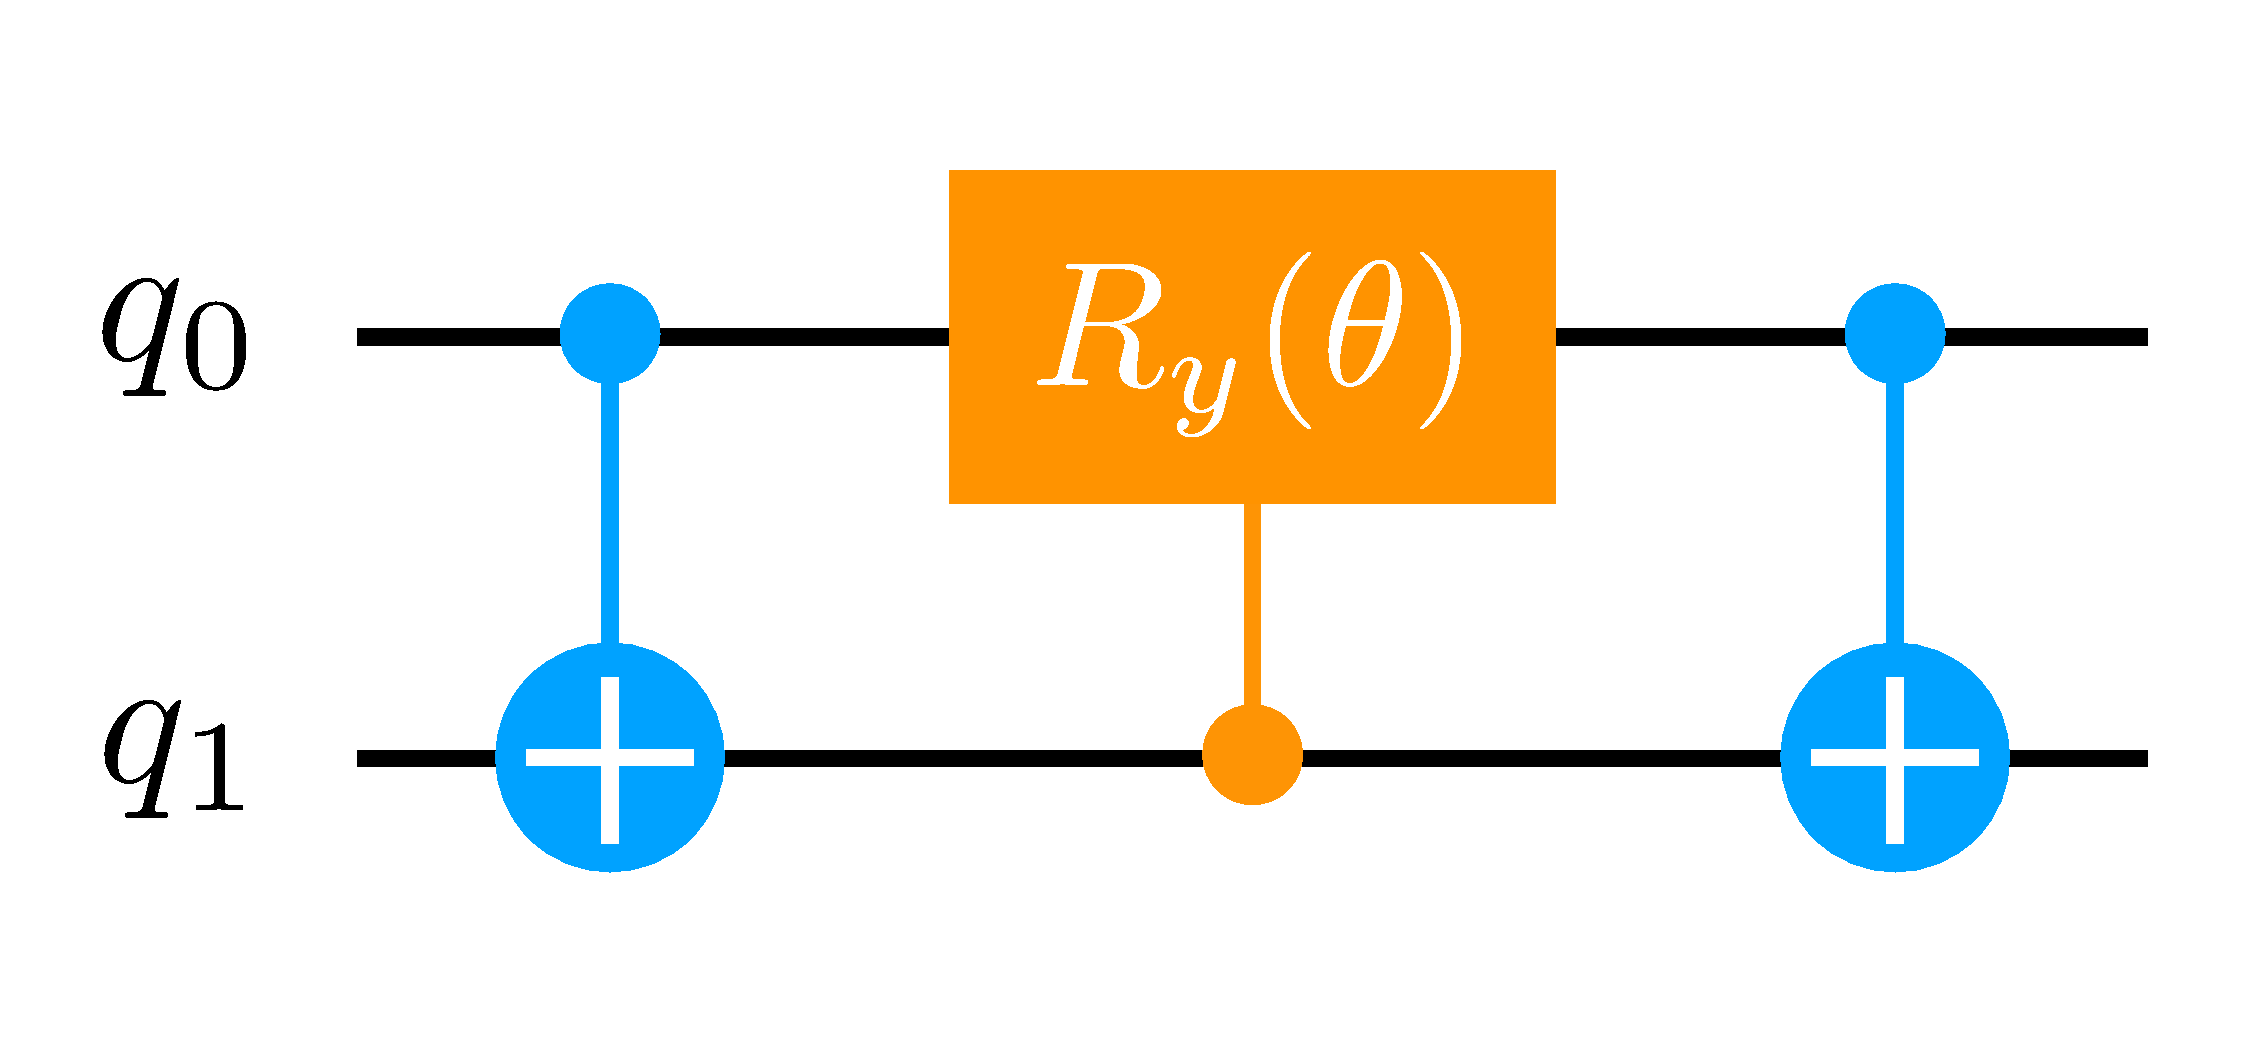
\includegraphics[width=.25\paperwidth]{Figures/chapter06/xy-rotation}
    \end{center}

    \begin{center}
      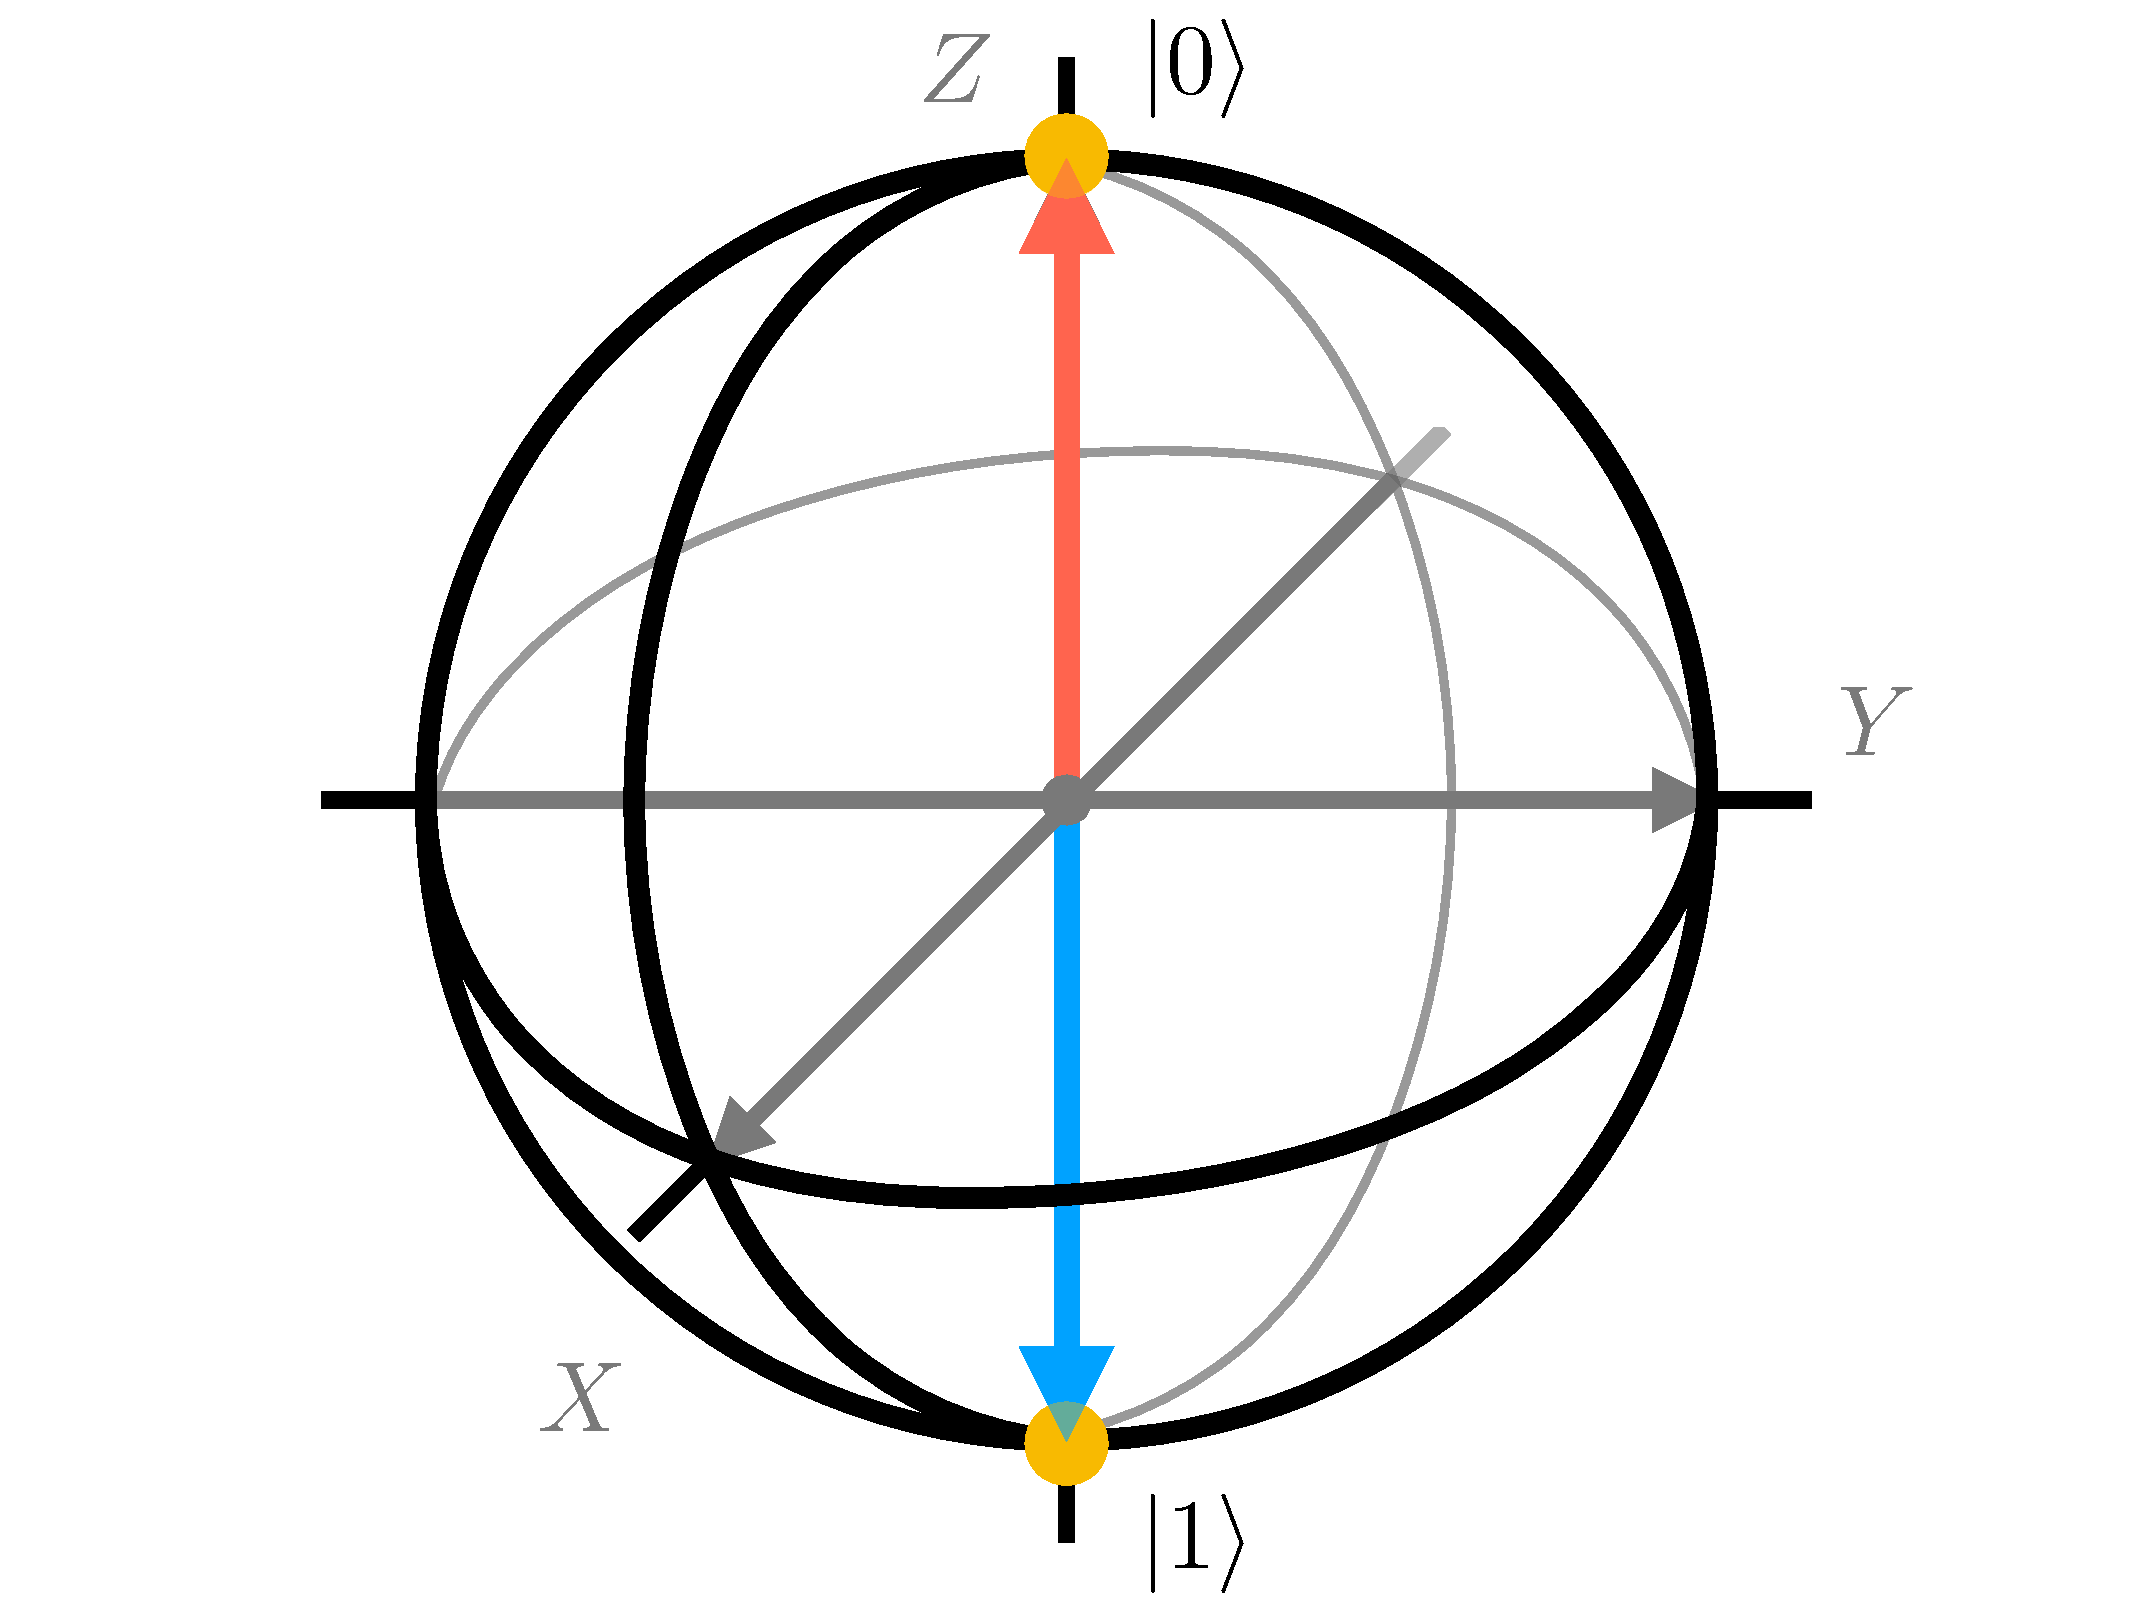
\includegraphics[width=.25\paperwidth]{Figures/chapter01/bloch-sphere}
    \end{center}

  \end{multicols}

  % which means that it acts with zero eigenvalue on even parity states, and as Pauli~Y in the subspace $\qty{\ket{\bin 10}, \ket{\bin 01}}$. As we will see, this implies that the evolution associated to the kinetic term can only create or annihilate particle-antiparticle pairs on a single physical site (i.e. $H_N^{(1)}$), or between nearest neighbors (i.e. $H_N^{(3)}$); enabling motion along the lattice, and hinting at a necessary number of rotations being proportional to the number of physical lattice sites (i.e. to allow pairs to completely cycle around the lattice), which in turn implies an efficient polynomial parametrization of Hilbert space. Moreover, it also ensures that single-particle states are unreachable and therefore charge is conserved, which is consistent with all that we know about QCD. The boundary term with the string will be similar but rotating on $\qty(\bigotimes Z) Y$ instead of just on $Y$.

%% ----------------------------------------------------------------------------
\break
%% ----------------------------------------------------------------------------

  \begin{minipage}[c]{\linewidth}
  \vspace{-1em}
  \footnotesize{\begin{align*}
    H_{N}^{(1)} \;\defeq\;&
      \frac{1}{4a} \sum_\alpha \sum_{n=\text{even}}^{2N-1}
      \qty[
        \sigma_\alpha^{1}(n+1) \sigma_\alpha^{2}(n) -
        \sigma_\alpha^{2}(n+1) \sigma_\alpha^{1}(n)
      ] \qc\\
    H_{N}^{(3)} \;\defeq\;&
      \frac{1}{4a} \sum_\alpha \sum_{n=\text{odd}}^{2N-2}
      \qty[
        \sigma_\alpha^{1}(n+1) \sigma_\alpha^{2}(n) -
        \sigma_\alpha^{2}(n+1) \sigma_\alpha^{1}(n)
      ] +\\&
      \frac{1}{4a} \sum_\alpha \!
      \qty[\prod_{l=1}^{2N-2} \!\! \sigma_\alpha^3(l)] \!
      \qty[
        \sigma_\alpha^{1}(0) \sigma_\alpha^{2}(2N \!-\! 1) -
        \sigma_\alpha^{2}(0) \sigma_\alpha^{1}(2N \!-\! 1)
      ]
  \end{align*}}
  \vspace{-1em}
  \begin{figure}[!p]
  	\centering
  	\begin{minipage}[c]{.20\linewidth}
  		\centering
  		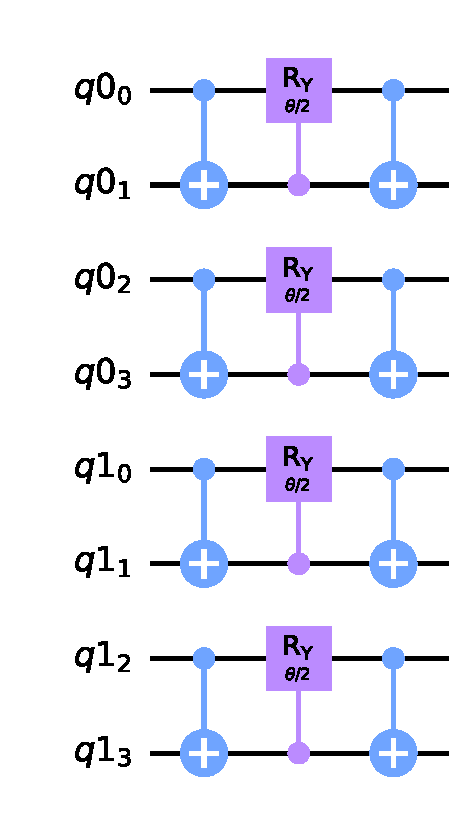
\includegraphics[height=15em]{Figures/chapter06/H1-rotation}
  	\end{minipage}
  	\hspace{1em}
  	\begin{minipage}[c]{.50\linewidth}
  		\centering
  		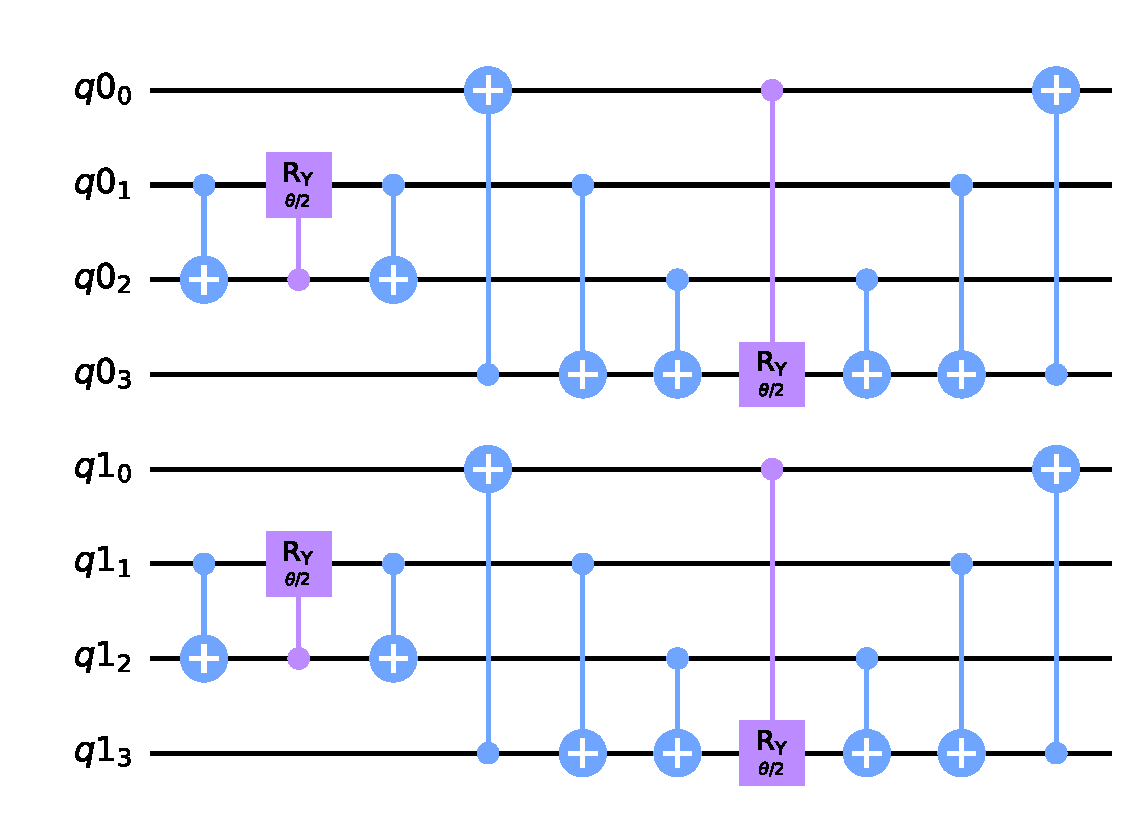
\includegraphics[height=15em]{Figures/chapter06/H3-rotation}
  	\end{minipage}
  \end{figure}
  \vspace{-2em}
  \end{minipage}


\end{frame}

%% ----------------------------------------------------------------------------
%% ----------------------------------------------------------------------------

\subsection{Ground/hadron states}

%% ----------------------------------------------------------------------------
%% ----------------------------------------------------------------------------

\begin{frame}{Ground and hadron states ($N=3$, $N_\text{flavor}=2$)}

  \begin{figure}[!p]
  	\centering
  	\begin{minipage}[c]{.40\linewidth}
  		\centering
  		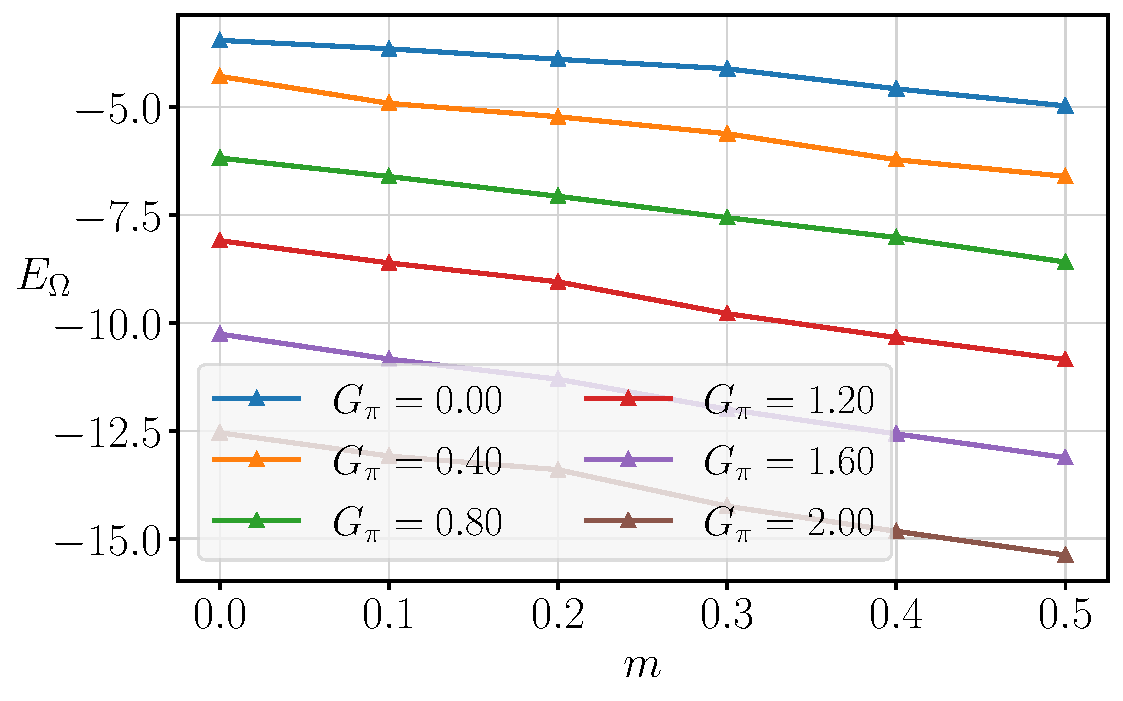
\includegraphics[width=\linewidth]{Figures/chapter06/g-Ev-curves}
  	\end{minipage}
    \hspace{.025\linewidth}
  	\begin{minipage}[c]{.40\linewidth}
  		\centering
  		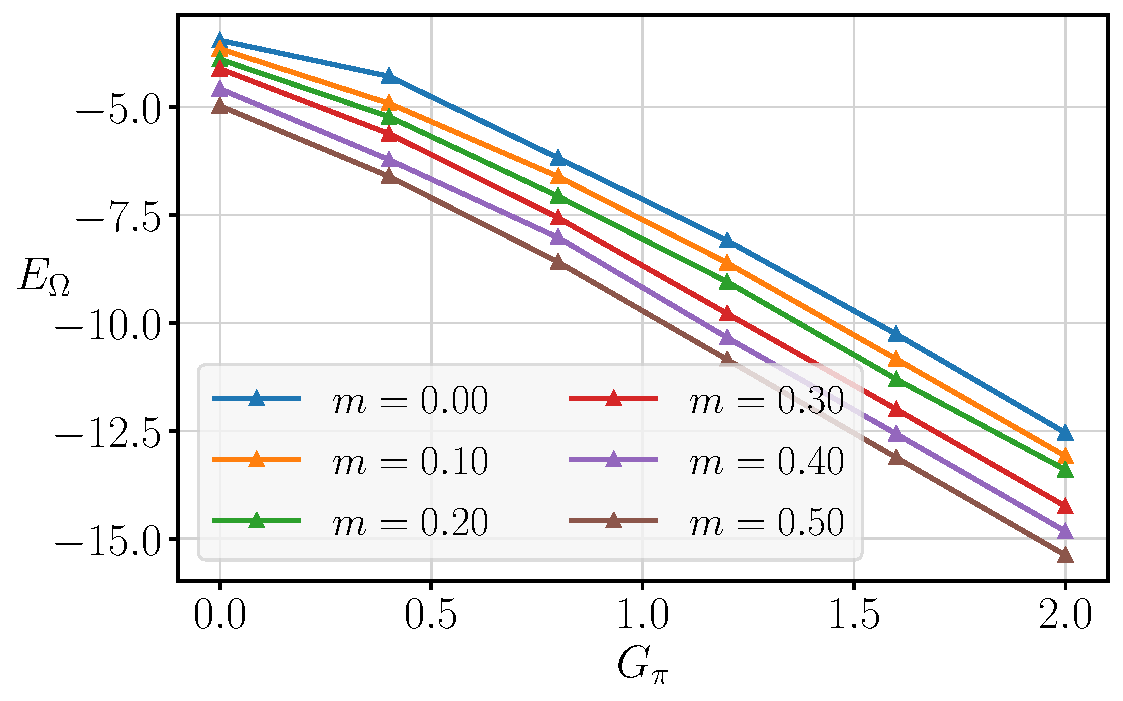
\includegraphics[width=\linewidth]{Figures/chapter06/m-Ev-curves}
  	\end{minipage}
  \end{figure}

  \begin{figure}[!p]
  	\centering
  	\begin{minipage}[c]{.40\linewidth}
  		\centering
  		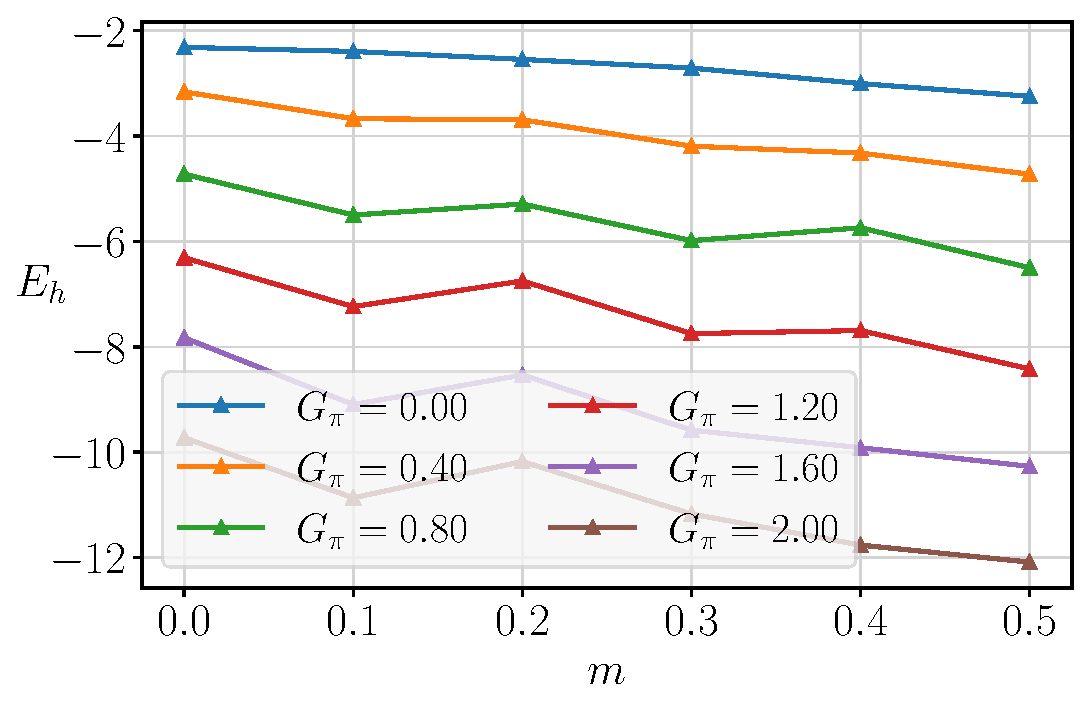
\includegraphics[width=\linewidth]{Figures/chapter06/g-Eh-curves}
  	\end{minipage}
    \hspace{.025\linewidth}
  	\begin{minipage}[c]{.40\linewidth}
  		\centering
  		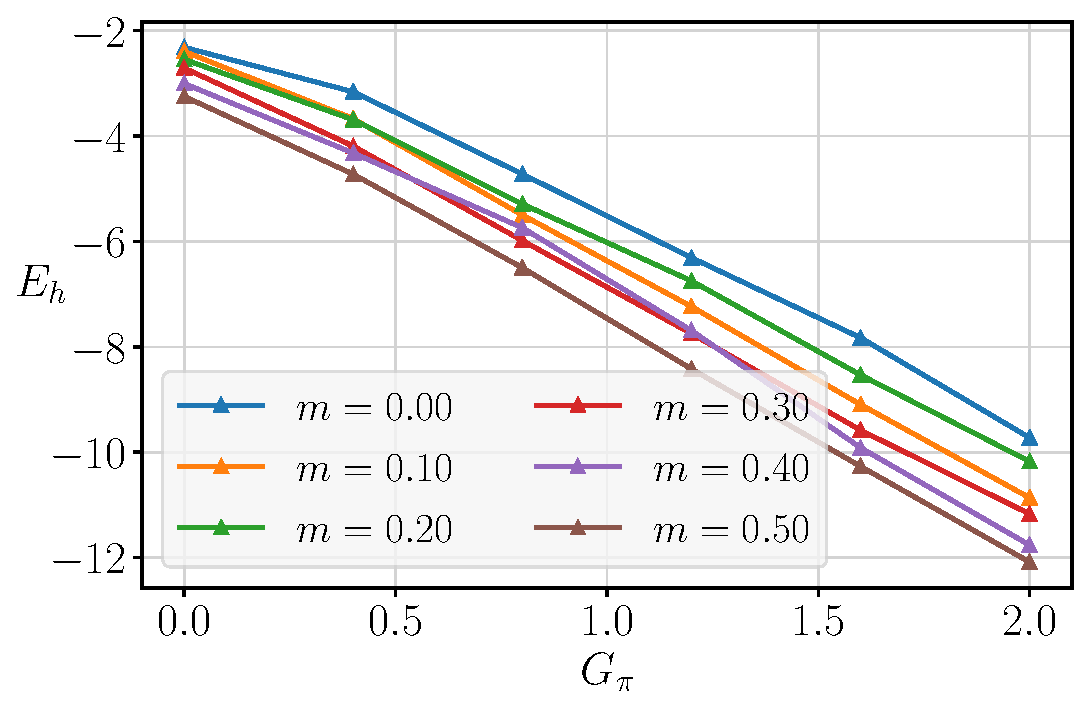
\includegraphics[width=\linewidth]{Figures/chapter06/m-Eh-curves}
  	\end{minipage}
  \end{figure}

\end{frame}
%% ----------------------------------------------------------------------------
%% ----------------------------------------------------------------------------

\subsection{Mass generation}

%% ----------------------------------------------------------------------------
%% ----------------------------------------------------------------------------

\begin{frame}[allowframebreaks]{Mass generation ($N=3$, $N_\text{flavor}=2$)}

  With these results, we can now obtain the hadron's mass as the difference between the hadron's energy and the computed vacuum energy:

  \begin{gather*}
    M \defeq \mel{h}{H_N}{h} - \mel{\Omega}{H_N}{\Omega} \qd
  \end{gather*}

  \begin{figure}[!p]
  	\centering
  	\begin{minipage}[c]{.40\linewidth}
  		\centering
  		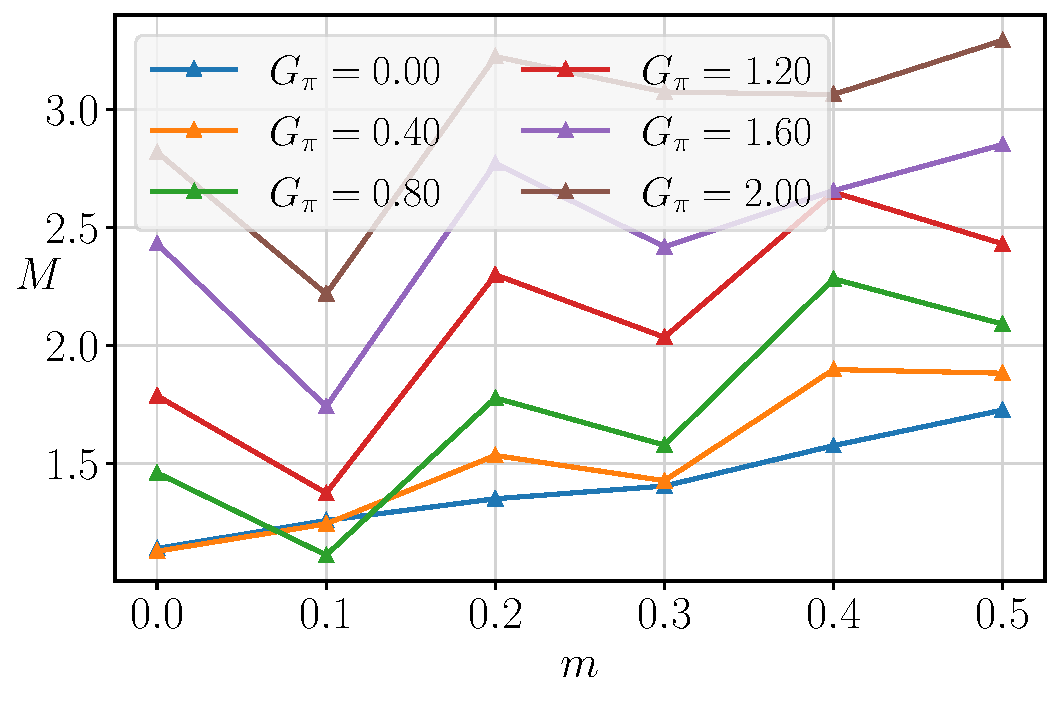
\includegraphics[width=\linewidth]{Figures/chapter06/g-mass-curves}
  	\end{minipage}
    \hspace{.025\linewidth}
  	\begin{minipage}[c]{.40\linewidth}
  		\centering
  		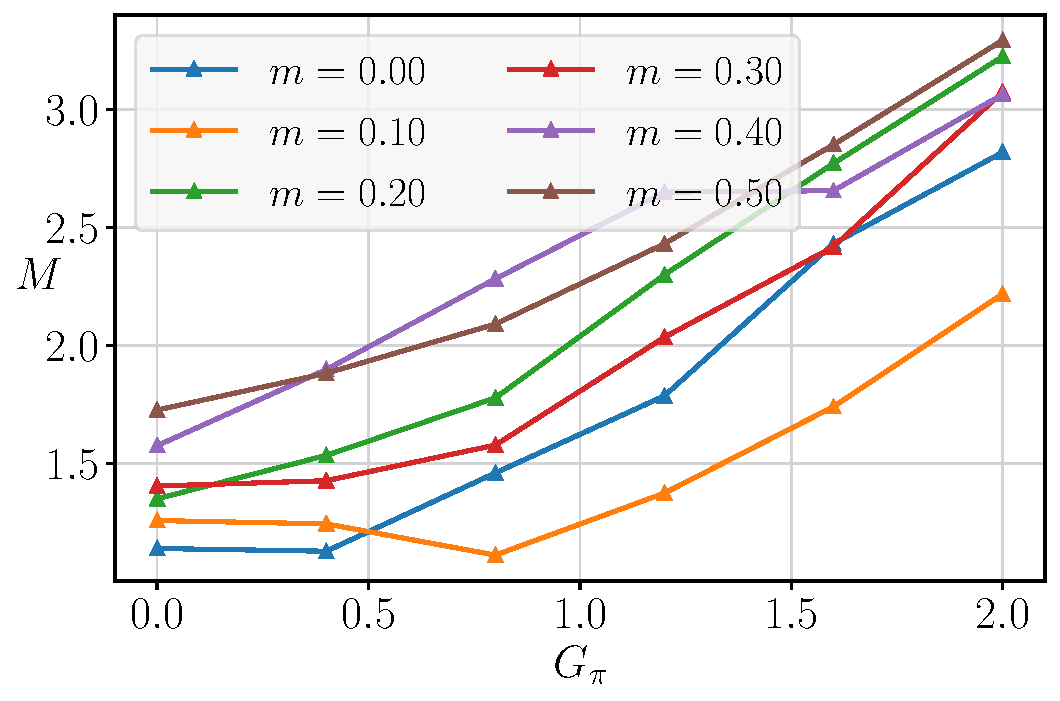
\includegraphics[width=\linewidth]{Figures/chapter06/m-mass-curves}
  	\end{minipage}
  \end{figure}

%% ----------------------------------------------------------------------------
\break
%% ----------------------------------------------------------------------------

  Nonetheless, we can see this more clearly by introducing a new metric. To motivate its definition, let us first define the different contributions to the mass of the hadron as:

  \begin{align*}
    M   \;\defeq\;&
      M_M + M_K + M_G \qc\\
    M_M \;\defeq\;&
      \mel{h}{H_N^{(M)}}{h} - \mel{\Omega}{H_N^{(M)}}{\Omega} \qc\\
    M_K \;\defeq\;&
      \mel{h}{H_N^{(K)}}{h} - \mel{\Omega}{H_N^{(K)}}{\Omega} \qc\\
    M_G \;\defeq\;&
      \mel{h}{H_N^{(G)}}{h} - \mel{\Omega}{H_N^{(G)}}{\Omega} \qd
  \end{align*}

  Our goal here is to compare the component of mass associated with interactions $M_G$, and that associated with the quark masses $M_M$. It is then natural to define:

  \begin{gather*}
    \mathcal{M}(m,G_\pi) \;\defeq\; \frac{M_G - M_M}{M} \qc
  \end{gather*}

%% ----------------------------------------------------------------------------
\break
%% ----------------------------------------------------------------------------

  From which we can distinguish three regimes:

  \begin{align*}
    M   \;\approx\;& M_G \qRa \mathcal{M} \approx +1 \qc\\
    M   \;\approx\;& M_M \qRa \mathcal{M} \approx -1 \qc\\
    M_G \;\approx\;& M_M \qRa \mathcal{M} \approx  0 \qd
  \end{align*}

  \begin{figure}[!tbp]
  	\centering
  	\begin{minipage}[c]{.40\linewidth}
  		\centering
  		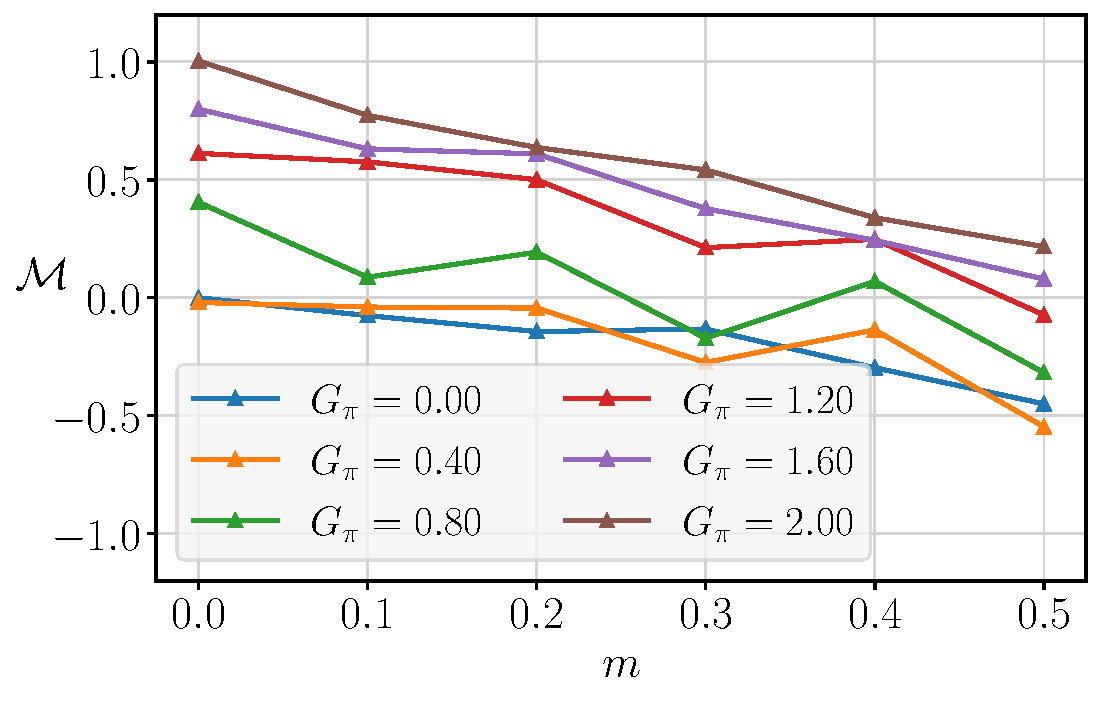
\includegraphics[width=\linewidth]{Figures/chapter06/g-ratio-curves}
  	\end{minipage}
    \hspace{.025\linewidth}
  	\begin{minipage}[c]{.40\linewidth}
  		\centering
  		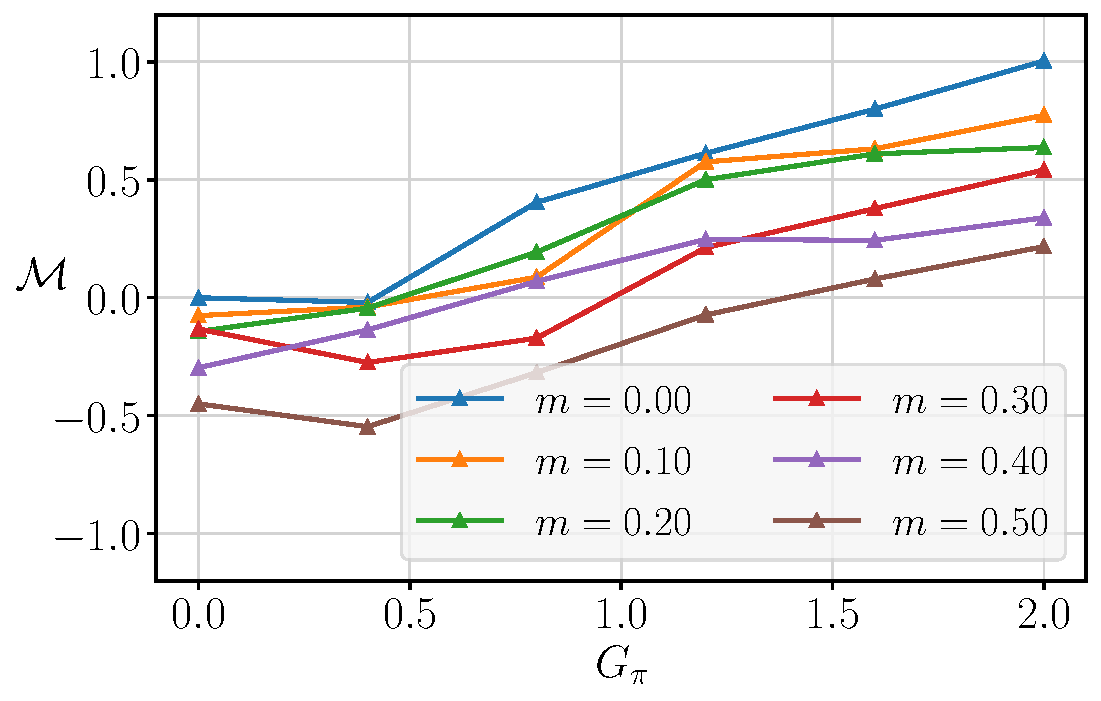
\includegraphics[width=\linewidth]{Figures/chapter06/m-ratio-curves}
  	\end{minipage}
  \end{figure}

\end{frame}

%%    _____  _____
%%   |  __ \|  __ \    AUTHOR: Pedro Rivero
%%   | |__) | |__) |   ---------------------------------
%%   |  ___/|  _  /    DATE: November 10, 2021
%%   | |    | | \ \    ---------------------------------
%%   |_|    |_|  \_\   https://github.com/pedrorrivero
%%

\section{QSR}

%% ----------------------------------------------------------------------------
%% ----------------------------------------------------------------------------

\begin{frame}[allowframebreaks]{Algorithm outline}

  \begin{minipage}[c]{\linewidth}
    \begin{center}
      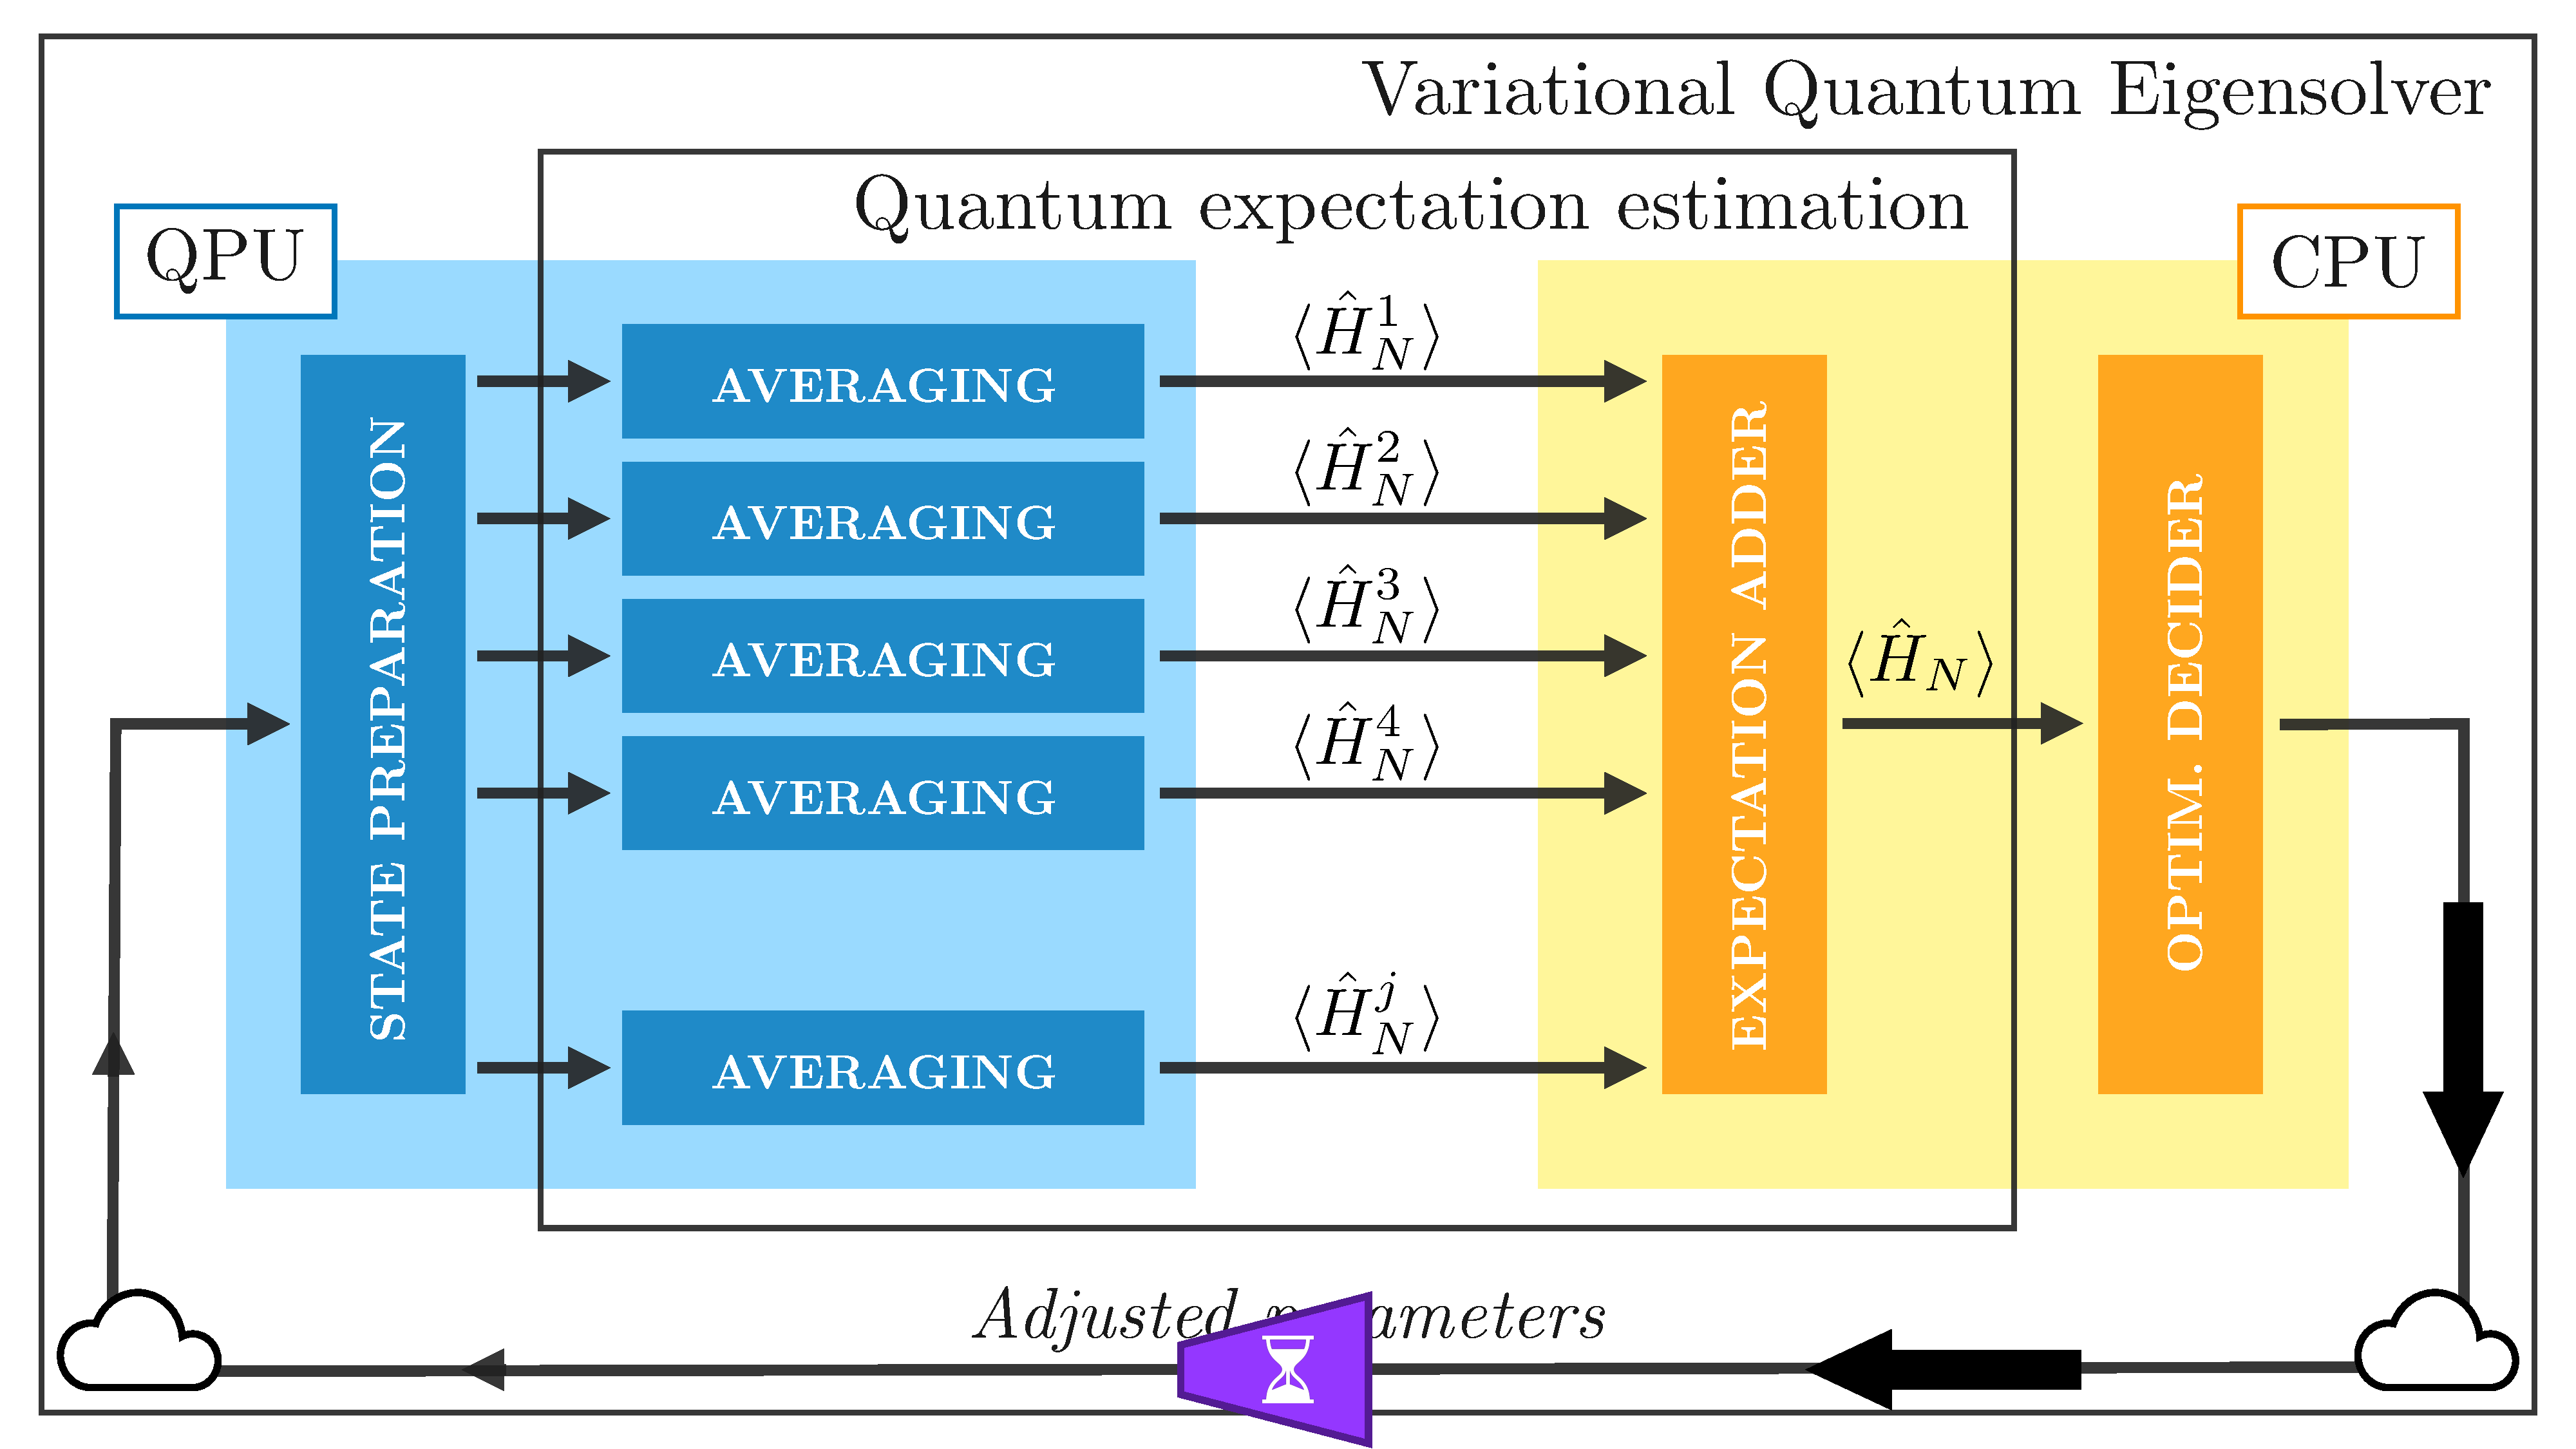
\includegraphics[width=.7\paperwidth]{Figures/VQE-bottleneck}
    \end{center}
  \end{minipage}

%% ----------------------------------------------------------------------------
\break
%% ----------------------------------------------------------------------------

  \begin{minipage}[c]{\linewidth}
    \begin{center}
      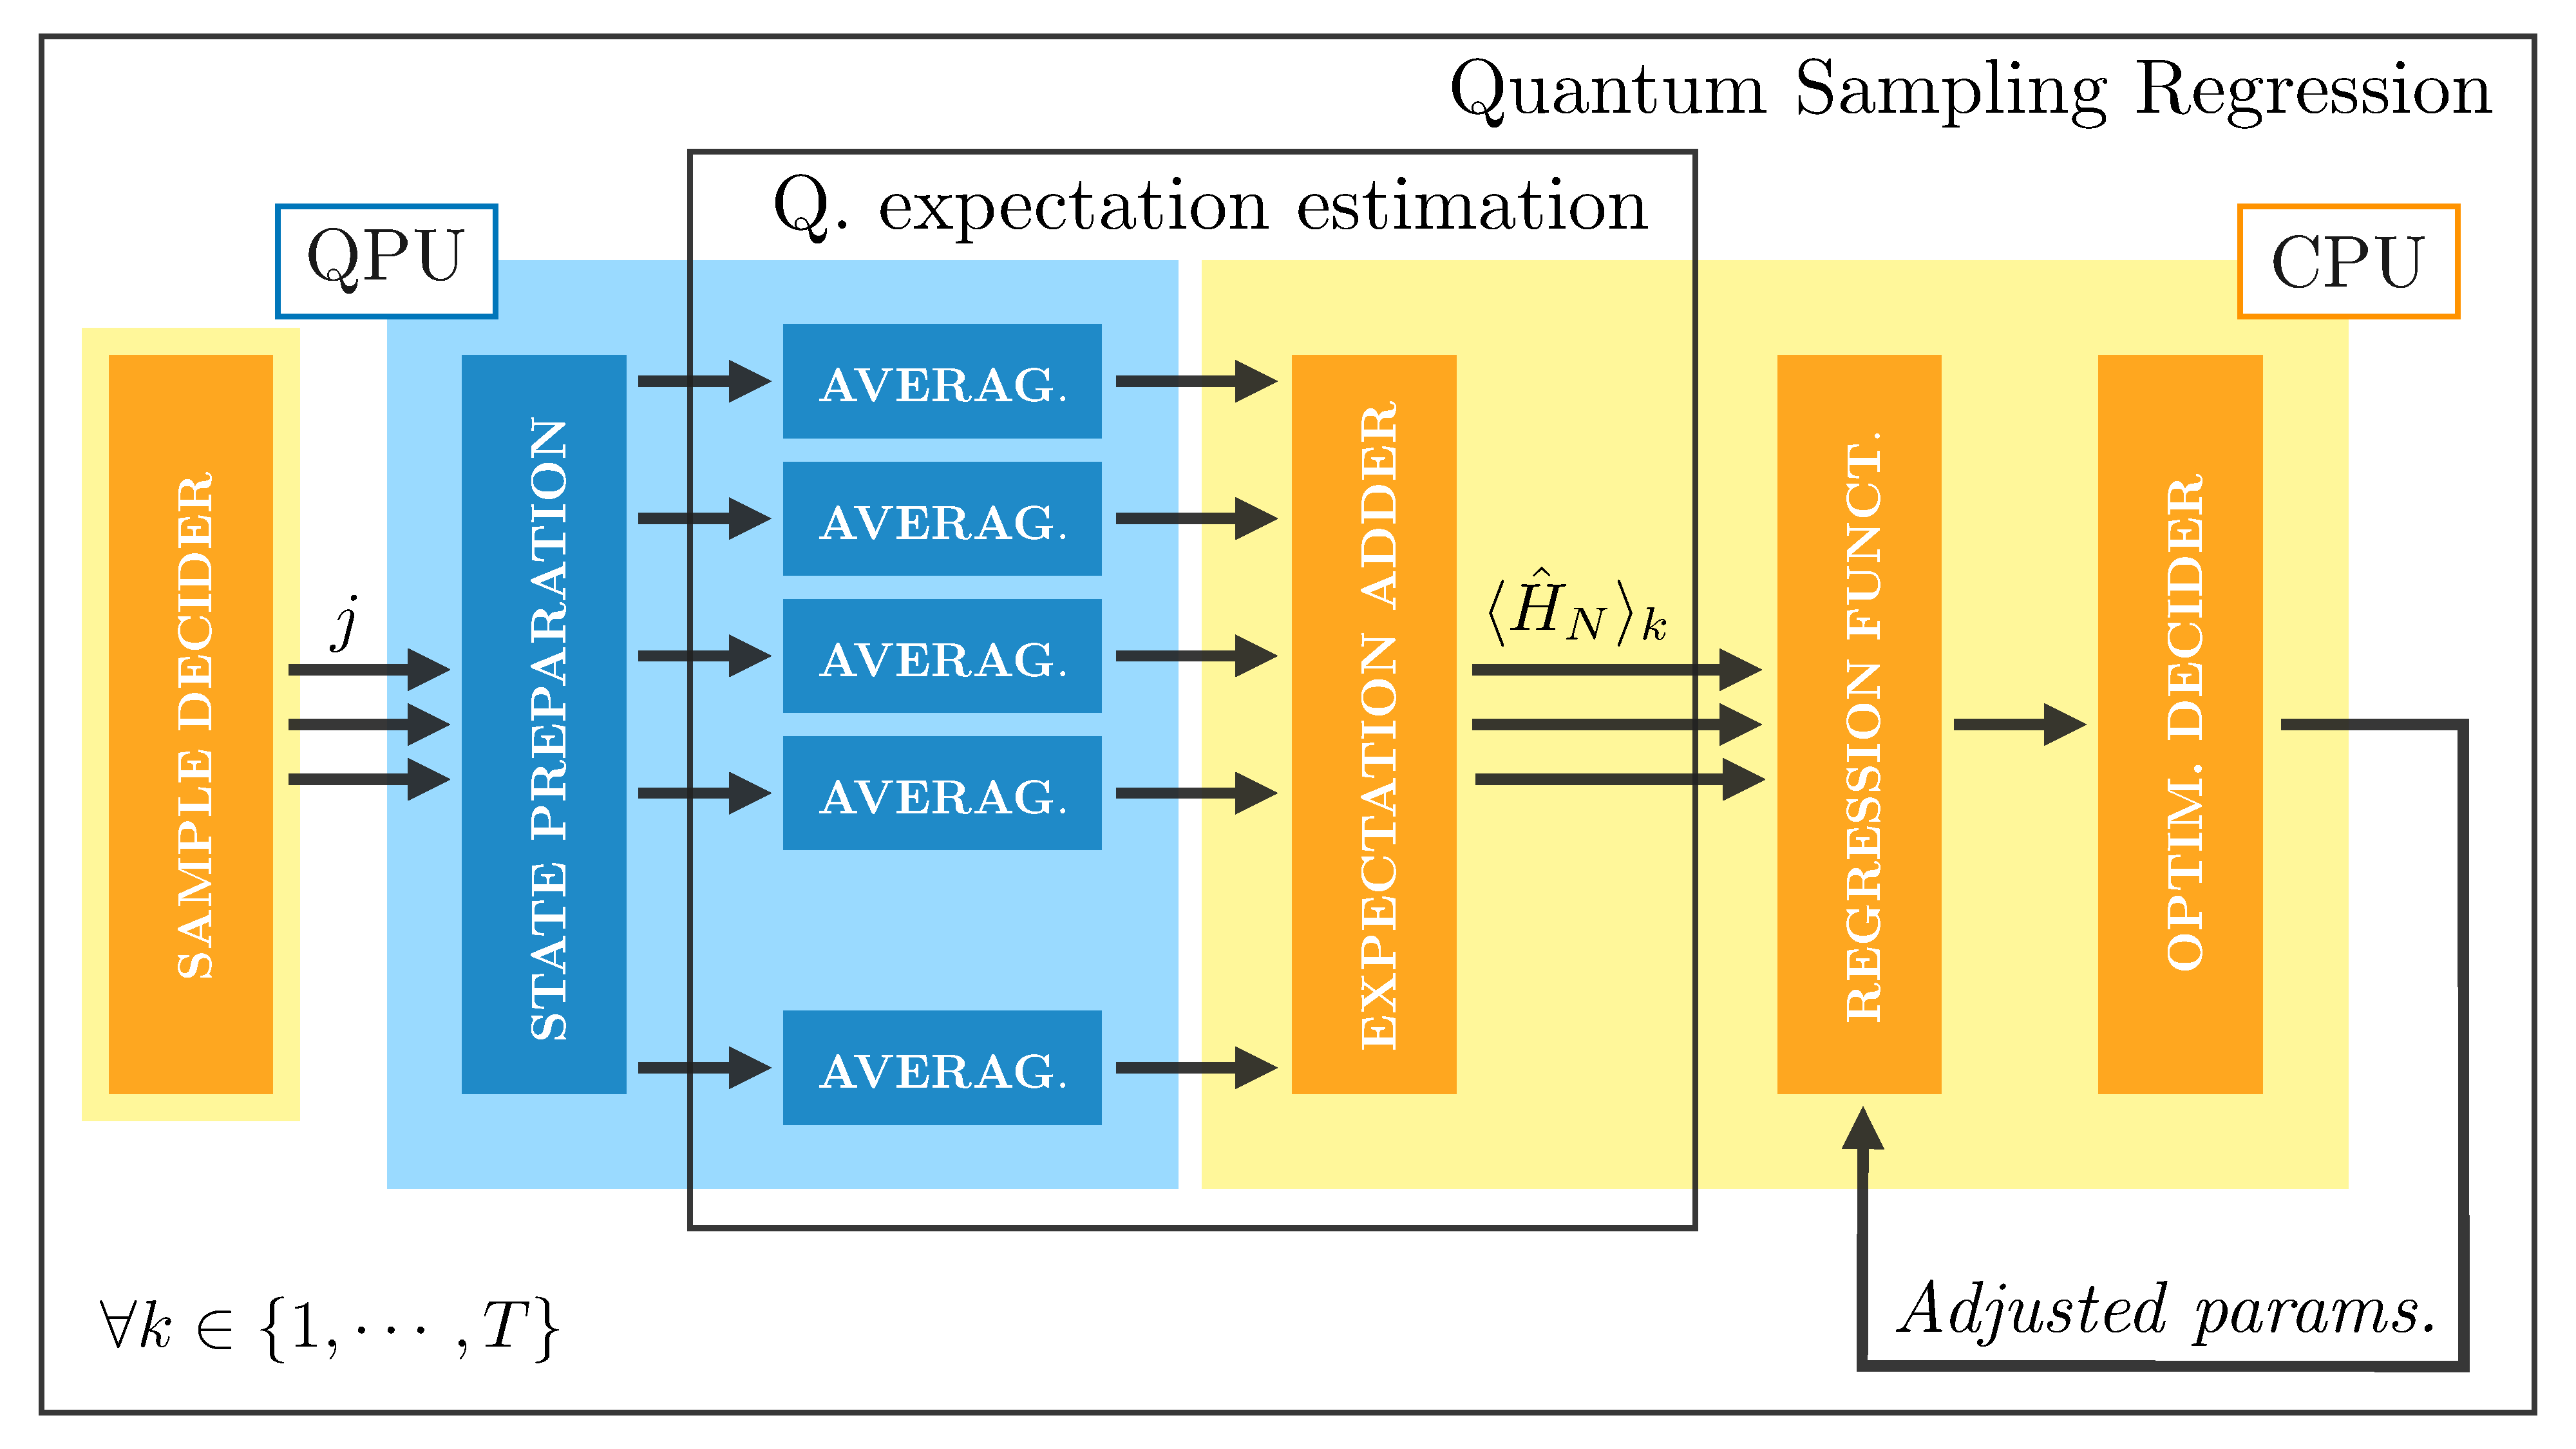
\includegraphics[width=.7\paperwidth]{Figures/chapter05/QSR}
    \end{center}
  \end{minipage}

%% ----------------------------------------------------------------------------
\break
%% ----------------------------------------------------------------------------

  \begin{multicols}{2}

    \begin{itemize}
      \item From the \textbf{topology of the quantum circuit} in charge of state preparation, we can infer a frequency bound.
      \item \textbf{Fourier analysis} then allows to fully reconstruct the expectation value function.
      \item Through the \textbf{Nyquist-Shannon sampling theorem} we can show that our sampling technique is optimal.
    \end{itemize}

    \columnbreak

    \begin{center}
      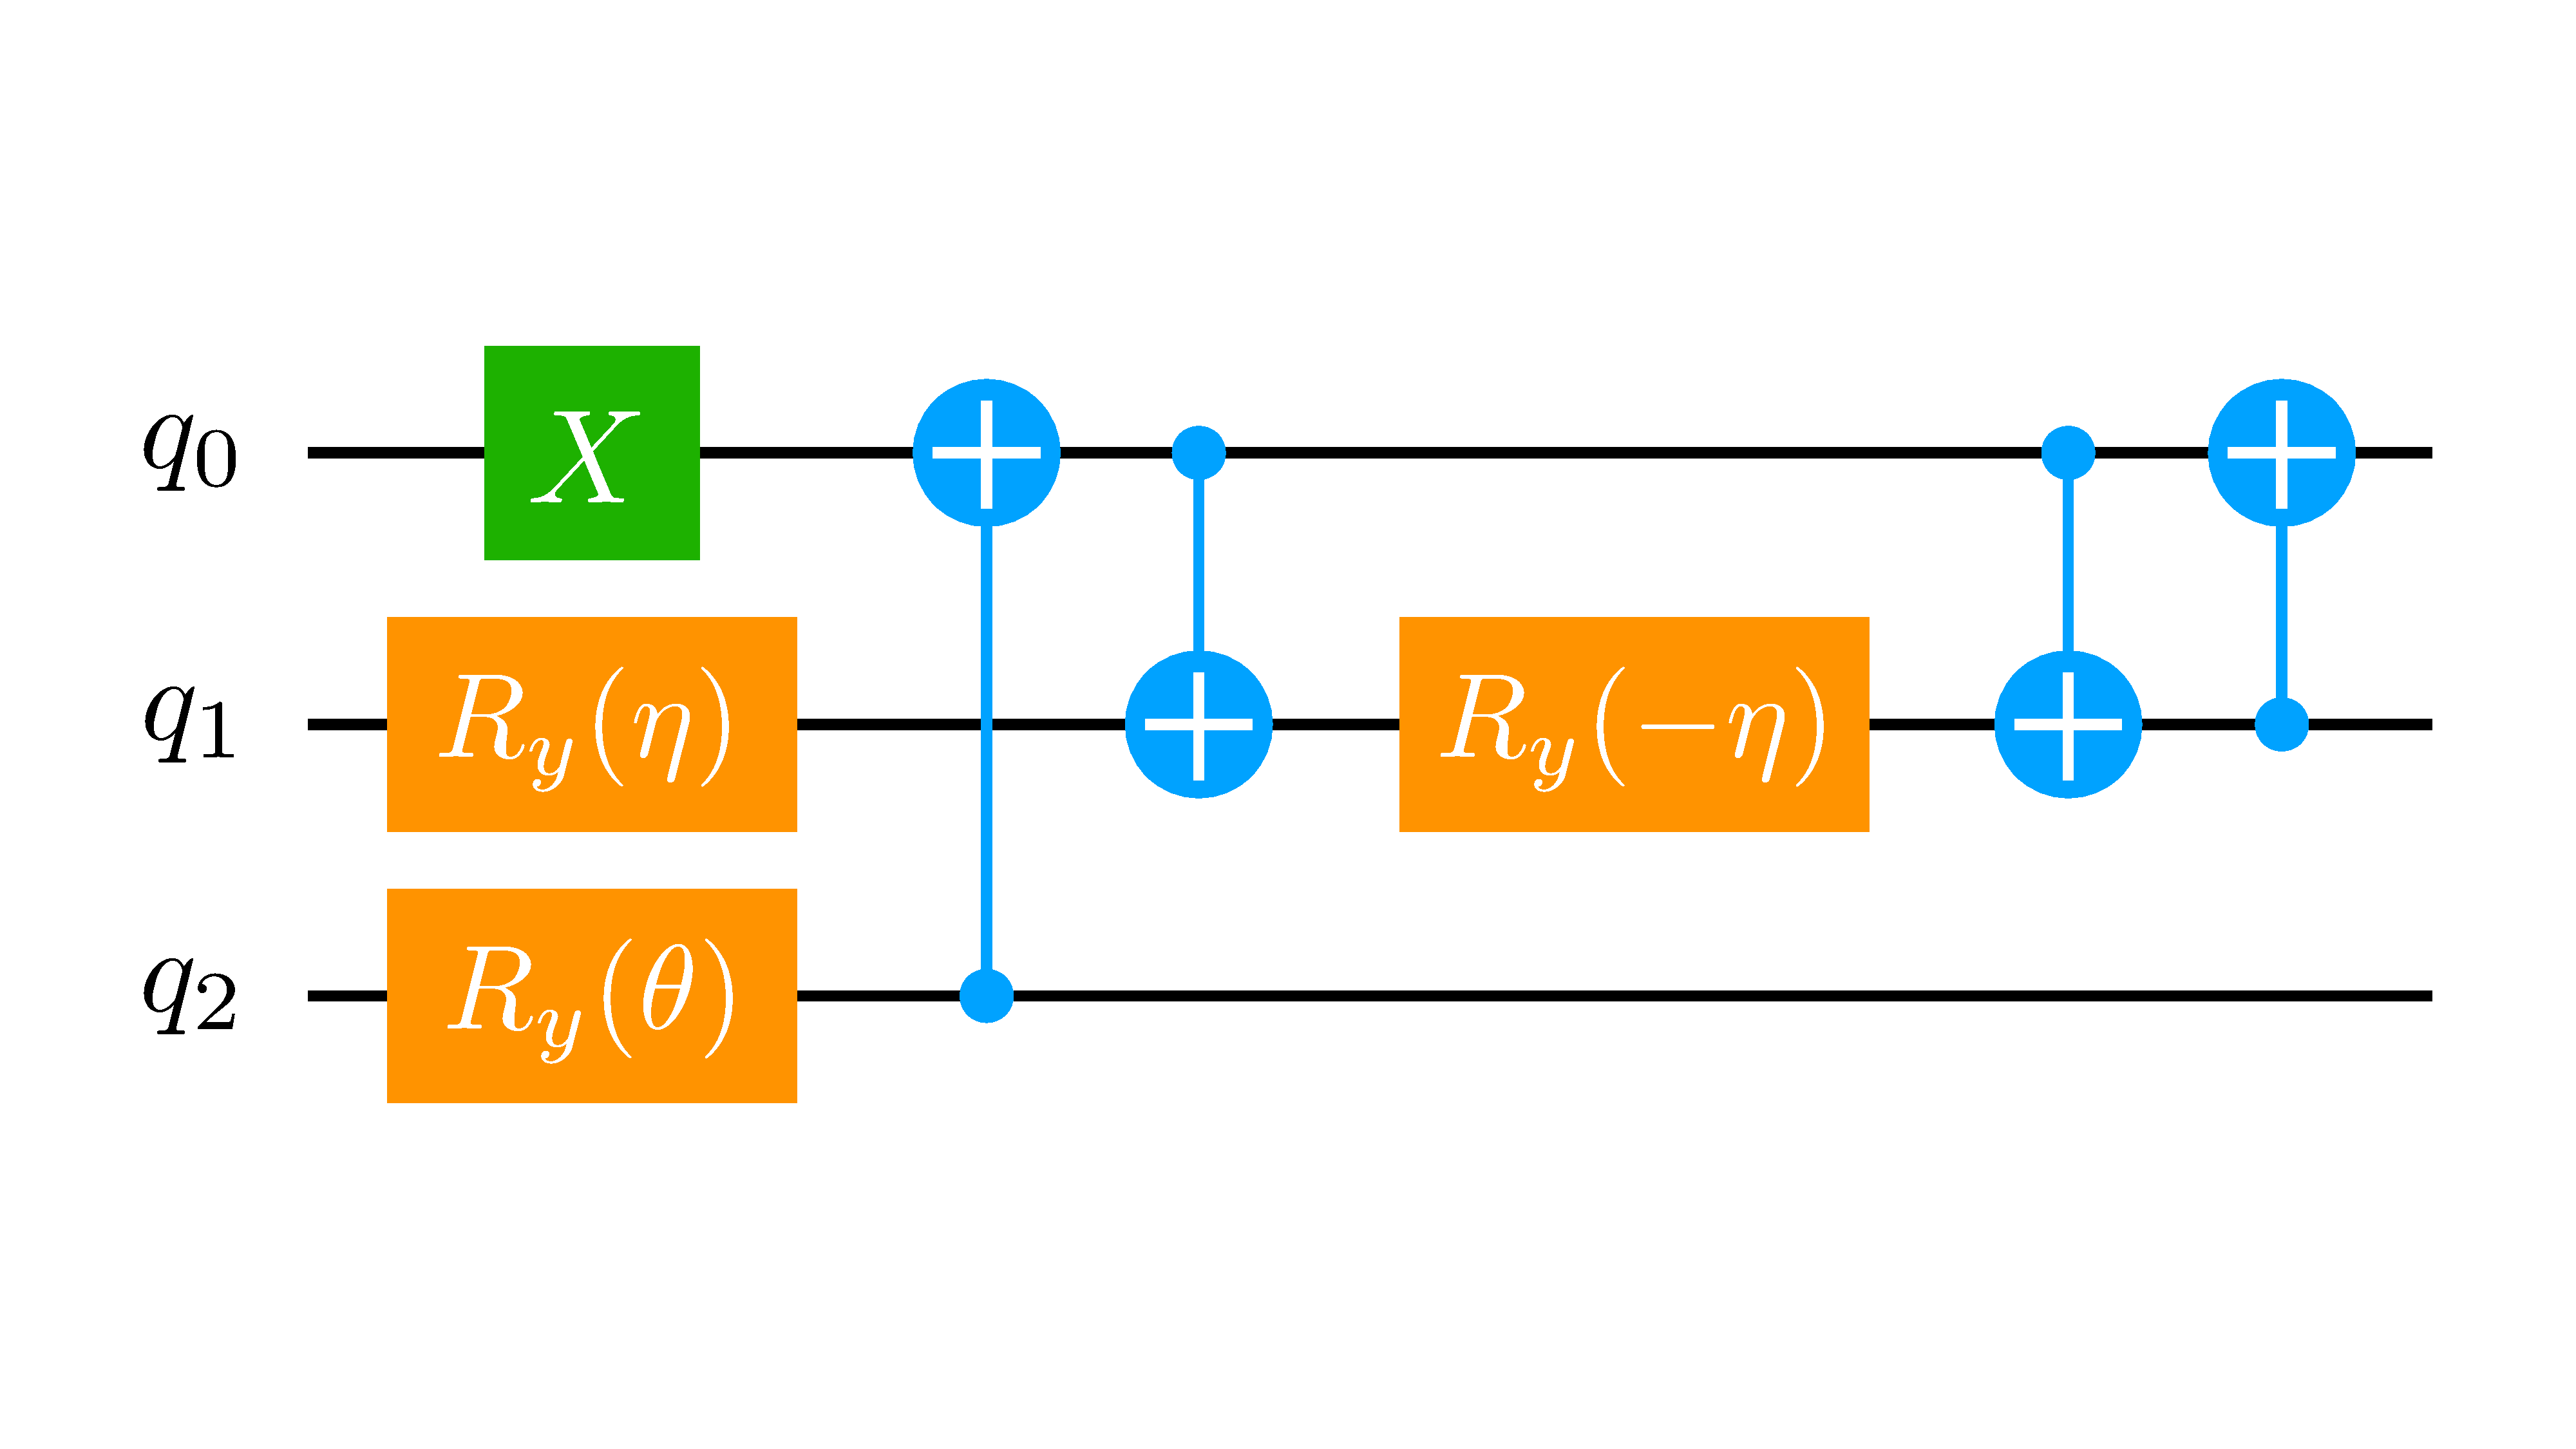
\includegraphics[width=.40\paperwidth]{Figures/chapter05/deuteron-quantum-circuits-2}
    \end{center}

  \end{multicols}

  \vspace{-1em}
  \begin{theorem}[Nyquist-Shannon]
    If a function $h(\theta)$ contains no angular frequencies higher than $\omega_{\textnormal{S}}$, it is completely determined by giving its ordinates at a series of points $1/2\omega_{\textnormal{S}}$ apart: $\omega_{\textnormal{sampling}} > 2\omega_{\textnormal{S}}$.
  \end{theorem}

\end{frame}

%% ----------------------------------------------------------------------------
%% ----------------------------------------------------------------------------

\subsection{Comparison}

\begin{frame}[allowframebreaks]{Algorithm comparison}

  \vspace{2em}
  \begin{itemize}
    \item Algorithmic complexity model:
  \end{itemize}
  \vspace{-2em}
  \begin{gather*}
    \frac{\textnormal{VQE}}{\textnormal{QSR}} = \qty(m n 2^{-n/r})^{p}
  \end{gather*}

  \vspace{-1em}
  \begin{multicols}{2}

    \begin{center}
      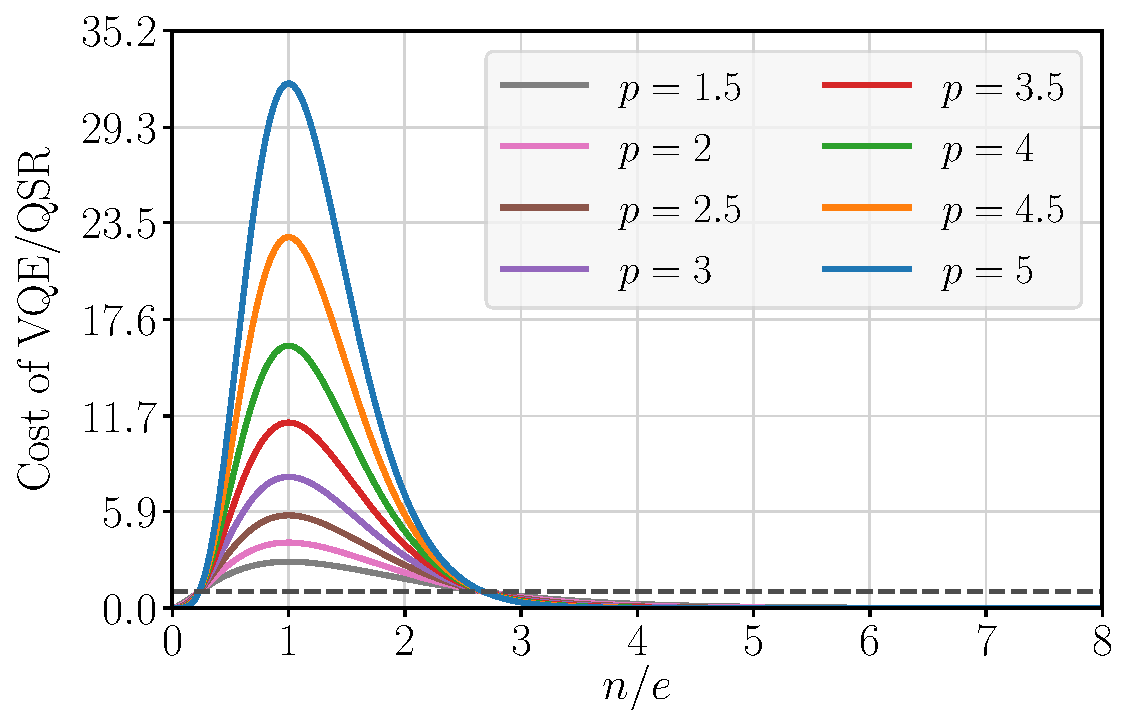
\includegraphics[width=.40\paperwidth]{Figures/chapter05/VQE-vs-QSR_p}
    \end{center}

    \columnbreak

    \begin{center}
      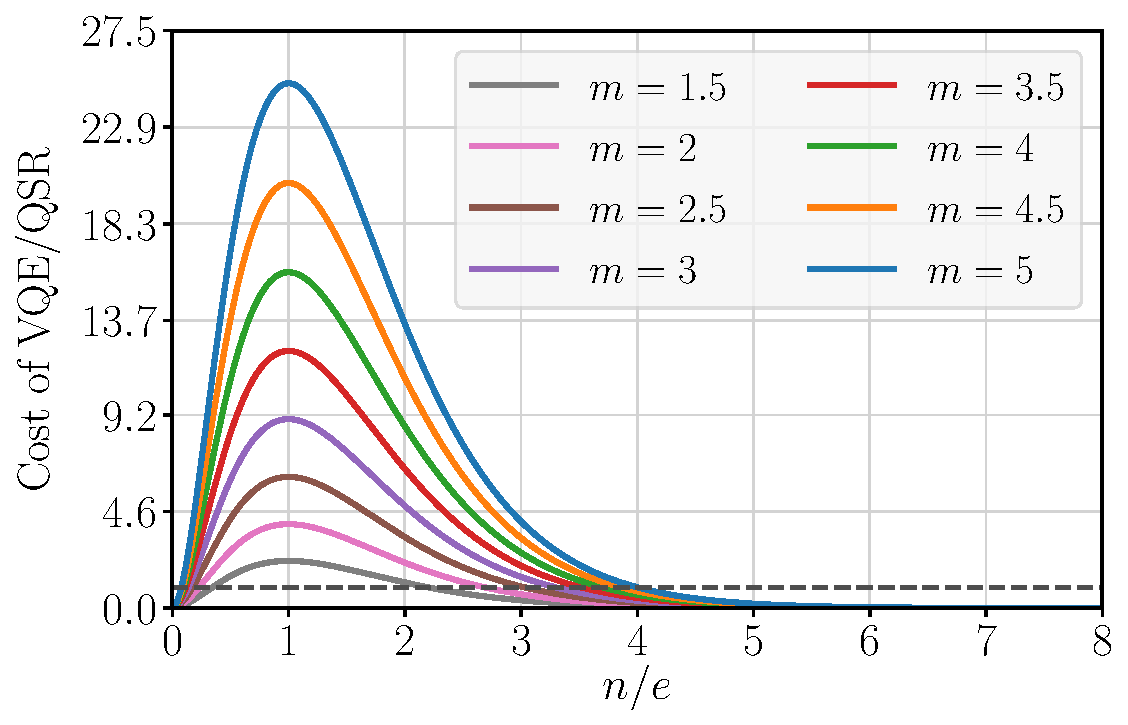
\includegraphics[width=.40\paperwidth]{Figures/chapter05/VQE-vs-QSR_m}
    \end{center}

  \end{multicols}

%% ----------------------------------------------------------------------------
\break
%% ----------------------------------------------------------------------------

  \begin{multicols}{2}

    \begin{center}
      Threshold \\
      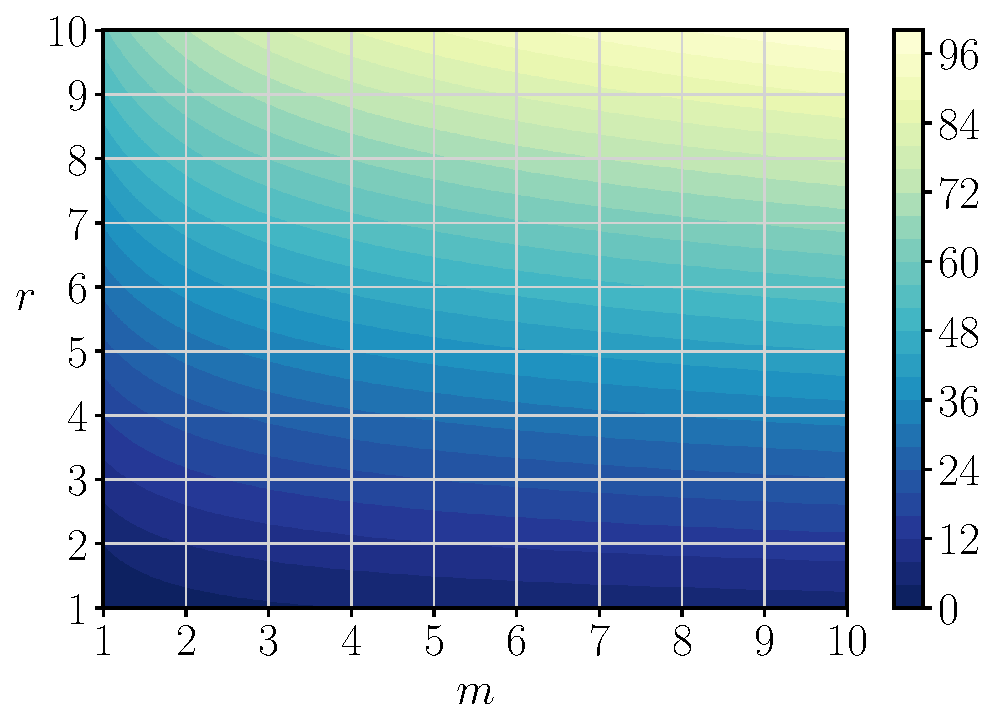
\includegraphics[width=.40\paperwidth]{Figures/chapter05/threshold}
    \end{center}

    \columnbreak

    \begin{center}
      Efficiency \\
      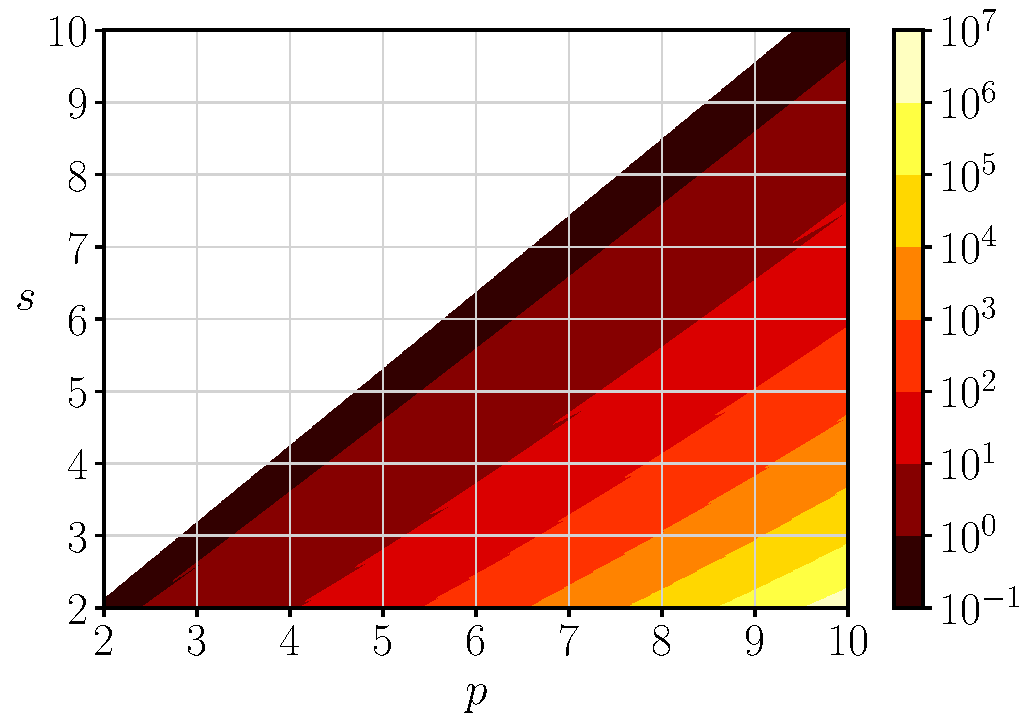
\includegraphics[width=.40\paperwidth]{Figures/chapter05/efficiency}
    \end{center}

  \end{multicols}
  \vspace{-3em}
  \begin{multicols}{2}

    \begin{gather*}
      a \defeq \ceil*{- \frac{r}{\ln{2}} W_{-1}\qty(-\frac{\ln{2}}{mr})}
    \end{gather*}

    \columnbreak

    \begin{gather*}
      E \approx \frac{1}{as\ln{2}} \qty(\frac{m}{s\ln{2}})^p
        \Gamma \qty(p+1, s\ln{2}, as\ln{2}) \label{eq:QSR-efficiency}
    \end{gather*}

  \end{multicols}

\end{frame}

%% ----------------------------------------------------------------------------
%% ----------------------------------------------------------------------------

\begin{frame}{Benchmark}

  \begin{figure}[!tbp]
  	\centering
  	\begin{minipage}[c]{.40\linewidth}
  		\centering
  		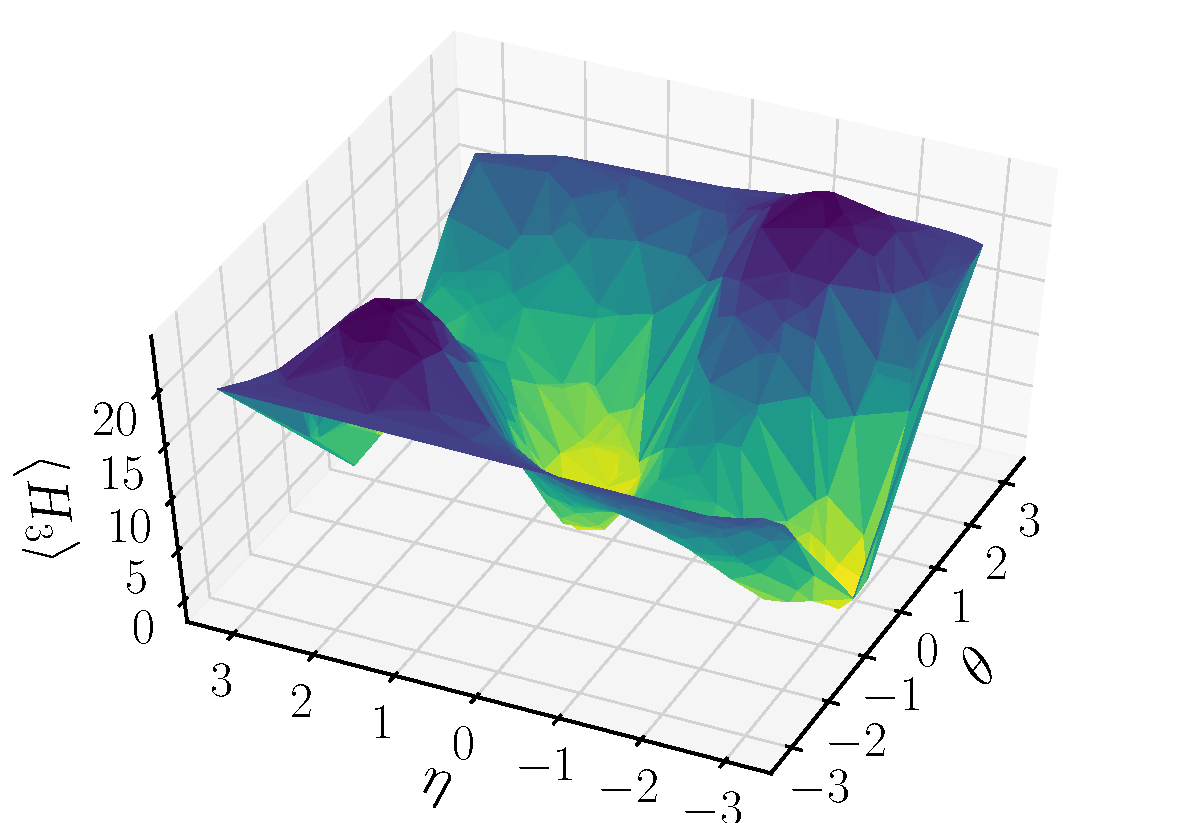
\includegraphics[width=\linewidth]{Figures/chapter05/deuteron-VQE}
  	\end{minipage}
  	\hspace{.025\linewidth}
  	\begin{minipage}[c]{.40\linewidth}
  		\centering
  		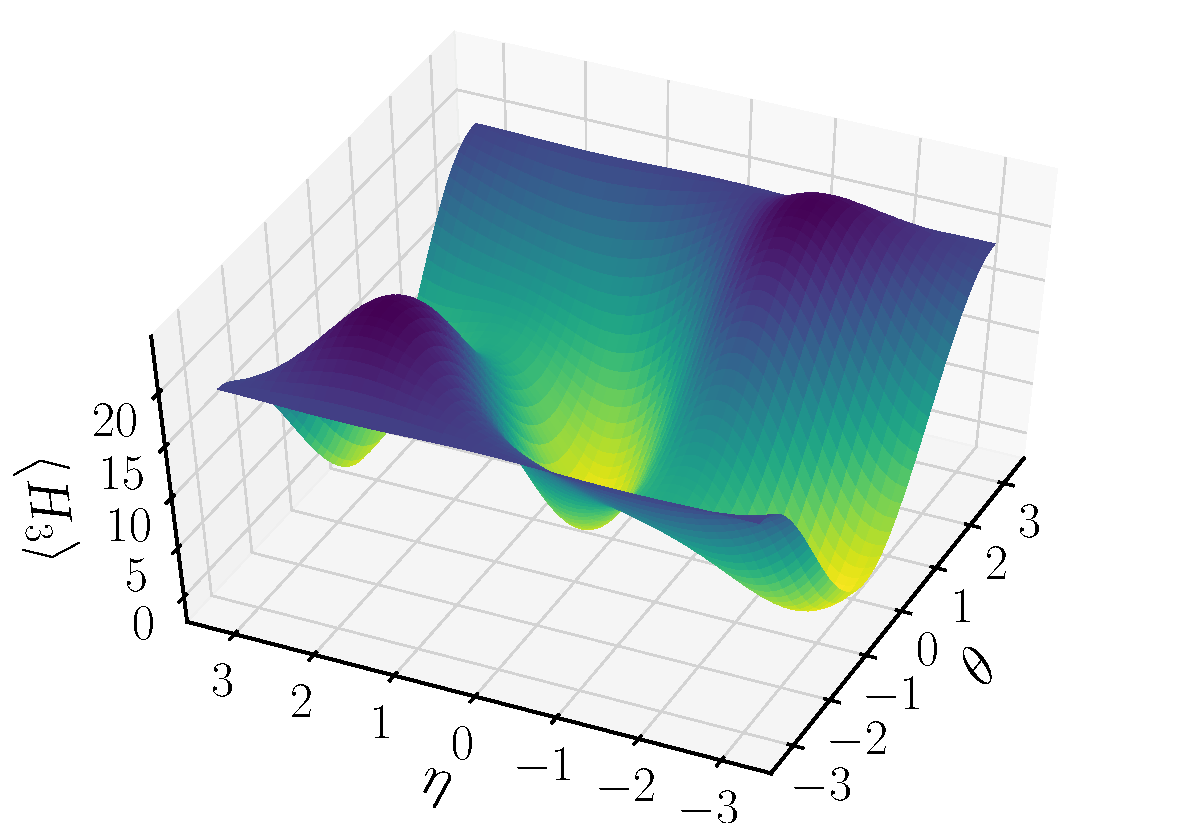
\includegraphics[width=\linewidth]{Figures/chapter05/deuteron-QSR}
  	\end{minipage}
  	\caption{Comparison between the VQE and QSR algorithms, when reproducing an external model with two parameters. (Left) Triangulation of the expectation value function from raw samples. (Right) Approximate function obtained through the Optimal Sampling Regression method with $S_q=S_{\text{max}}=2 ~\forall q$.}
  \end{figure}

  \vspace{-1em}

  \begin{table}[!bp]
  	\centering
  	% \caption{Comparison between results using the VQE and QSR algorithms.}
  	\begin{tabular}{ c c c c c }
  		\hline
  		\hline
  		$N_\text{params}$ & VQE samples & QSR samples &
  		VQE error & QSR error \\
  		\hline
  		$1$ & $24$ & $3$ & $3.5\%$ & $1.0\%$ \\
  		$2$ & $153$ & $25$ & $0.3\%$ & $0.2\%$ \\
  		\hline
  		\hline
  	\end{tabular}
  \end{table}

\end{frame}

%% ----------------------------------------------------------------------------
%% ----------------------------------------------------------------------------

\subsection{Applications}

%% ----------------------------------------------------------------------------
%% ----------------------------------------------------------------------------

\begin{frame}{Applications of QSR}

  \begin{multicols}{2}
    \begin{itemize}
      % \item \textbf{Reduce the amount of queries} necessary to solve a given optimization problem.
      \item \textbf{Oversampling} to attain higher precision.
      \item \textbf{Undersampling} to boost performance and get rid of small-wavelength oscillations leading to burdensome local minima.
      \item VQE low-resolution start-up \textbf{supplement}.
      \item \textbf{Proxy} to transition between simulators and real devices.
      \item Improve convergence by removing the stochastic nature of the quantum expectation value function.
      \item Avoid the exponential matrix formulation in classical computation.
    \end{itemize}

    \columnbreak

    \begin{center}
      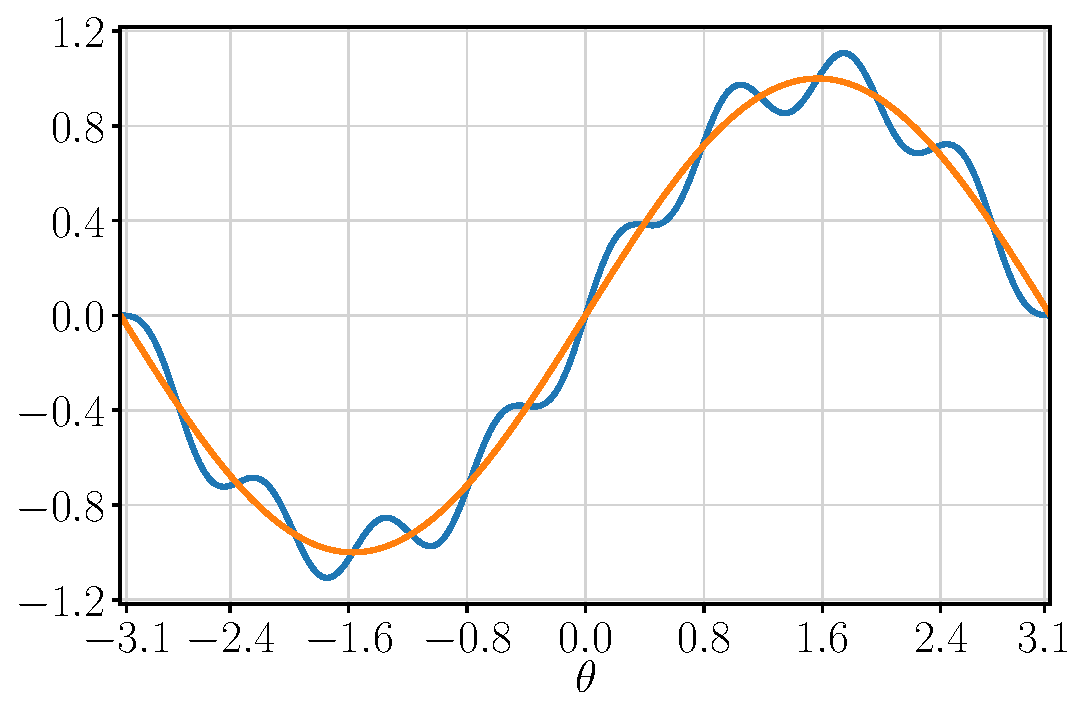
\includegraphics[width=.40\paperwidth]{Figures/low-resolution}
    \end{center}

  \end{multicols}

\end{frame}

%%    _____  _____
%%   |  __ \|  __ \    AUTHOR: Pedro Rivero
%%   | |__) | |__) |   ---------------------------------
%%   |  ___/|  _  /    DATE: November 10, 2021
%%   | |    | | \ \    ---------------------------------
%%   |_|    |_|  \_\   https://github.com/pedrorrivero
%%

\section{Conclusions and future research}

%% ----------------------------------------------------------------------------
%% ----------------------------------------------------------------------------

\begin{frame}{Conlcusions}

	\begin{itemize}
		\item I showcased an instance of hadron mass generation in QCD using the NJL model in $1+1$ dimensions and $2$ flavors.
    \item I discovered a clear transition from a regime dominated by the quark masses, to a regime dominated by their interaction.
    \item I compiled and developed the computational techniques necessary for efficiently simulating Quantum Field Theories on a quantum computer.
    \item I established how revealing these kind of problems can be when addressed on quantum computers, and why Quantum Field Theory should remain a key motivation for developing QIS methods and techniques.
	\end{itemize}

\end{frame}

%% ----------------------------------------------------------------------------

\begin{frame}{Future research}

  \begin{itemize}
    \item Calculation of parton distribution functions and form factors for the study of Deep inelastic scattering.
    \item Repeat calculations with other mappings and parametrization ansatzes.
    \item Increase the dimensions of our problem to $2+1$, and $3+1$.
    \item Explore other quantum field theories up to full QCD.
    \item Formalize the scalabilty of these techniques in the NISQ era and beyond.
    \item Develop a robust notation for these applications of QIS.
  \end{itemize}

\end{frame}



%% ----------------------------------------------------------------------------
%% BACK-MATTER
%% ----------------------------------------------------------------------------

% \section{Bibliography}
% %	\begin{frame}[allowframebreaks]{Bibliography}
% \begin{frame}{Bibliography}
%
% 	\begin{thebibliography}{9}
% 		\setbeamertemplate{bibliography item}[online]
% 	\bibitem{hayden} \textbf{Hayden, P.} \emph{Quantum Computational Universe}
% 		\setbeamertemplate{bibliography item}[book]
% 	\bibitem{susskind_book} \textbf{Susskind, L. \& Friedman A.} \emph{Quantum Mechanics: The Theoretical Minimum}
% 		\setbeamertemplate{bibliography item}[book]
% 	\bibitem{nielsen} \textbf{Nielsen M.A. \& Chuang I.L.} \emph{Quantum Computation and Quantum Information}
% 		\setbeamertemplate{bibliography item}[article]
% 	\bibitem{ladd} \textbf{Lykken J.} \emph{Quantum Technologies for Quantum Science}
% 		\setbeamertemplate{bibliography item}[book]
% 	\bibitem{mermin} \textbf{Mermin N.D.} \emph{Quantum Computer Science: An Introduction}
% 		\setbeamertemplate{bibliography item}[article]
% 	\bibitem{ladd} \textbf{Ladd T.D. (et al.)} \emph{Quantum Computing}
%
% 	\end{thebibliography}
%
% 	\vspace{20pt}
% 	\begin{small}
% 	\begin{center}{
% 	\color{gray}
% 		\emph{"The only thing demonstrated by an impossibility proof is a lack of imagination."} \\
% 		\textbf{– John Stewart Bell –} }
% 	\end{center}
% 	\end{small}
% \end{frame}

%% ----------------------------------------------------------------------------

\FinalFrame


%% ----------------------------------------------------------------------------
%% EXTRA SLIDES
%% ----------------------------------------------------------------------------

% %%    _____  _____
%%   |  __ \|  __ \    AUTHOR: Pedro Rivero
%%   | |__) | |__) |   ---------------------------------
%%   |  ___/|  _  /    DATE: November 10, 2021
%%   | |    | | \ \    ---------------------------------
%%   |_|    |_|  \_\   https://github.com/pedrorrivero
%%

\begin{frame}[allowframebreaks]{Quantum Fourier transform}

	The usual \textbf{Discrete Fourier Transform} (DFT) can be expressed as:

	\medskip

	\begin{align*}
	  \ket{j} \qra&
				\frac{1}{\sqrt{N}} \sum_{k=0}^{N-1} \exp[2\pi i \frac{jk}{N}] \ket{k} \\
	    =& \frac{1}{2^{n/2}} \sum_{k_{n-1}=0}^{1} \cdots \sum_{k_{0}=0}^{1}
	      \exp[2\pi ij \qty(\sum_{l=0}^{n-1} k_{l} 2^{l-n})]
	      \ket{\bin k_{n-1} \dots k_{0}} \\
	    =& \frac{1}{2^{n/2}} \sum_{k_{n-1}=0}^{1} \cdots \sum_{k_{0}=0}^{1}
	      \qty{ \bigotimes_{l=1}^{n} \exp[2\pi ij k_{n-l} 2^{-l}]
	      \ket{k_{n-l}} } \\
	    =& \frac{1}{2^{n/2}} \bigotimes_{l=1}^{n}
	      \qty{ \sum_{k_{n-l}=0}^{1} \exp[2\pi ij k_{n-l} 2^{-l}] \ket{k_{n-l}} }
	    = \frac{1}{2^{n/2}} \bigotimes_{l=1}^{n}
	      \qty{ \ket{0} + \exp[2\pi ij 2^{-l}] \ket{1} }
	\end{align*}

\break

	\begin{gather*}
		\ket{j} \ra
			\frac{
				\qty{\ket{0}+ e^{2\pi i \qty(\bin.j_{0})} \ket{1}} \otimes
				\qty{\ket{0}+ e^{2\pi i \qty(\bin.j_{1}j_{0})} \ket{1}} \otimes
				\cdots \otimes
				\qty{\ket{0} + e^{2\pi i \qty(\bin.j_{n-1}j_{n-2} \dots j_{0})} \ket{1}}
			}{2^{n/2}} \\[10pt]
		R_{k} \defeq \mqty[1 & 0 \\ 0 & e^{2\pi i/2^k}]
	\end{gather*}

	\vspace{-2em}

	\begin{center}
		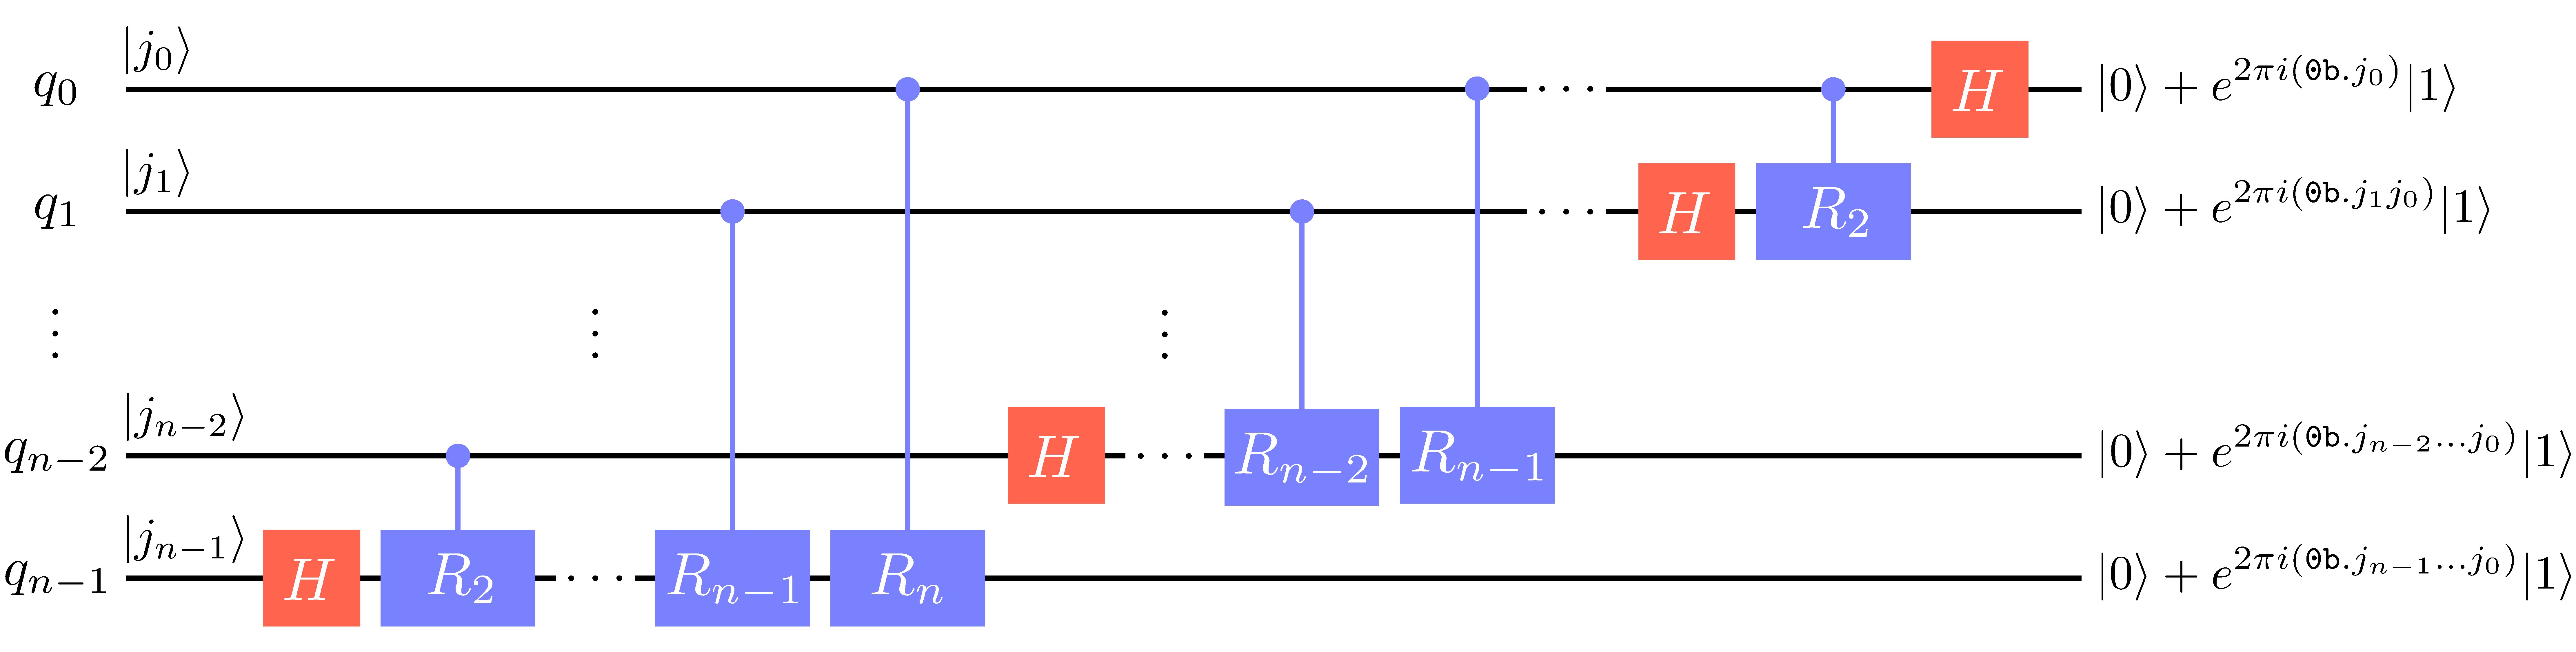
\includegraphics[width=.80\paperwidth]{Figures/quantum-background/quantum-fourier-transform}
	\end{center}

\break

	We can now compare the complexity of this algorithm with its best classical counterparts. This is done by counting the number of gates in the circuit, where we have to remember the final SWAP gates omitted in the representation.

	\begin{multicols}{2}
	\begin{centering}

		\underline{\textbf{FAST FOURIER TRANSFORM}}\\
		\medskip
		$N\log_2 N \equiv \Theta\qty(n2^n)$

		\columnbreak

		\underline{\textbf{QUANTUM FOURIER TRANSFORM}}\\
		\medskip
		$\sum_{k=1}^{n}k + \frac{n}{2} =
			\frac{n\qty(n+1)}{2} + \frac{n}{2} \equiv \Theta\qty(n^2)$

	\end{centering}
	\end{multicols}

	Nonetheless, this technique cannot be used directly for computing the target transform; since we do not know how to recover the individual amplitudes from the quantum states. On top of that, there is no efficient general method for preapring the states to be transformed. This is a great example of an algorithm that presents huge savings compared to its classical analogs, but which cannot be generally used as much as we would like to due to our inability to extract the desirerd information. In some instances however, we can profit from this method to great deeds ---mainly as part of bigger algorithms. An important application is \textbf{Shor's factoring algorithm}, which can be used for efficiently finding the prime decomposition of any given number.

\end{frame}

% %%    _____  _____
%%   |  __ \|  __ \    AUTHOR: Pedro Rivero
%%   | |__) | |__) |   ---------------------------------
%%   |  ___/|  _  /    DATE: November 10, 2021
%%   | |    | | \ \    ---------------------------------
%%   |_|    |_|  \_\   https://github.com/pedrorrivero
%%

\begin{frame}[allowframebreaks]{Unitary coupled cluster}

	The motivation behind coupled cluster methods arises from the idea of explorinig only the regions of phase space close to an initial \textbf{reference state}. The choice of said reference state is of great importance for retreiving successful results. Let us begin by choosing the region of study in terms of \textbf{Hamming distance} (i.e. bit flips). This is sometimes called \textbf{configuration interaction} (CI). Using a notation where $\sigma^{p}_{n} \equiv \sigma^{p}(n)$ we can write any state one spin flip away from the initial reference state as:

	\begin{gather*}
	  \ket{\text{CI}_{1} \qty(z^{n})} \defeq
	    \sum_{n} z^{n} \sigma^{+}_{n} \ket{\text{SR}}
	\end{gather*}

	\vspace{-1em}

	This approach can be easily extended to account for more and more states:

	\begin{gather*}
	  \ket{\text{CI}_{k} \qty(\boldsymbol{z})} \defeq
	    \sum_{j=1}^{k} T_{j} \qty(z^{n_1,\cdots,n_j}) \ket{\text{SR}} \\
	  T_{j} \qty(z^{n_1,\cdots,n_j}) \defeq \sum_{n_1,\cdots,n_j}
	    z^{n_1,\cdots,n_j} \sigma^{+}_{n_1} \! \cdots \sigma^{+}_{n_j}
	\end{gather*}

\break

	However, this approach presents a number of deficiencies which render it non-optimal; the biggest one for us being that it presents no clear advatadge over classical state preparation. The idea behind \textbf{coupled cluster} (CC) consists on using the spin flips as generators instead:

	\begin{gather*}
	  \ket{\text{CC}_{k} \qty(\boldsymbol{z})} \defeq
	    \exp[\sum_{j=1}^{k} T_{j} \qty(z^{n_1,\cdots,n_j})]
	    \ket{\text{SR}}
	\end{gather*}

	In order to make this ansatz suitable for quantum processors, we need to express it in terms of unitary transformations. We have finally arrived at \textbf{unitary coupled cluster} (UCC):

	\begin{gather*}
	  \ket{\text{UCC}_{k} \qty(\boldsymbol{\theta},\boldsymbol{\eta})} \defeq
	    \exp[
	      \sum_{j=1}^{k} T_{j}^{-} \qty(\theta^{n_1,\cdots,n_j}) + i
	      \sum_{j=1}^{k} T_{j}^{+} \qty(\eta^{n_1,\cdots,n_j})
	    ]
	    \ket{\text{SR}} \\
	    T_{j}^{\pm} \qty(\theta^{n_1,\cdots,n_j}) \defeq
	      \sum_{n_1,\cdots,n_j} \theta^{n_1,\cdots,n_j} \qty(
	        \sigma^{+}_{n_1} \! \cdots \sigma^{+}_{n_j} \: \pm \:
	        \sigma^{-}_{n_1} \! \cdots \sigma^{-}_{n_j}
	      )
	\end{gather*}

\break

	Another important version of this ansatz is developed in a \textbf{fermionic basis} (i.e. for parametrizing Fock space instead of Hilbert space), and replaces spin-flips with changes in the state of particles. This is interesting because, due to the non-locality of the Jordan-Wigner transform, if we were to apply the unitary coupled cluster parametrization directly onto the Jorda-Wigner's mapping image (i.e. Hilbert space), we might be exploring uninteresting regions of the domain (i.e. Fock space) ---such as those containing symmetry-broken states. On top of that, this method is usually developed so that it \textbf{conserves the total number of particles} in the system; which is predefined through the fermion reference (FR):

	\begin{gather*}
	  \ket{\text{FUCC}_{k} \qty(\boldsymbol{\theta},\boldsymbol{\eta})} \defeq
	    \exp[
	      \sum_{j=1}^{k} F_{j}^{-} \qty(\theta^{p_1,\cdots,p_j,q_1\cdots,q_j}) +i
	      \sum_{j=1}^{k} F_{j}^{+} \qty(\eta^{p_1,\cdots,p_j,q_1\cdots,q_j})
	    ]
	    \ketf{\text{FR}}_{\mathcal{Q}} \\
	    F_{j}^{\pm} \qty(\theta^{p_1,\cdots,p_j,q_1\cdots,q_j}) \defeq
	      \sum_{\substack{q \in \mathcal{Q} \\ p \in \overline{\mathcal{Q}}}}
	      \theta^{p_1,\cdots,p_j,q_1\cdots,q_j} \qty(
	        \phi^{\dagger}_{p_1} \! \cdots \phi^{\dagger}_{p_j} \,
	        \phi_{q_1} \! \cdots \phi_{q_j} \: \pm \:
	        \phi^{\dagger}_{q_1} \! \cdots \phi^{\dagger}_{q_j} \,
	        \phi_{p_1} \! \cdots \phi_{p_j}
	      )
	\end{gather*}

\end{frame}

% %%    _____  _____
%%   |  __ \|  __ \    AUTHOR: Pedro Rivero
%%   | |__) | |__) |   ---------------------------------
%%   |  ___/|  _  /    DATE: November 10, 2021
%%   | |    | | \ \    ---------------------------------
%%   |_|    |_|  \_\   https://github.com/pedrorrivero
%%

\section{State preparation}

%% ----------------------------------------------------------------------------

\begin{frame}{Space parametrization and state preparation}

	Once we have ways of measuring our Hamiltonian, we need to be able to explore different quantum states; a process known as \textbf{state preparation}. This can be achieved by parametrizing the Hilbert/Fock space of states representing the system, and finding a way to prepare the corresponding quantum state in the processor given any combination of those parameters.

	\begin{multicols}{2}

		For this task we will be employing some of the IBM-Q quantum computers and simulators; accessible through the cloud via the \texttt{Qiskit} framework. Nevertheless, there is one major shortcoming: the dimension of the space at hand grows exponentially with the number of qubits $2N$ used in the representation of the system. This means that the parametrization will become too large to handle both in state of the art and forthcoming machines unless it is treated in a smart way.

		\columnbreak

		\begin{center}
			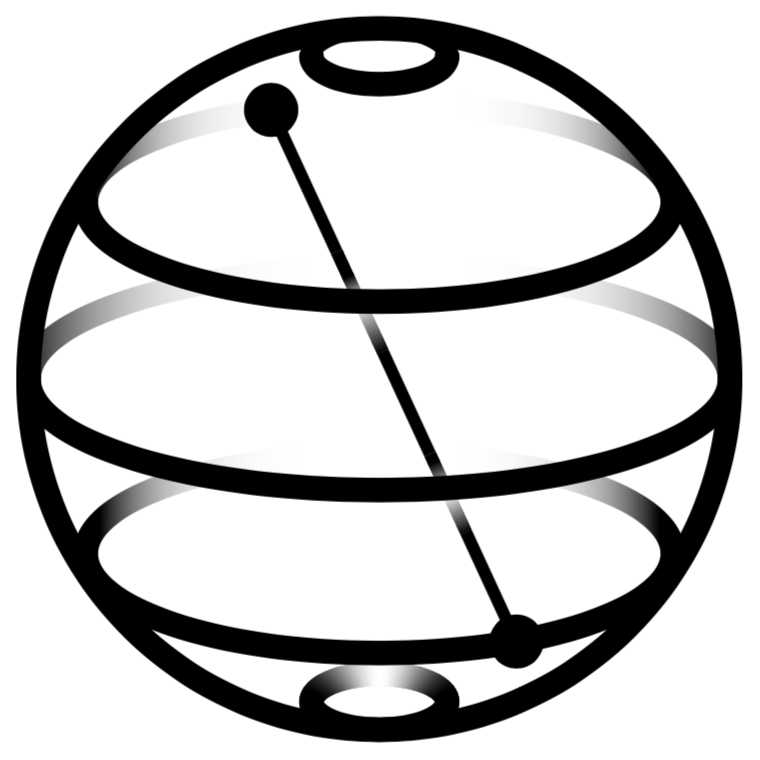
\includegraphics[width=.2\paperwidth]{Figures/qiskit}
		\end{center}
		\begin{center}
			
\includegraphics[width=.1\paperwidth]{Figures/ibm}
		\end{center}

	\end{multicols}

\end{frame}

%% ----------------------------------------------------------------------------

\begin{frame}[allowframebreaks]{Custom symmetry-based parametrization ansatz}

	While general, it is easy to notice that the implementation of any variant of the unitary coupled cluster ansatz is still cumbersome and can depend on a large number of parameters based on the chosen order of truncation. We will now introduce a new ansatz inspired by the shape of our refactored Hamiltonian. For this task, we will analyze the two distinct parts in our Hamiltonian independently; since these will dominate in two \textbf{different regimes}:

	\begin{multicols}{2}

		\begin{center}
			\underline{\textbf{INFINITELY STRONG INTERACTIONS}}\\
			\small{\emph{Interaction term dominates (i.e. $G_{\pi} \ra \infty$)}}
			\begin{gather*}
				G_{N} \defeq \sum_{n=0}^{N-1} Z_{2n+1}Z_{2n}
			\end{gather*}
		\end{center}

		\columnbreak

		\begin{center}
			\underline{\textbf{INFINITELY WEAK INTERACTIONS}}\\
			\small{\emph{Kinetic term dominates (i.e. $G_{\pi} \ra 0$)}}
			\begin{gather*}
			  K_{N} \defeq \sum_{n=0}^{2N-1} \qty[ X_{n+1}Y_{n} - Y_{n+1}X_{n} ]
			\end{gather*}
		\end{center}

	\end{multicols}

	Let us call each computational basis state by the decimal translation of its binary form:

	\begin{gather*}
	  \ket{0} \defeq \ket{\bin\dots0000} \qc
	  \ket{1} \defeq \ket{\bin\dots0001} \qc
	  \ket{2} \defeq \ket{\bin\dots0010} \qc
	  \cdots
	\end{gather*}

%% ----------------------------------------------------------------------------
\break
%% ----------------------------------------------------------------------------

	For the \textbf{interaction term} we notice that:

	\medskip

	\begin{itemize}
	  \item We can cycle in steps of two computational lattice sites.
	  \item We can change the position of any theoretical lattice site; since the interaction only occurs between positive and negative energy components at the same spot.
	  \item We can interchange positive and negative components in any number of theoretical lattice sites. We call each of these a \emph{swap transformation}.
	  \item We can flip every component $0 \lra 1$ in any number of theoretical lattice sites. We call each of these a \emph{flip transformation}.
	\end{itemize}

	\medskip

	This means that for $N=2$ (i.e. $2^{2N}=16$ basis states):

	\begin{gather*}
	  \ket{0} \equiv \ket{3} \equiv \ket{12} \equiv \ket{15} \\
	  \ket{1} \equiv \ket{2} \equiv \ket{4} \equiv \ket{7} \equiv
	    \ket{8} \equiv \ket{11} \equiv \ket{13} \equiv \ket{14} \\
	  \ket{5} \equiv \ket{6} \equiv \ket{9} \equiv \ket{10}
	\end{gather*}

%% ----------------------------------------------------------------------------
\break
%% ----------------------------------------------------------------------------

	Which represent the partition in degenerate subspaces of associated eigenvalues $\qty{+2,0,-2}$ respectively. These eigenvalues come from each theoretical lattice site in the spin-Z basis contributing with either $\pm 1$. Notice that the eigenvalues of this operator are always symmetrically disposed about zero, which means that $\forall N$:

	\begin{gather*}
	  \gamma_{\text{max}}^{N} = - \gamma_{\text{min}}^{N}
	\end{gather*}

	The interaction is maximum inside any theoretical lattice site whenever there is equal presence of both positive and negative energy components; conversely, the interaction is minimum whenever there is only one component present. Of course, the maximum (minimum) of the operator occurs when all theoretical lattice sites are maximized (minimized) individually:

	\begin{gather*}
	  \ket{\gamma_{\text{max}}}_{n} \in \{\ket{\bin00}, \ket{\bin11}\} \qc
	  \ket{\gamma_{\text{min}}}_{n} \in \{\ket{\bin01}, \ket{\bin10}\} \\[5pt]
	  \ket{\gamma_{\text{max}}^{N}} \equiv
	    \ket{\gamma_{\text{max}}}^{\otimes N} \qc
	  \ket{\gamma_{\text{min}}^{N}} \equiv
	    \ket{\gamma_{\text{min}}}^{\otimes N}
	\end{gather*}

%% ----------------------------------------------------------------------------
\break
%% ----------------------------------------------------------------------------

	Moving on to the \textbf{kinetic term} we have:

	\medskip

	\begin{itemize}
	  \item We can cycle in steps of one computational lattice site. We call this a \emph{cycling transformation}.
	  \item We cannot change the position of any theoretical lattice site; since the computational lattice sites now form a chain with their nearest neighbors.
	  \item If we interchange positive and negative components in all theoretical lattice sites, the resulting expectation value flips its sign (i.e. \emph{global swap transformations} are antisymmetric).
	  \item Flip transformations do not represent any apparent symmetry.
	\end{itemize}

	\medskip

	Once more, this operator has its eigenstates symmetrically disposed around zero. Also, global swap transformations are equivalent to complex conjugation:

	\begin{gather*}
		\kappa_{\text{max}}^{N} = -\kappa_{\text{min}}^{N} \\
		K_{N}^{\dagger} = \qty(K_{N}^{*})^{T} = \qty(-K_{N})^{T} = K_{N} \qRa
	    K_{N}^{T} = -K_{N} = K_{N}^{*}
	\end{gather*}

%% ----------------------------------------------------------------------------
\break
%% ----------------------------------------------------------------------------

	\begin{table}[!bp]
	  \centering
	  \caption{Global swap transformations for the $N=2$ basis states according to their number of particles.}
	  \label{tab:symmetry-ansatz-basis2-swaps}
	  \begin{tabular}{ c l }
	    \hline
	    % \rule{0pt}{14pt}
	    $N_\text{particles}$ & Global swap transformations \\
	    \hline
	    \hline
	    % \rule{0pt}{14pt}
	    $0$ & $\ket{0} \lra \ket{0}$ \\
	    \hline
	    $1$ & $\ket{1} \lra \ket{2} \qc \ket{4} \lra \ket{8}$ \\
	    \hline
	    $2$ & $\ket{3} \lra \ket{3} \qc \ket{5} \lra \ket{10} \qc
	      \ket{6} \lra \ket{9} \qc \ket{12} \lra \ket{12}$ \\
	    \hline
	    $3$ & $\ket{7} \lra \ket{11} \qc \ket{13} \lra \ket{14}$ \\
	    \hline
	    $4$ & $\ket{15} \lra \ket{15}$ \\
	    \hline
	  \end{tabular}
	\end{table}

	\begin{table}[!bp]
	  \centering
	  \caption{Cycles for the $N=2$ basis states according to their number of particles.}
	  \label{tab:symmetry-ansatz-basis2-cycles}
	  \begin{tabular}{ c l }
	    \hline
	    % \rule{0pt}{14pt}
	    $N_\text{particles}$ & Cycles \\
	    \hline
	    \hline
	    % \rule{0pt}{14pt}
	    $0$ & $\ket{0}$ \\
	    \hline
	    $1$ & $\ket{1} \lra \ket{2} \lra \ket{4} \lra \ket{8}$ \\
	    \hline
	    $2$ & $\ket{3} \lra \ket{6} \lra \ket{12} \lra \ket{9} \qc
	      \ket{5} \lra \ket{10}$ \\
	    \hline
	    $3$ & $\ket{7} \lra \ket{14} \lra \ket{13} \lra \ket{11}$ \\
	    \hline
	    $4$ & $\ket{15}$ \\
	    \hline
	  \end{tabular}
	\end{table}

%% ----------------------------------------------------------------------------
\break
%% ----------------------------------------------------------------------------

	If an eigenstate is not degenerate, it must comply with the rule that all amplitudes multiplying the states that make up its superposition, and which are related by a cycling transformation, must be the same up to a constant \emph{phase factor}:

	\begin{gather*}
	  e^{i\phi} \in
	    \qty{ \exp(i \frac{2\pi}{p} n) \qq{:} n \in \mathds{Z} \qq{and}
	    p \defeq \text{size of the smaller cycle} }
	\end{gather*}

	Finally, because this operator is made out of the Pauli X and Y matrices, and these matrices ---regardless of any phase factors--- flip the state they are applied to (i.e. $0 \lra 1$), we can see that any maximum (minimum) eigenstate will necessarily have the \textbf{same number of occupied and unoccupied states}. If we naively parametrize the space of states with this number of particles, we will get a prohibitive parametrization that grows exponentially in the number of basis states as $\binom{2N}{N}$. However, if we assume that these eigenstates are not degenerate, we can apply the above mentioned rules to build a simpler general form for them.

%% ----------------------------------------------------------------------------
\break
%% ----------------------------------------------------------------------------

	Because the smallest cycle for $N=2$ is of size two, any phase factors between elements of the same cycle can only be $\pm 1$. Also, we need to make sure that a swap transformation in all theoretical lattice sites ---equivalent to complex conjugation--- applied to the either the maximum or minimum eigenstate, reproduces its counterpart.

	\begin{gather*}
	  \alpha \frac{1}{\sqrt{2}} \qty(\ket{3}+\ket{12}) -
	  \beta \frac{1}{\sqrt{2}} \qty(\ket{6}+\ket{9})  +
	  \delta \frac{i}{\sqrt{2}} \qty(\ket{5} - \ket{10})
	\end{gather*}

	Which can then be converted into a general normalized form by resorting to an analogy with spherical coordinates. This results in the \textbf{symmetry based parametrization} (SBP):

	\begin{gather*}
	  \ket{\text{SBP}_{2} \qty(\theta, \eta)} \defeq
	    \sin(\theta)\sin(\eta) \ket{\gamma_{\text{max}}^2} -
	    \sin(\theta)\cos(\eta) \ket{\gamma_{\text{min},1}^2} + i
	    \cos(\theta) \ket{\gamma_{\text{min},2}^2} \\[5pt]
	  \ket{\gamma_{\text{max}}^2} \defeq
	    \frac{\ket{3}+\ket{12}}{\sqrt{2}} \qc
	  \ket{\gamma_{\text{min},1}^2} \defeq
	    \frac{\ket{6}+\ket{9}}{\sqrt{2}} \qc
	  \ket{\gamma_{\text{min},2}^2} \defeq
	    \frac{\ket{5} - \ket{10}}{\sqrt{2}}
	\end{gather*}

%% ----------------------------------------------------------------------------
\break
%% ----------------------------------------------------------------------------

	As a matter of fact, this state can indeed evaluate to the minimum and maximum eigenstates of the operator when $N=2$:

	\begin{gather*}
	  \ket{\kappa_{\text{max}}^{2}} =
	    \frac{1}{2\sqrt{2}} \qty(\ket{3}-\ket{6}-\ket{9}+\ket{12}) -
	    \frac{i}{2} \qty(\ket{5}-\ket{10}) \\
	  \ket{\kappa_{\text{min}}^{2}} =
	  \frac{1}{2\sqrt{2}} \qty(\ket{3}-\ket{6}-\ket{9}+\ket{12}) +
	  \frac{i}{2} \qty(\ket{5}-\ket{10})
	\end{gather*}

	The particular choice when assigning the basis states in the spherical coordinates analogy, was made so that these maximum and minimum eigenstates evaluate for simple values of the parameters:

	\begin{gather*}
	  \ket{\kappa_{\text{max}}^{2}} \equiv
	    \ket{\text{SBP}_{2} \qty(\frac{3\pi}{4}, \frac{\pi}{4})} \qc
	  \ket{\kappa_{\text{min}}^{2}} \equiv
	    \ket{\text{SBP}_{2} \qty(\frac{\pi}{4}, \frac{\pi}{4})} \\
	  \ket{\gamma_{\text{max}}^{2}} \equiv
	    \ket{\text{SBP}_{2} \qty(\frac{\pi}{2}, \frac{\pi}{2})} \qc
	  \ket{\gamma_{\text{min},1}^{2}} \equiv
	    \ket{\text{SBP}_{2} \qty(\frac{\pi}{2}, 0)} \qc
	  \ket{\gamma_{\text{min},2}^{2}} \equiv
	    \ket{\text{SBP}_{2} \qty(0, 0)}
	\end{gather*}

\end{frame}

%% ----------------------------------------------------------------------------

\begin{frame}[allowframebreaks]{Parametrization ansatz implementation}

	In order to implement this parametrization on any of the IBM-Q quantum computers, we need to be able to write it down as a quantum circuit. This means that it has to expressed through an unitary operator $U\qty(\theta, \eta)$ in the form:

	\begin{gather}
	  \ket{\text{SBP}_{2} \qty(\theta, \eta)} =
	    U\qty(\theta, \eta) \ket{\text{SR}}
	\end{gather}

	At first we will only be interested in obtaining the ground state energy of our system for positive values of the coupling constant (i.e. we will only need the minimum eigenstates), this allows us to simplify even further the parametrization introduced in the previous section. This will allow us to reduce the subspace we are looking into from three dimensions down to two.

	\begin{gather}
	  \ket{\gamma} \equiv
	    \ket{\gamma_{\text{min},2}^2} \defeq
	    \frac{\ket{5} - \ket{10}}{\sqrt{2}} \equiv
	    \ket{\text{SBP}_{2} \qty(0, \frac{\pi}{4})} \\
	  \ket{\kappa} \defeq
	    \frac{\ket{3}-\ket{6}-\ket{9}+\ket{12}}{2} \equiv
	    \ket{\text{SBP}_{2} \qty(\frac{\pi}{2}, \frac{\pi}{4})}
	\end{gather}

%% ----------------------------------------------------------------------------
\break
%% ----------------------------------------------------------------------------

	\begin{multicols}{2}

		This will effectively cut down the degrees of freedom from two to just one (i.e. fixing $\eta=\pi/4$). However, having now only two distinguishable quantum states, we can choose to ease the parametrization to account for the entirety of the Hilbert space associated to the \textbf{qubit} they comprise; spuriously increasing the degrees of freedom back to two, but making the implementation as a quantum circuit conceptually easier.

		\medskip

		We will parametrize an \textbf{ancilla qubit}, and then map its basis states to the two basis states of the subspace that we are interested in exploring.

		\columnbreak

		\begin{center}
			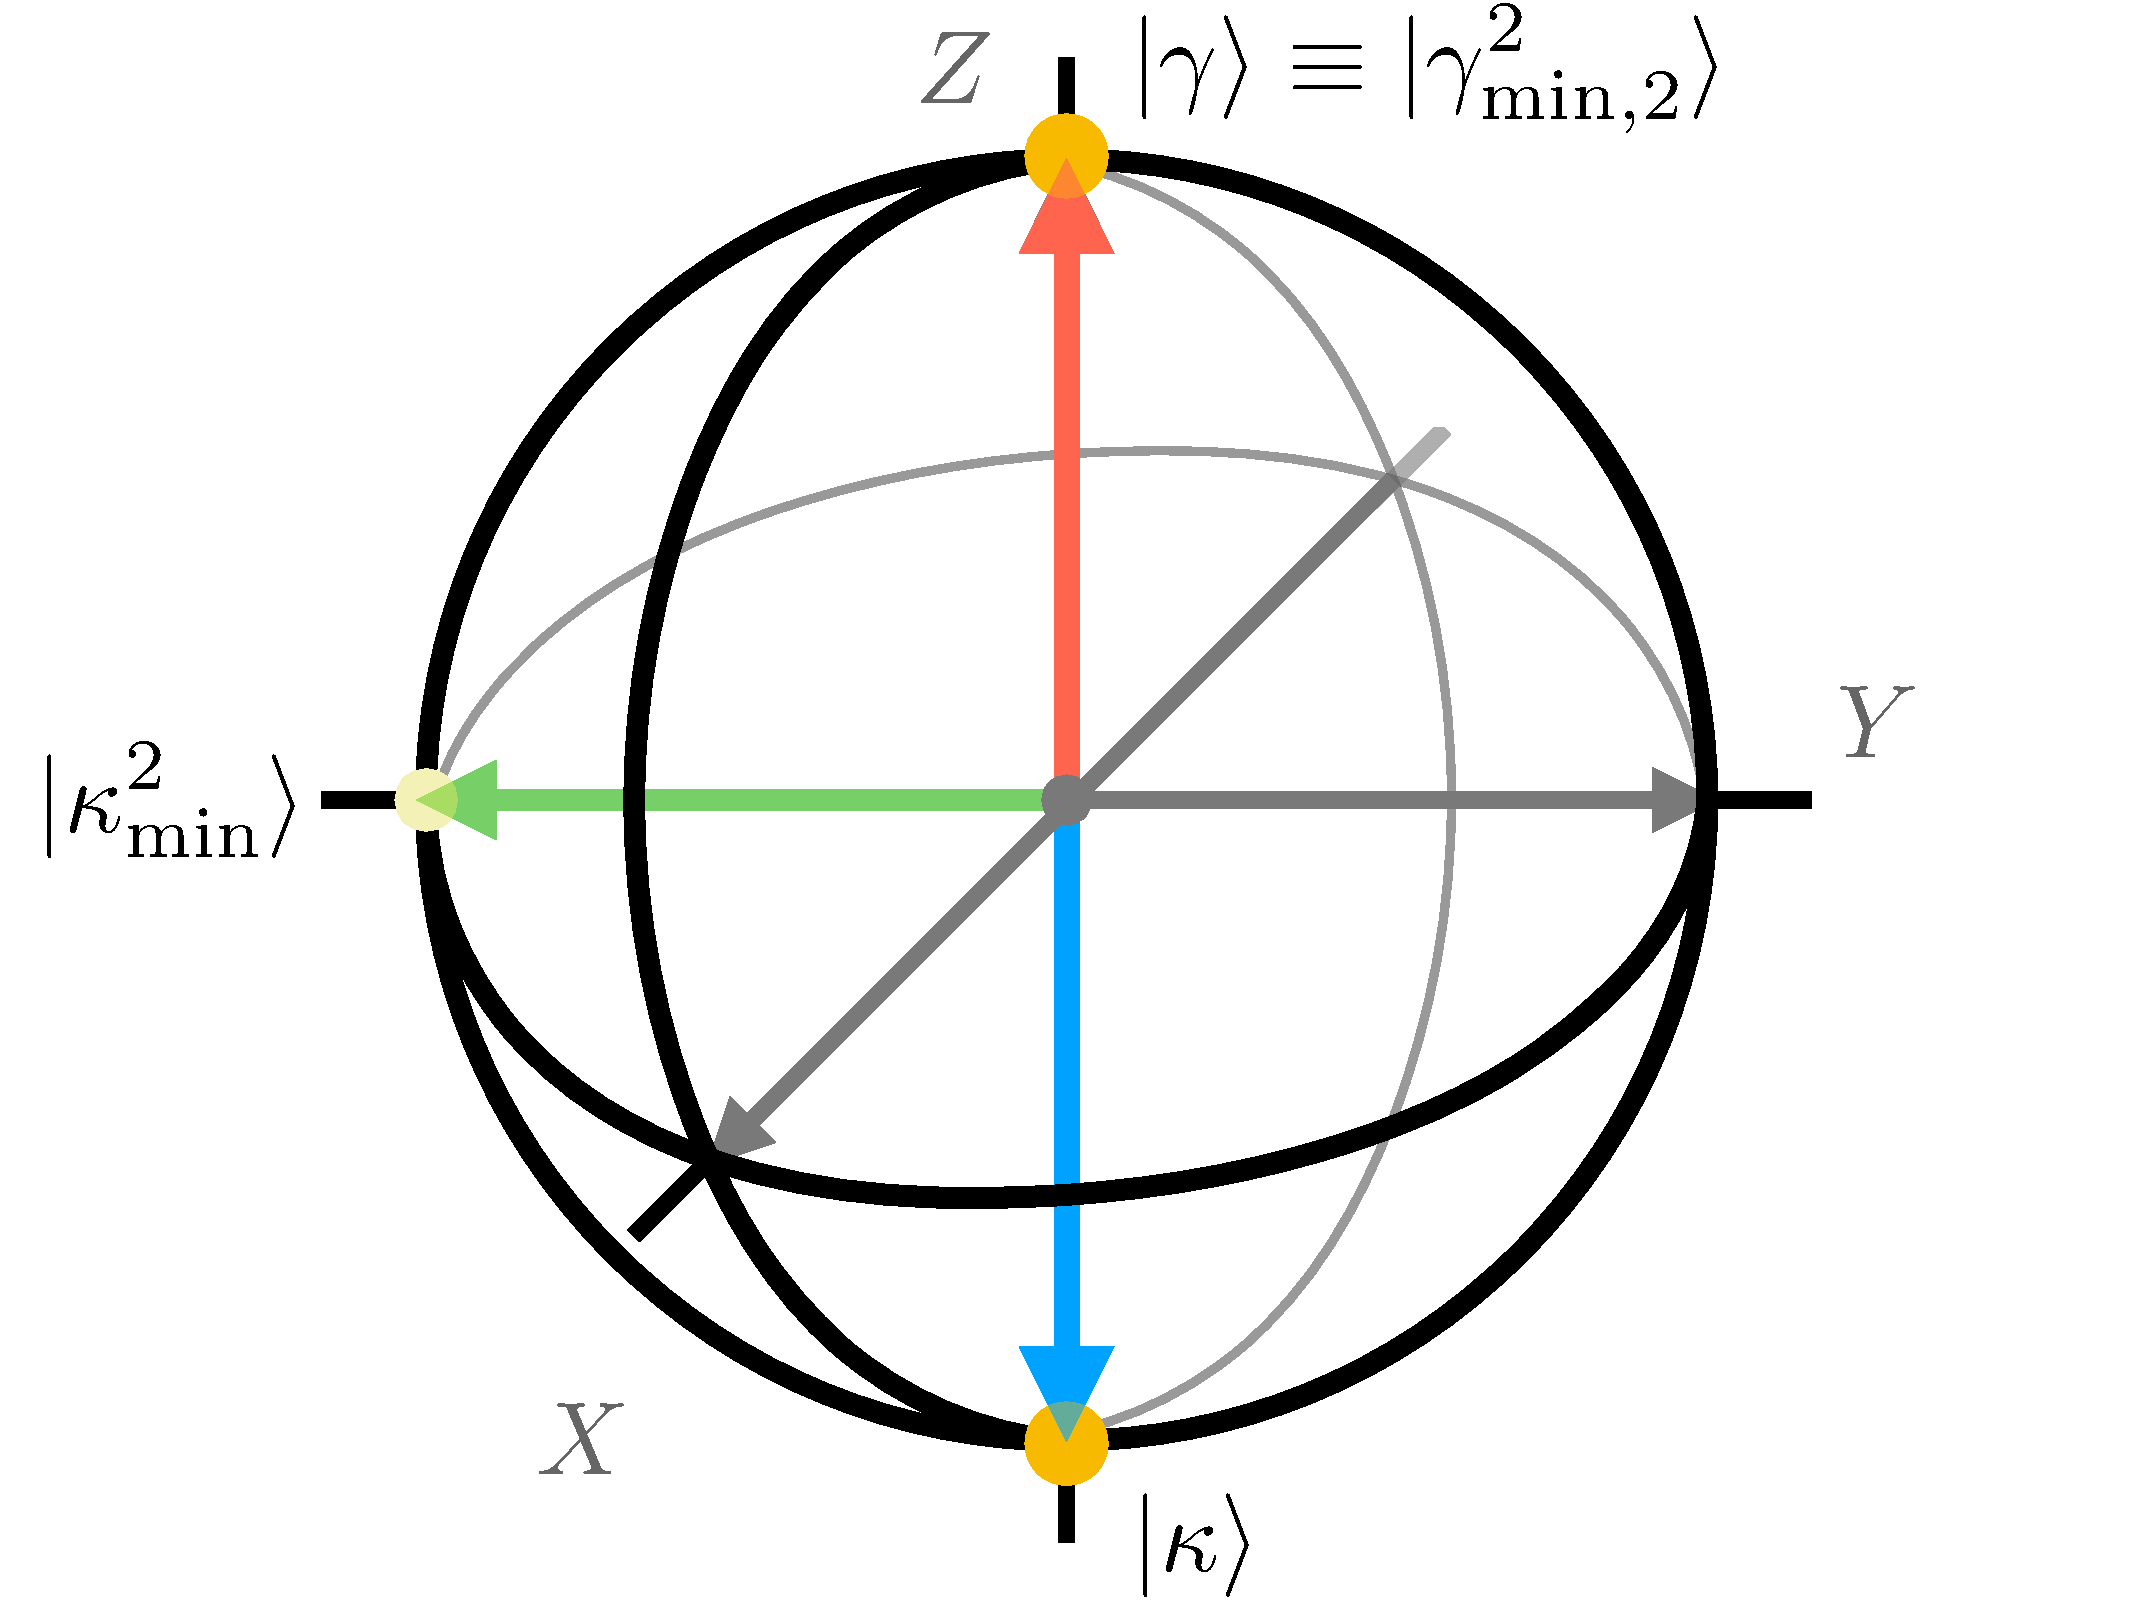
\includegraphics[width=.4\paperwidth]{Figures/NJL1-model-solving/bloch-sphere}
		\end{center}

	\end{multicols}

%% ----------------------------------------------------------------------------
\break
%% ----------------------------------------------------------------------------

	\begin{figure}[!p]
		\centering
		\begin{minipage}[c]{.45\linewidth}
			\centering
			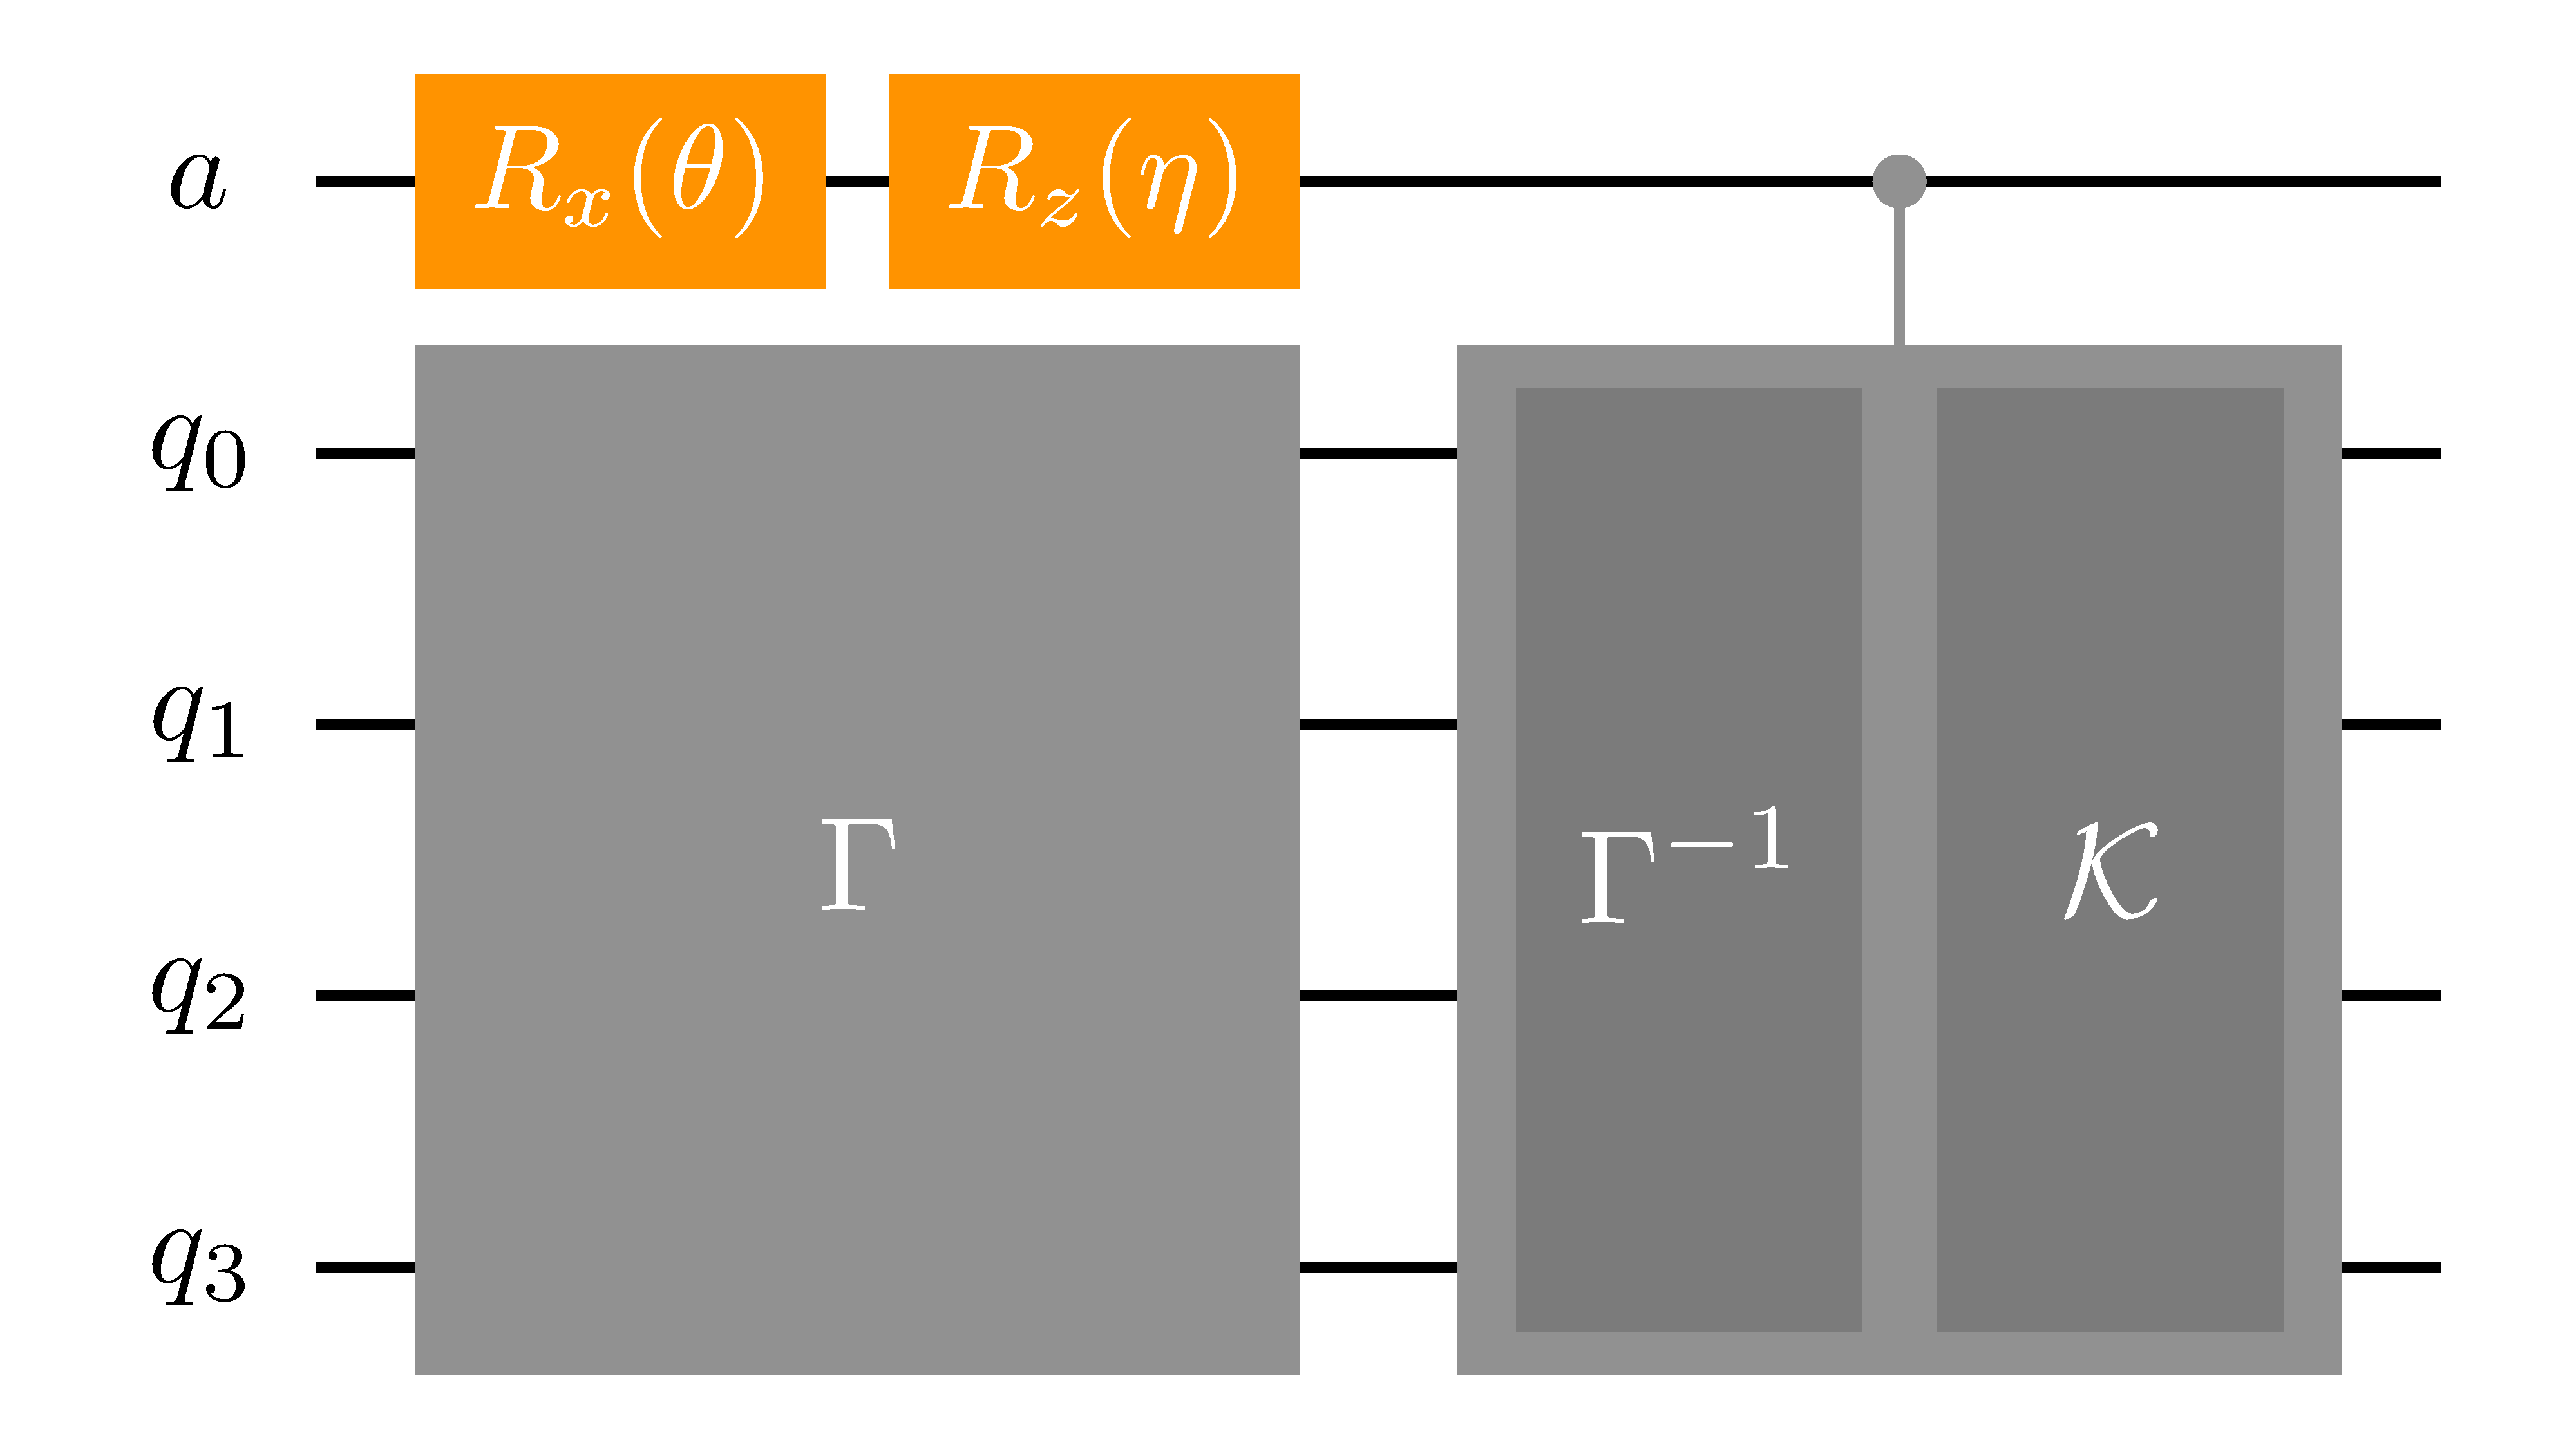
\includegraphics[width=\linewidth]{Figures/NJL1-model-solving/ansatz-implementation-ancilla-mapping}
		\end{minipage}
		\hspace{.025\linewidth}
		\begin{minipage}[c]{.45\linewidth}
			\centering
			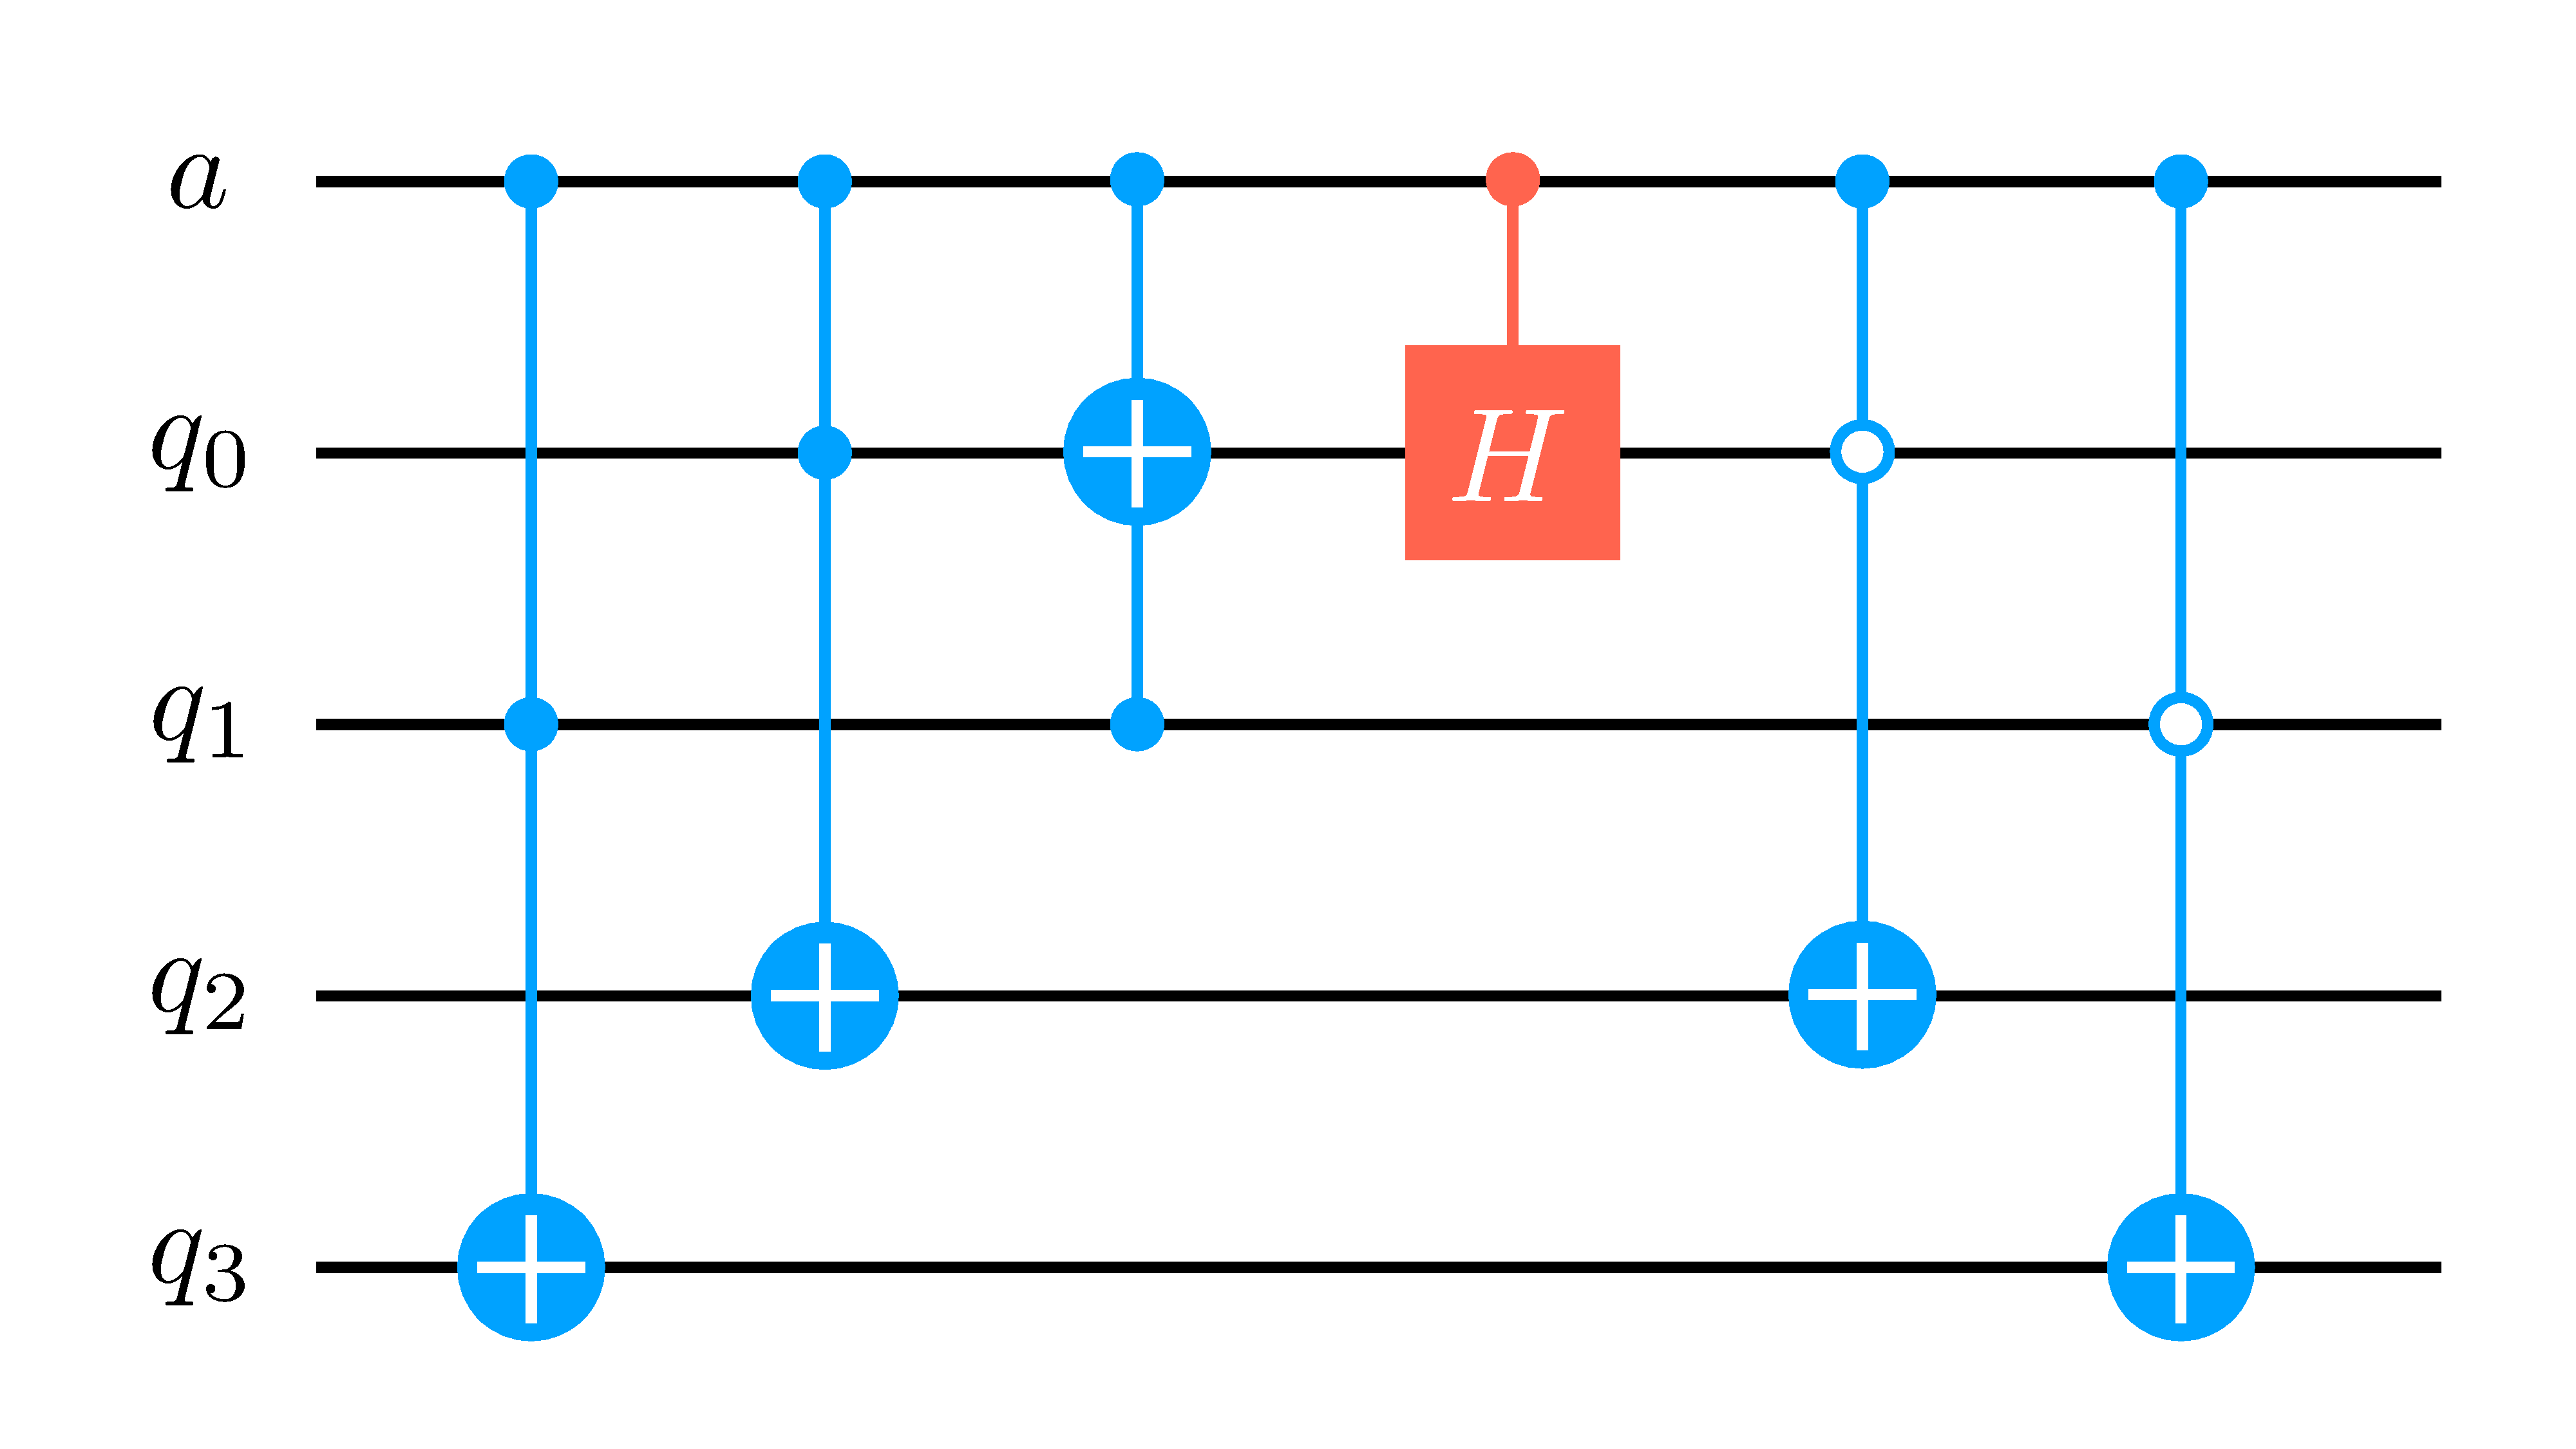
\includegraphics[width=\linewidth]{Figures/NJL1-model-solving/ansatz-implementation-controlled-gammakappa}
		\end{minipage}
		\caption{(Left) Quantum circuit to map the ancilla qubit onto the target qubit Hilbert space in our system. (Right) Simplified controlled $\mathcal{K}\Gamma^{-1}$ gate.}
	\end{figure}

%% ----------------------------------------------------------------------------
\break
%% ----------------------------------------------------------------------------

	\begin{figure}[!p]
		\centering
		\begin{minipage}[c]{.45\linewidth}
			\centering
			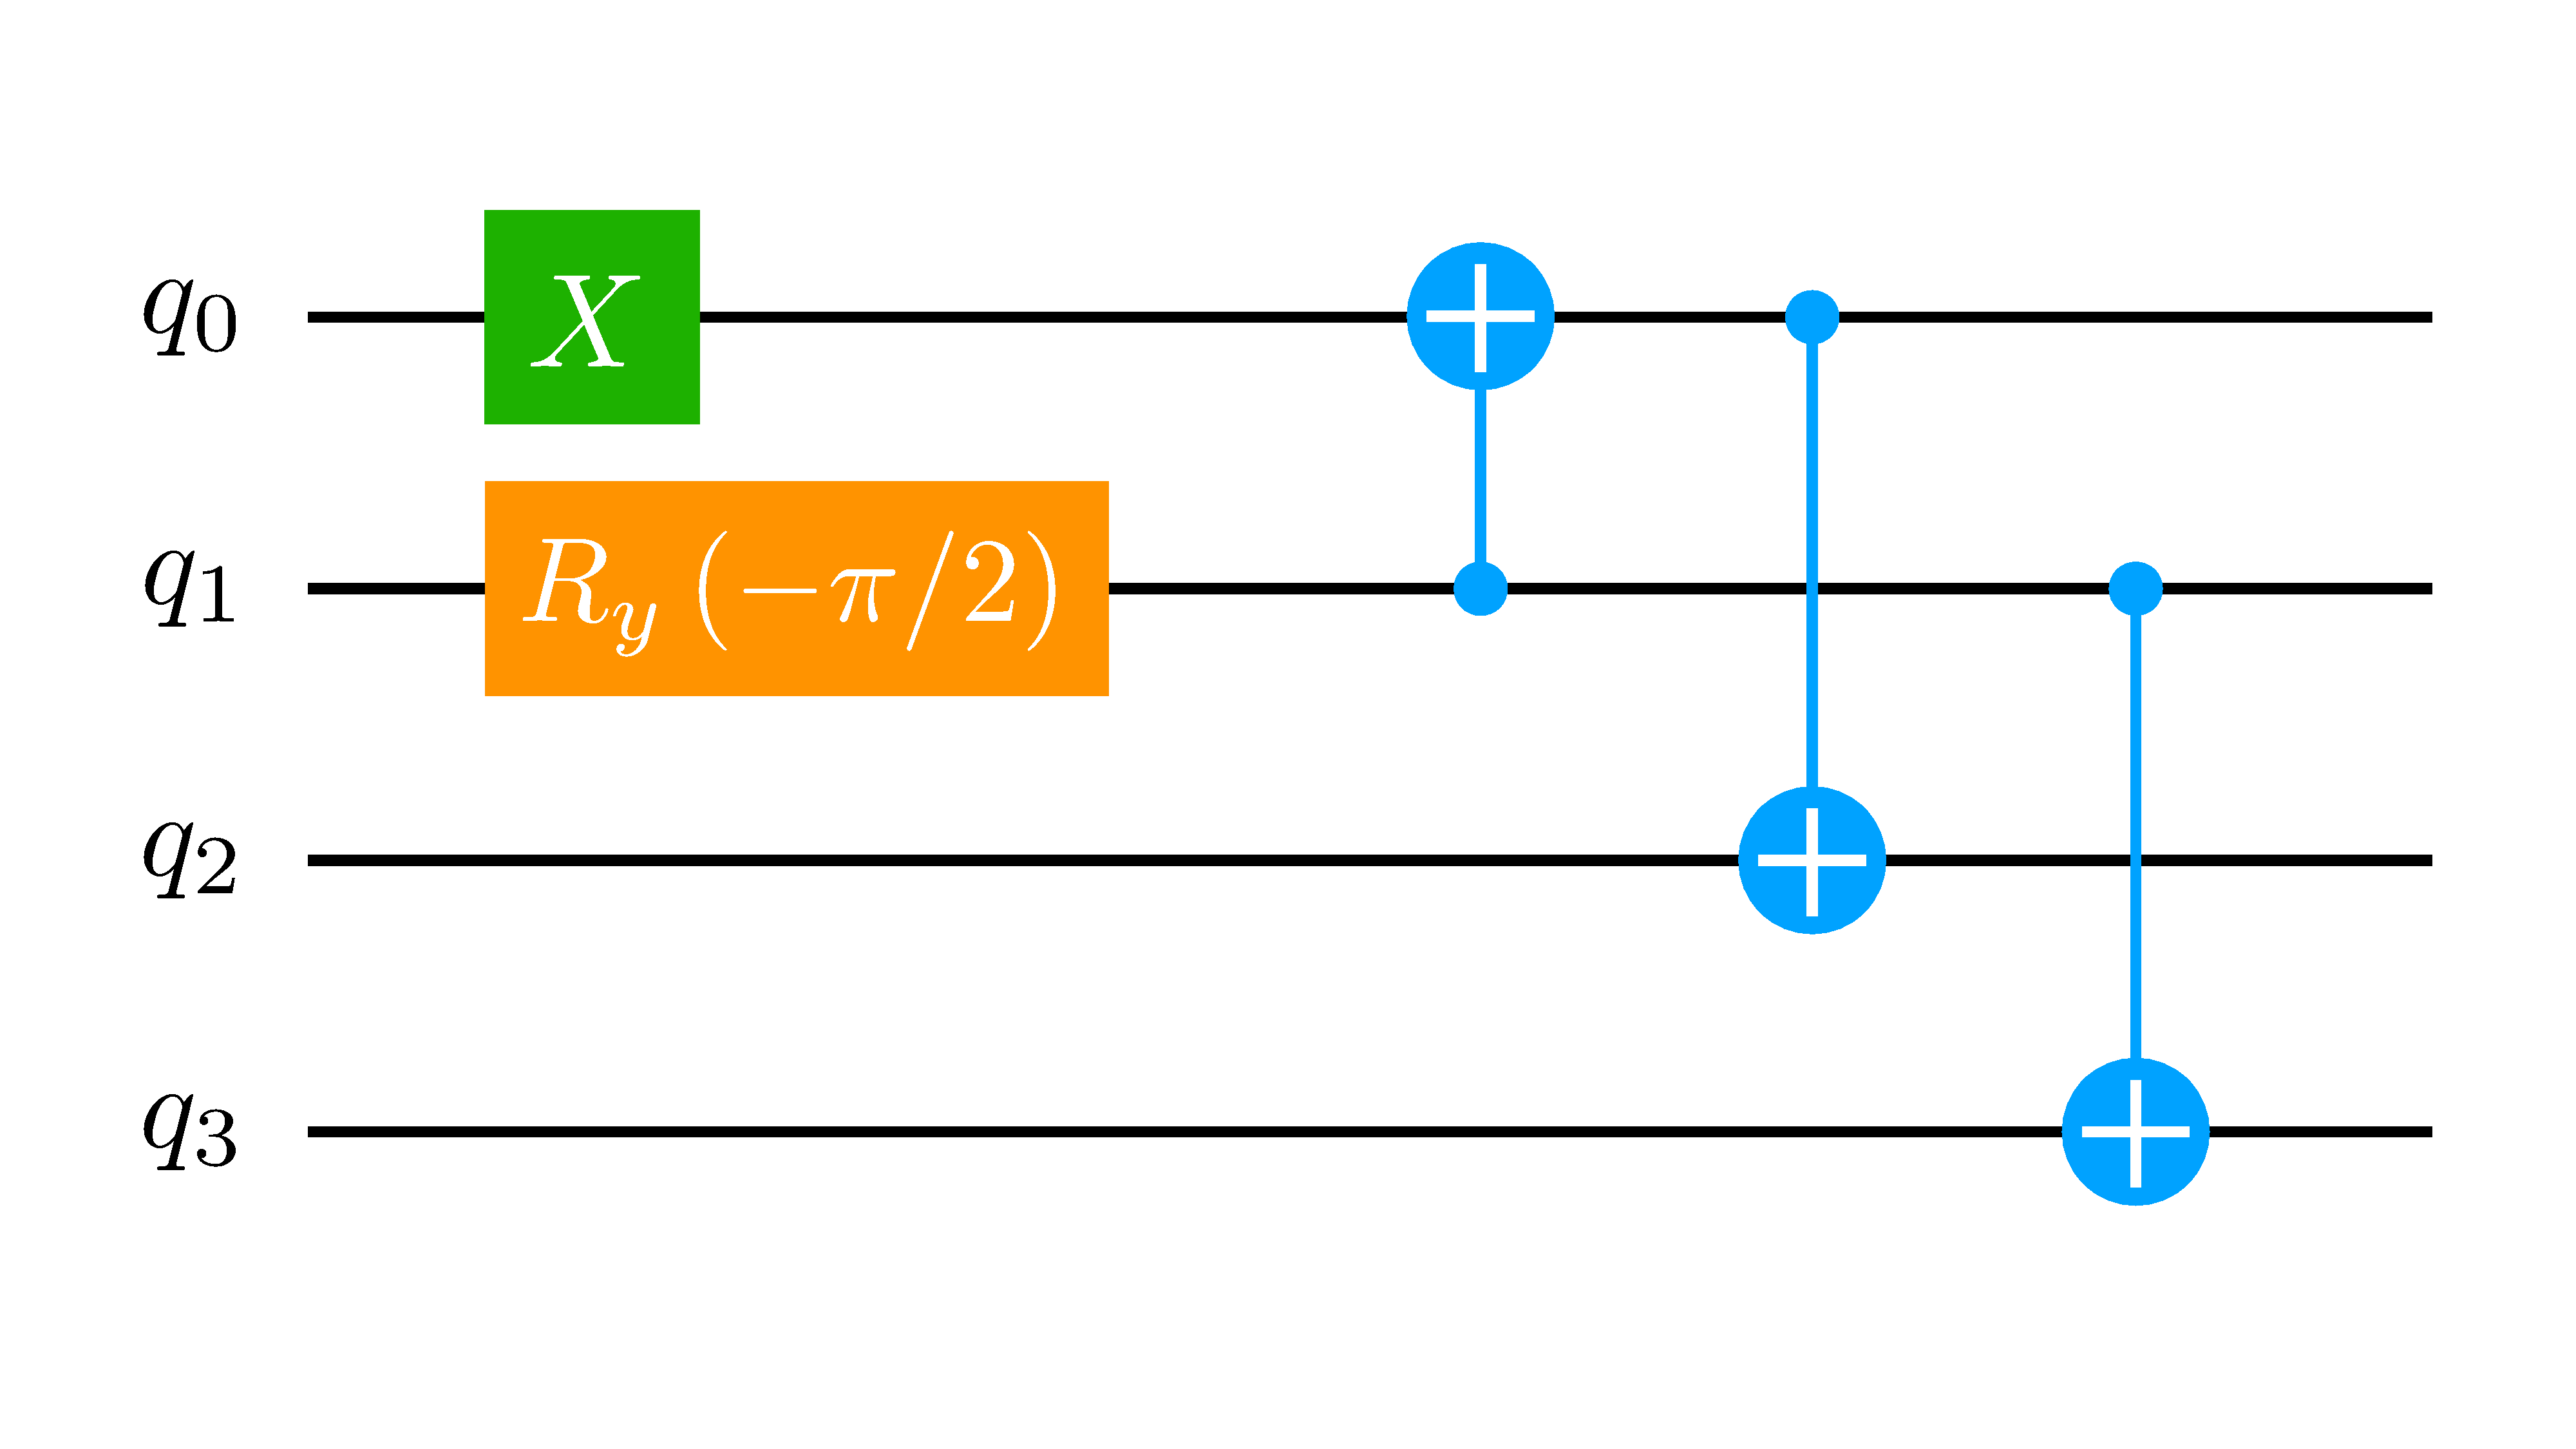
\includegraphics[width=\linewidth]{Figures/NJL1-model-solving/ansatz-implementation-base-state-preparation-gamma}
		\end{minipage}
	  \hspace{.025\linewidth}
		\begin{minipage}[c]{.45\linewidth}
			\centering
			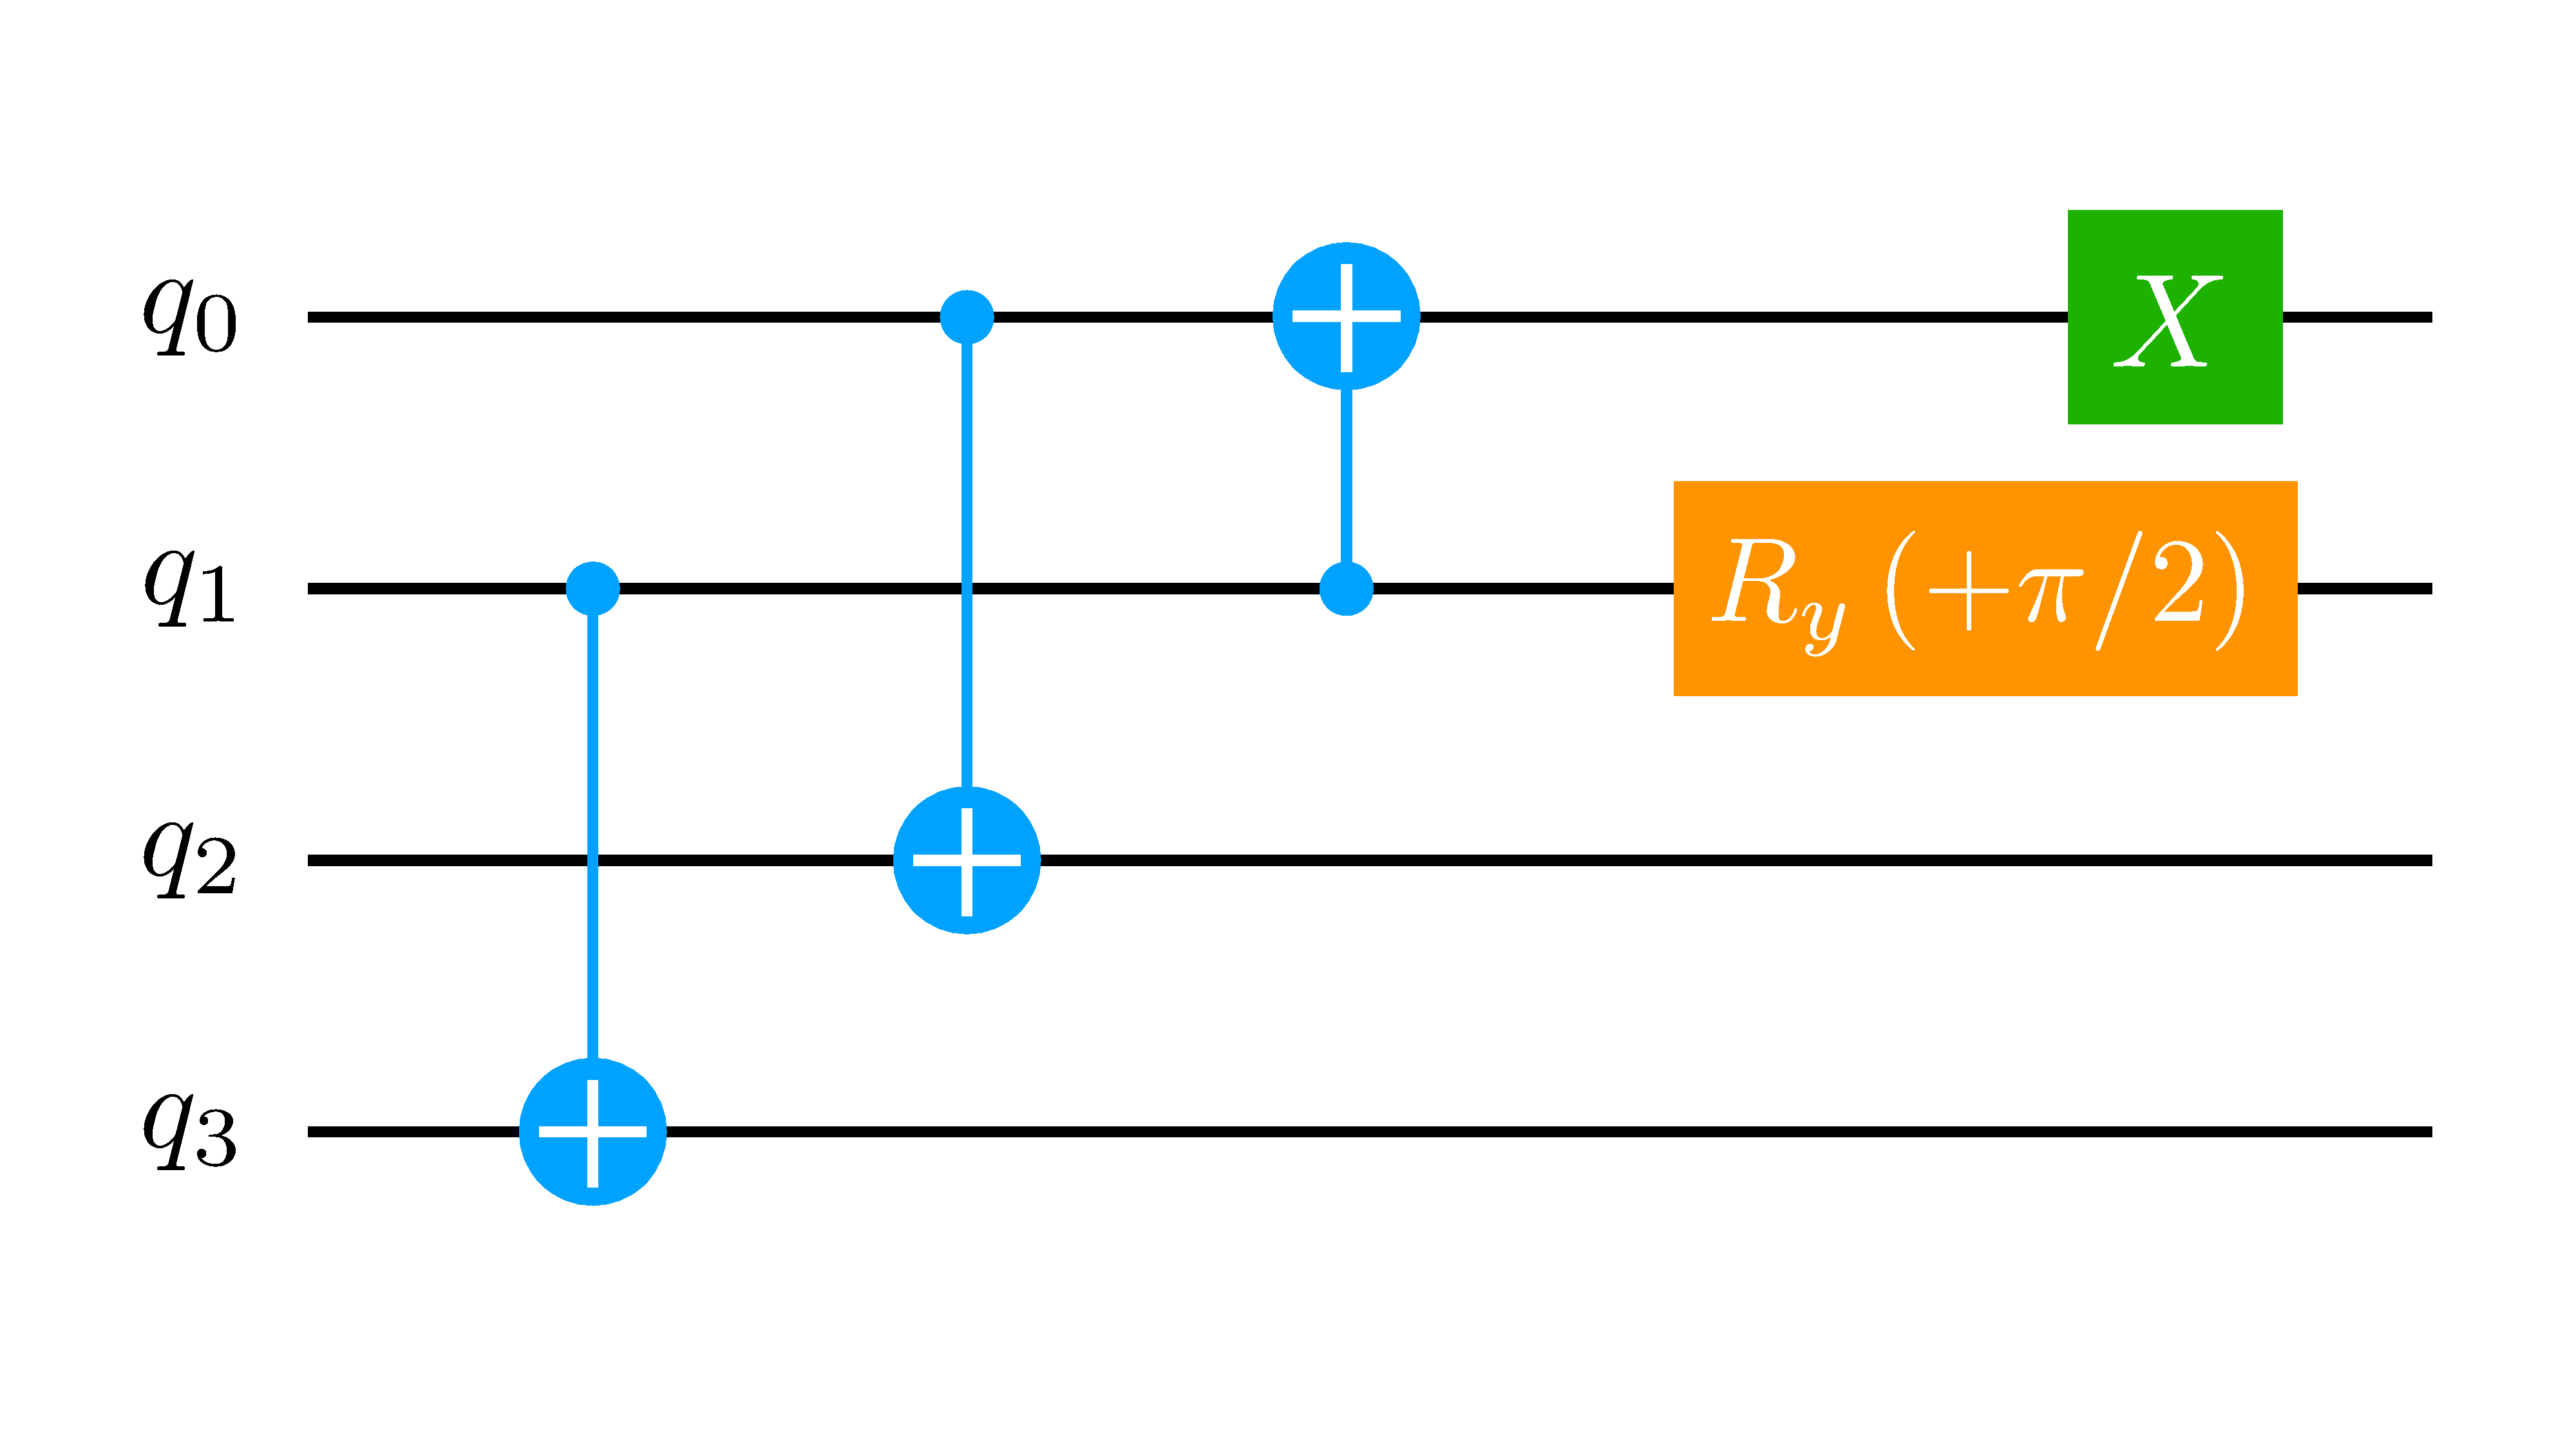
\includegraphics[width=\linewidth]{Figures/NJL1-model-solving/ansatz-implementation-base-state-reversing-gamma}
		\end{minipage}
		\caption{(Left) Preparation $\Gamma$ of state $\ket{\gamma}$. (Right) Quantum gate $\Gamma^{-1}$ for reversing state $\ket{\gamma}$.}
	\end{figure}

%% ----------------------------------------------------------------------------
\break
%% ----------------------------------------------------------------------------

	\begin{figure}[!p]
		\centering
		\begin{minipage}[c]{.45\linewidth}
			\centering
			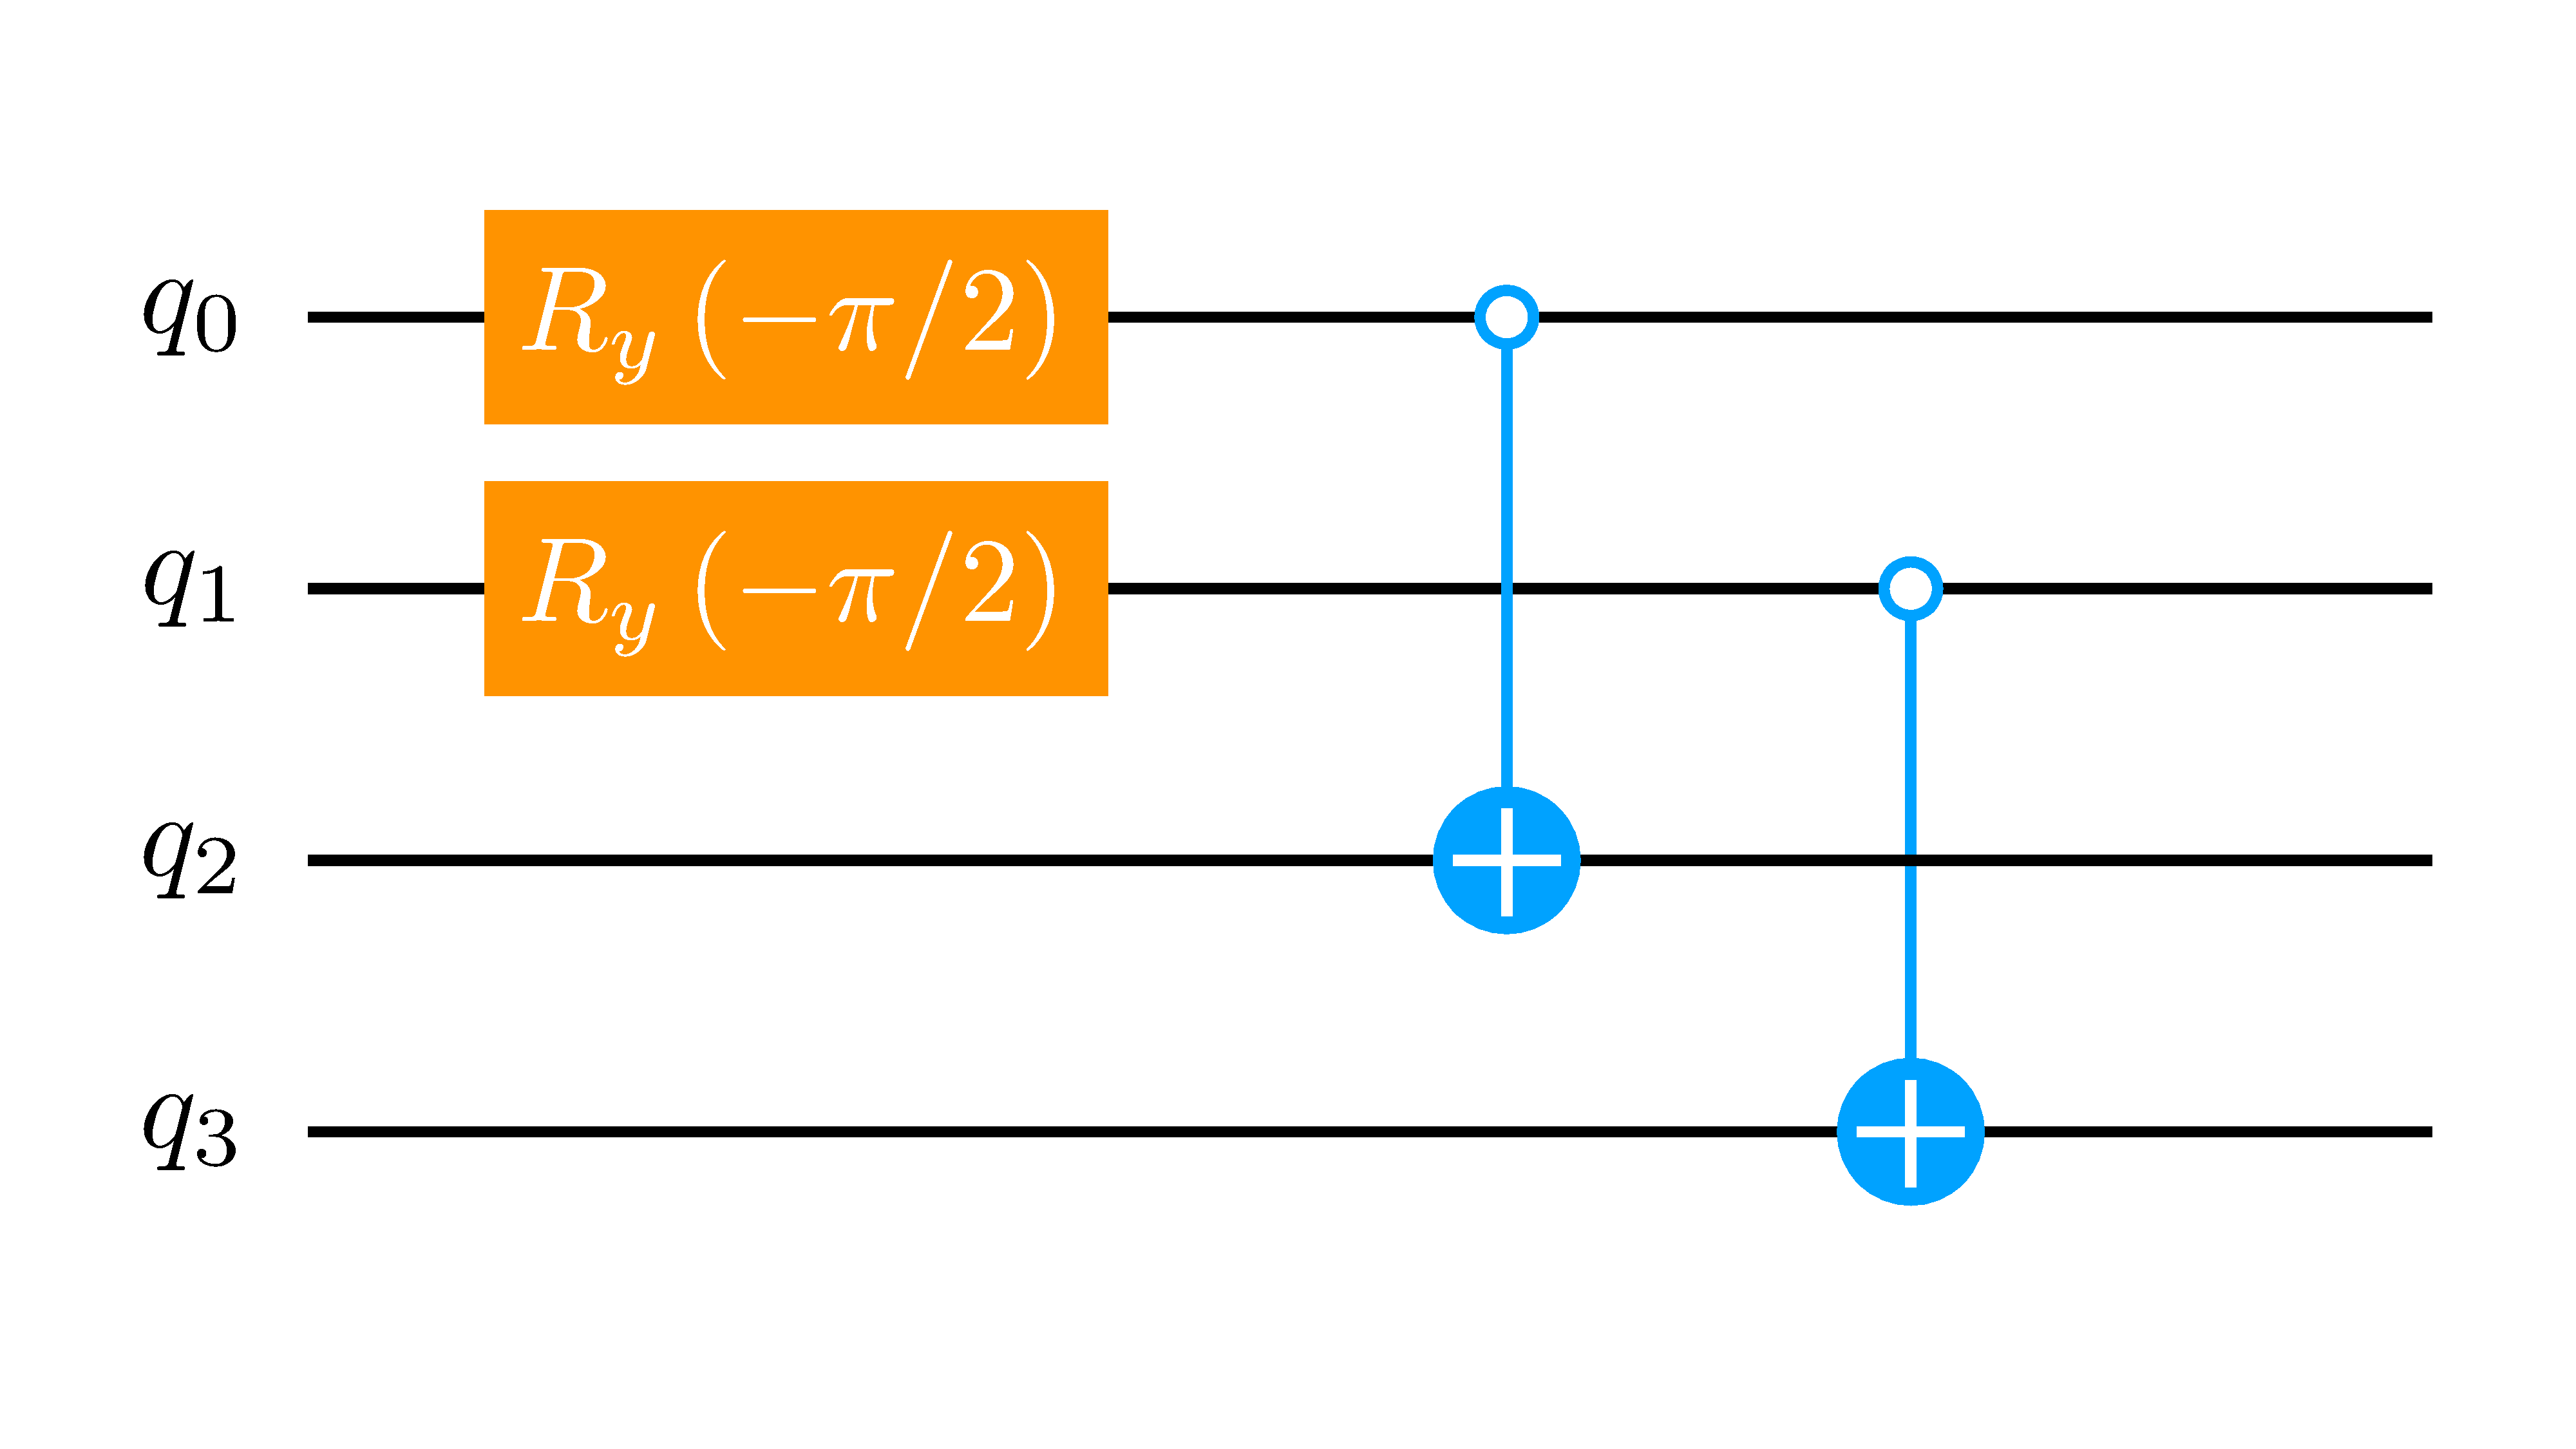
\includegraphics[width=\linewidth]{Figures/NJL1-model-solving/ansatz-implementation-base-state-preparation-kappa}
		\end{minipage}
	  \hspace{.025\linewidth}
		\begin{minipage}[c]{.45\linewidth}
			\centering
			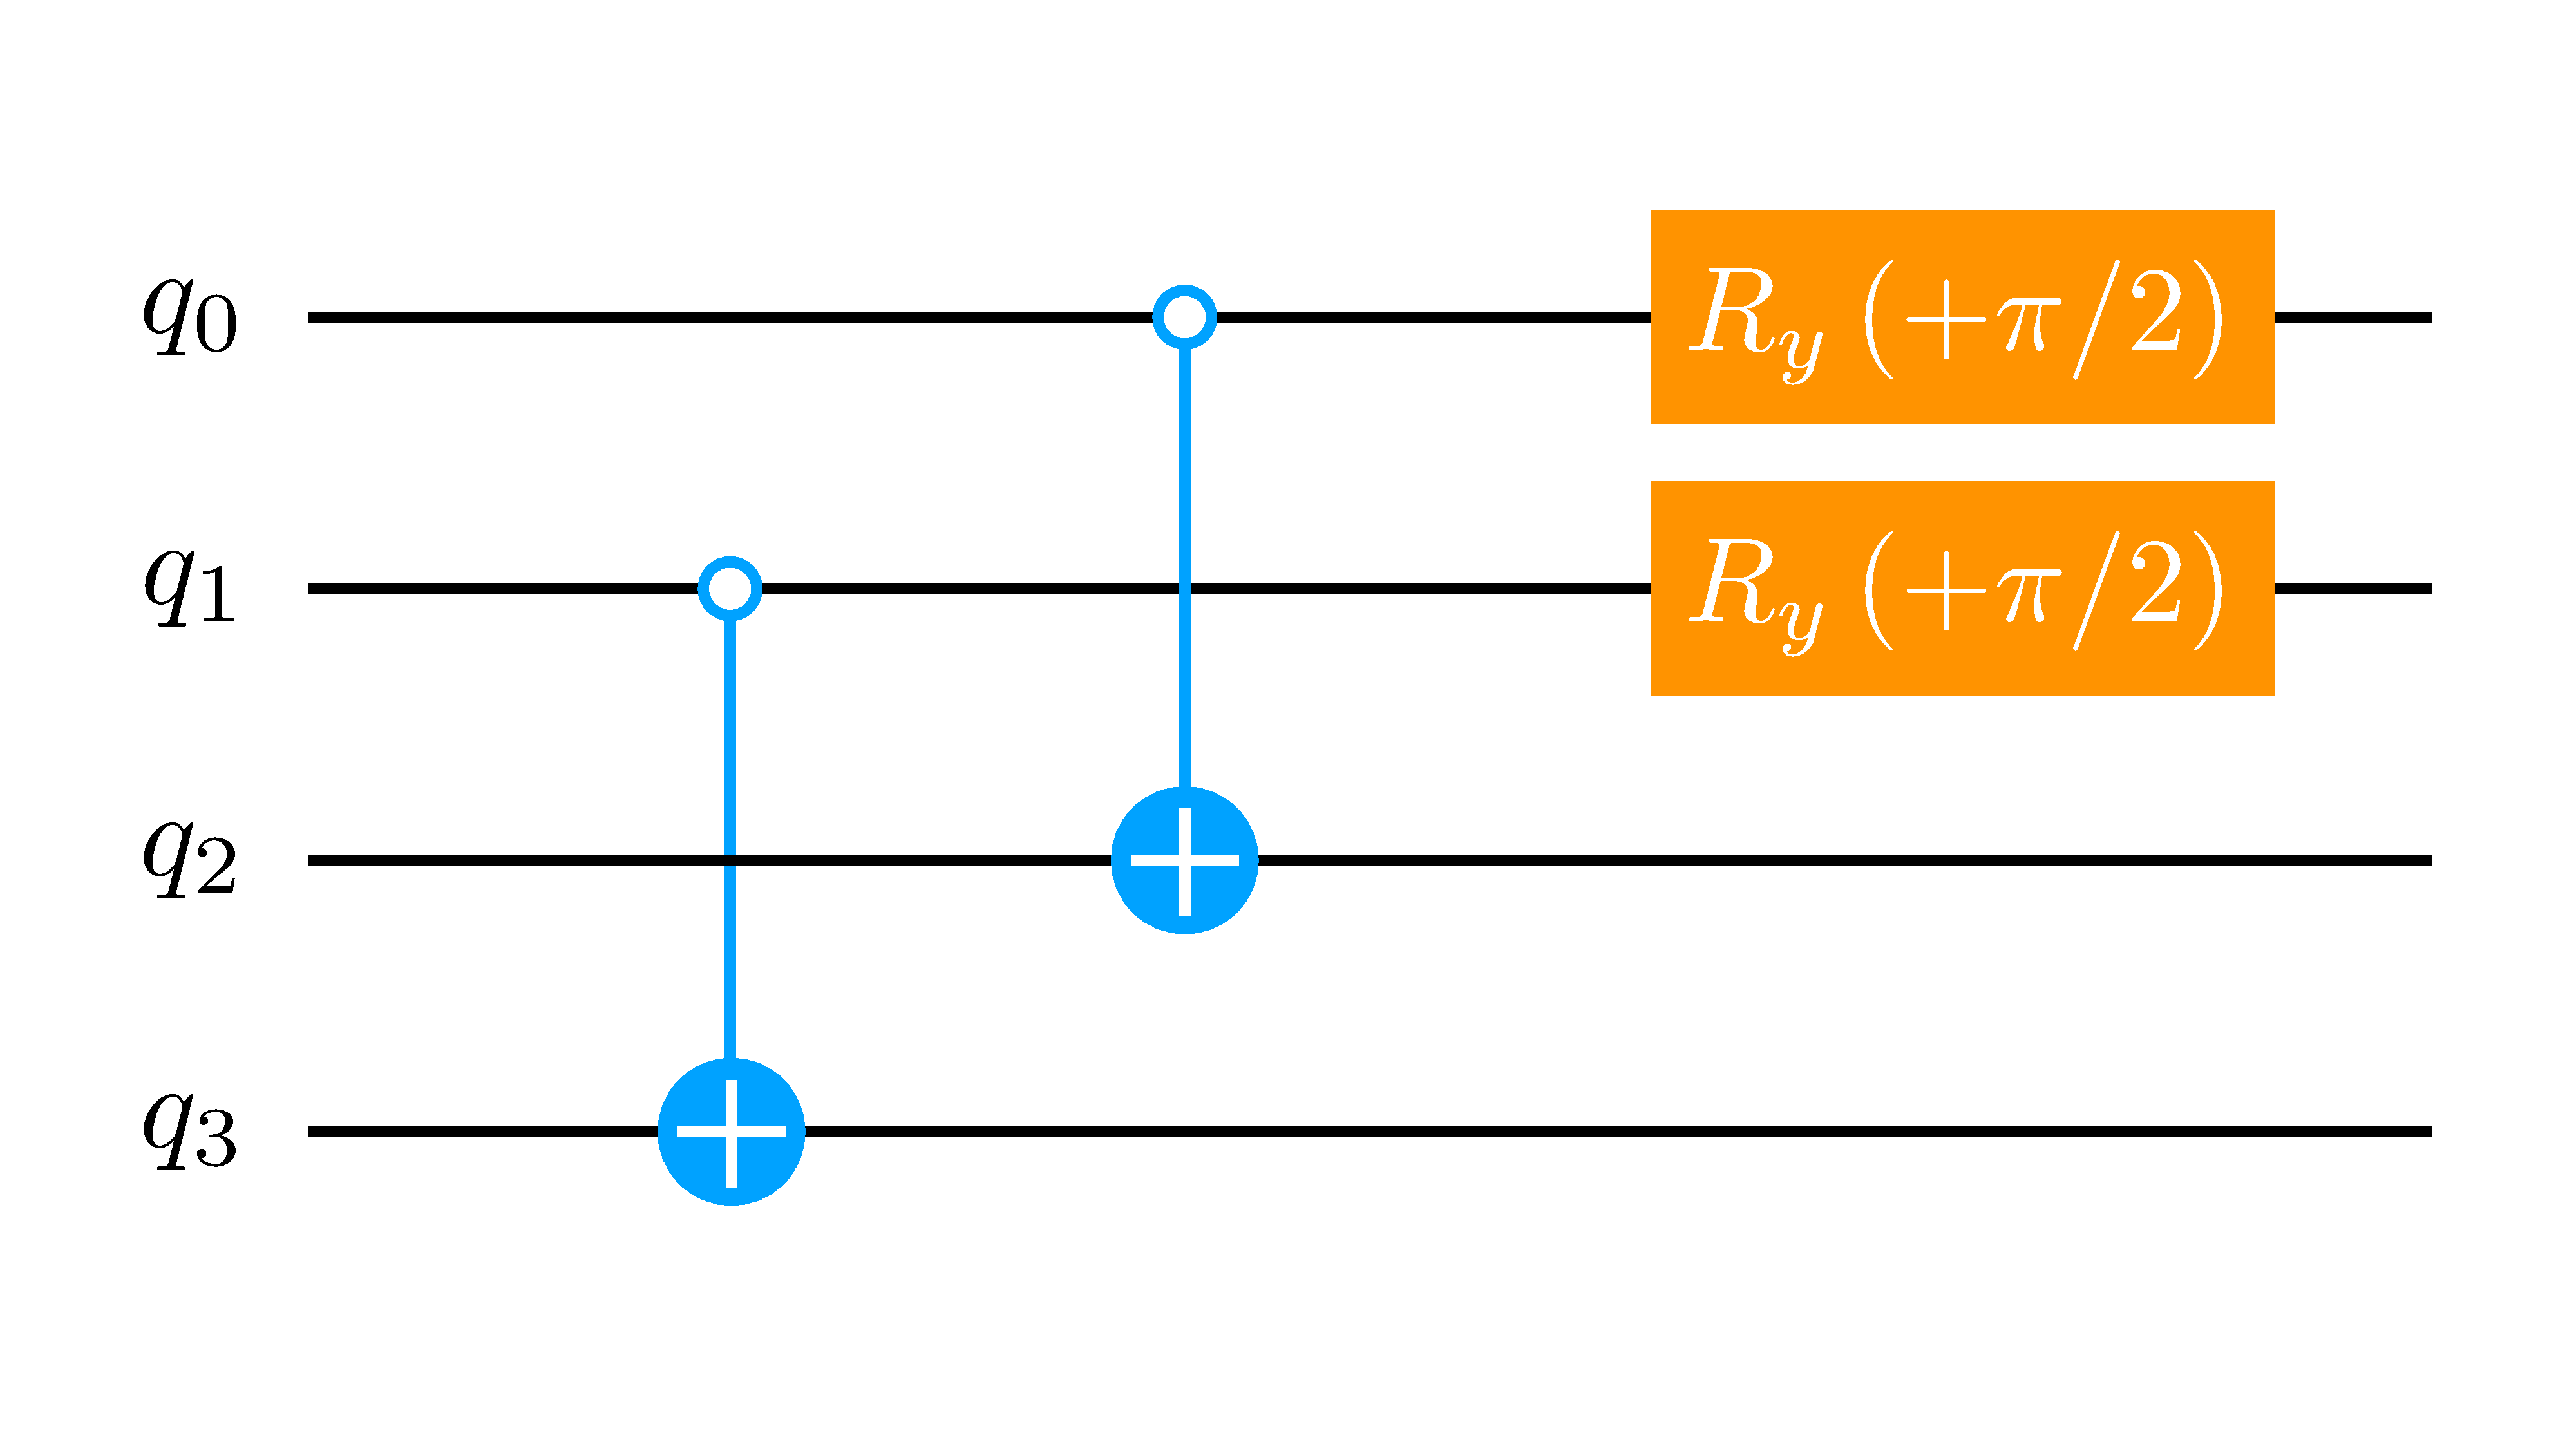
\includegraphics[width=\linewidth]{Figures/NJL1-model-solving/ansatz-implementation-base-state-reversing-kappa}
		\end{minipage}
		\caption{(Left) Preparation $\mathcal{K}$ of state $\ket{\kappa}$. (Right) Quantum gate $\mathcal{K}^{-1}$ for reversing state $\ket{\kappa}$.}
	\end{figure}

%% ----------------------------------------------------------------------------
\break
%% ----------------------------------------------------------------------------

	\begin{multicols}{2}

		This parametrization will work if we are interested in measuring in the computational basis only (i.e. Pauli-Z measurements). Nonetheless, if we change our basis before measuring (e.g. to Pauli-X or Pauli-Y) we are going to face a problem: the resulting states of our system will be entangled with the ancilla qubit, and so, states that should be indistinguishable from one another will turn out distinct; because of this, the probability distributions will not be correct.

		\begin{gather*}
		  \text{Pr} \qty(\ket{\psi}_{\text{distinct}}) =
		    \norm{\psi_\gamma}^2 + \norm{\psi_\kappa}^2 \\
		  \text{Pr} \qty(\ket{\psi}_{\text{indist}}) =
		    \norm{\psi_\gamma + \psi_\kappa}^2 \\
		  \text{Pr} \qty(\ket{\psi}_{\text{distinct}}) \geq
		    \text{Pr} \qty(\ket{\psi}_{\text{indist}})
		\end{gather*}

		\columnbreak

		Therefore, as a last step, we need to \textbf{break this entanglement}.

		\begin{center}
			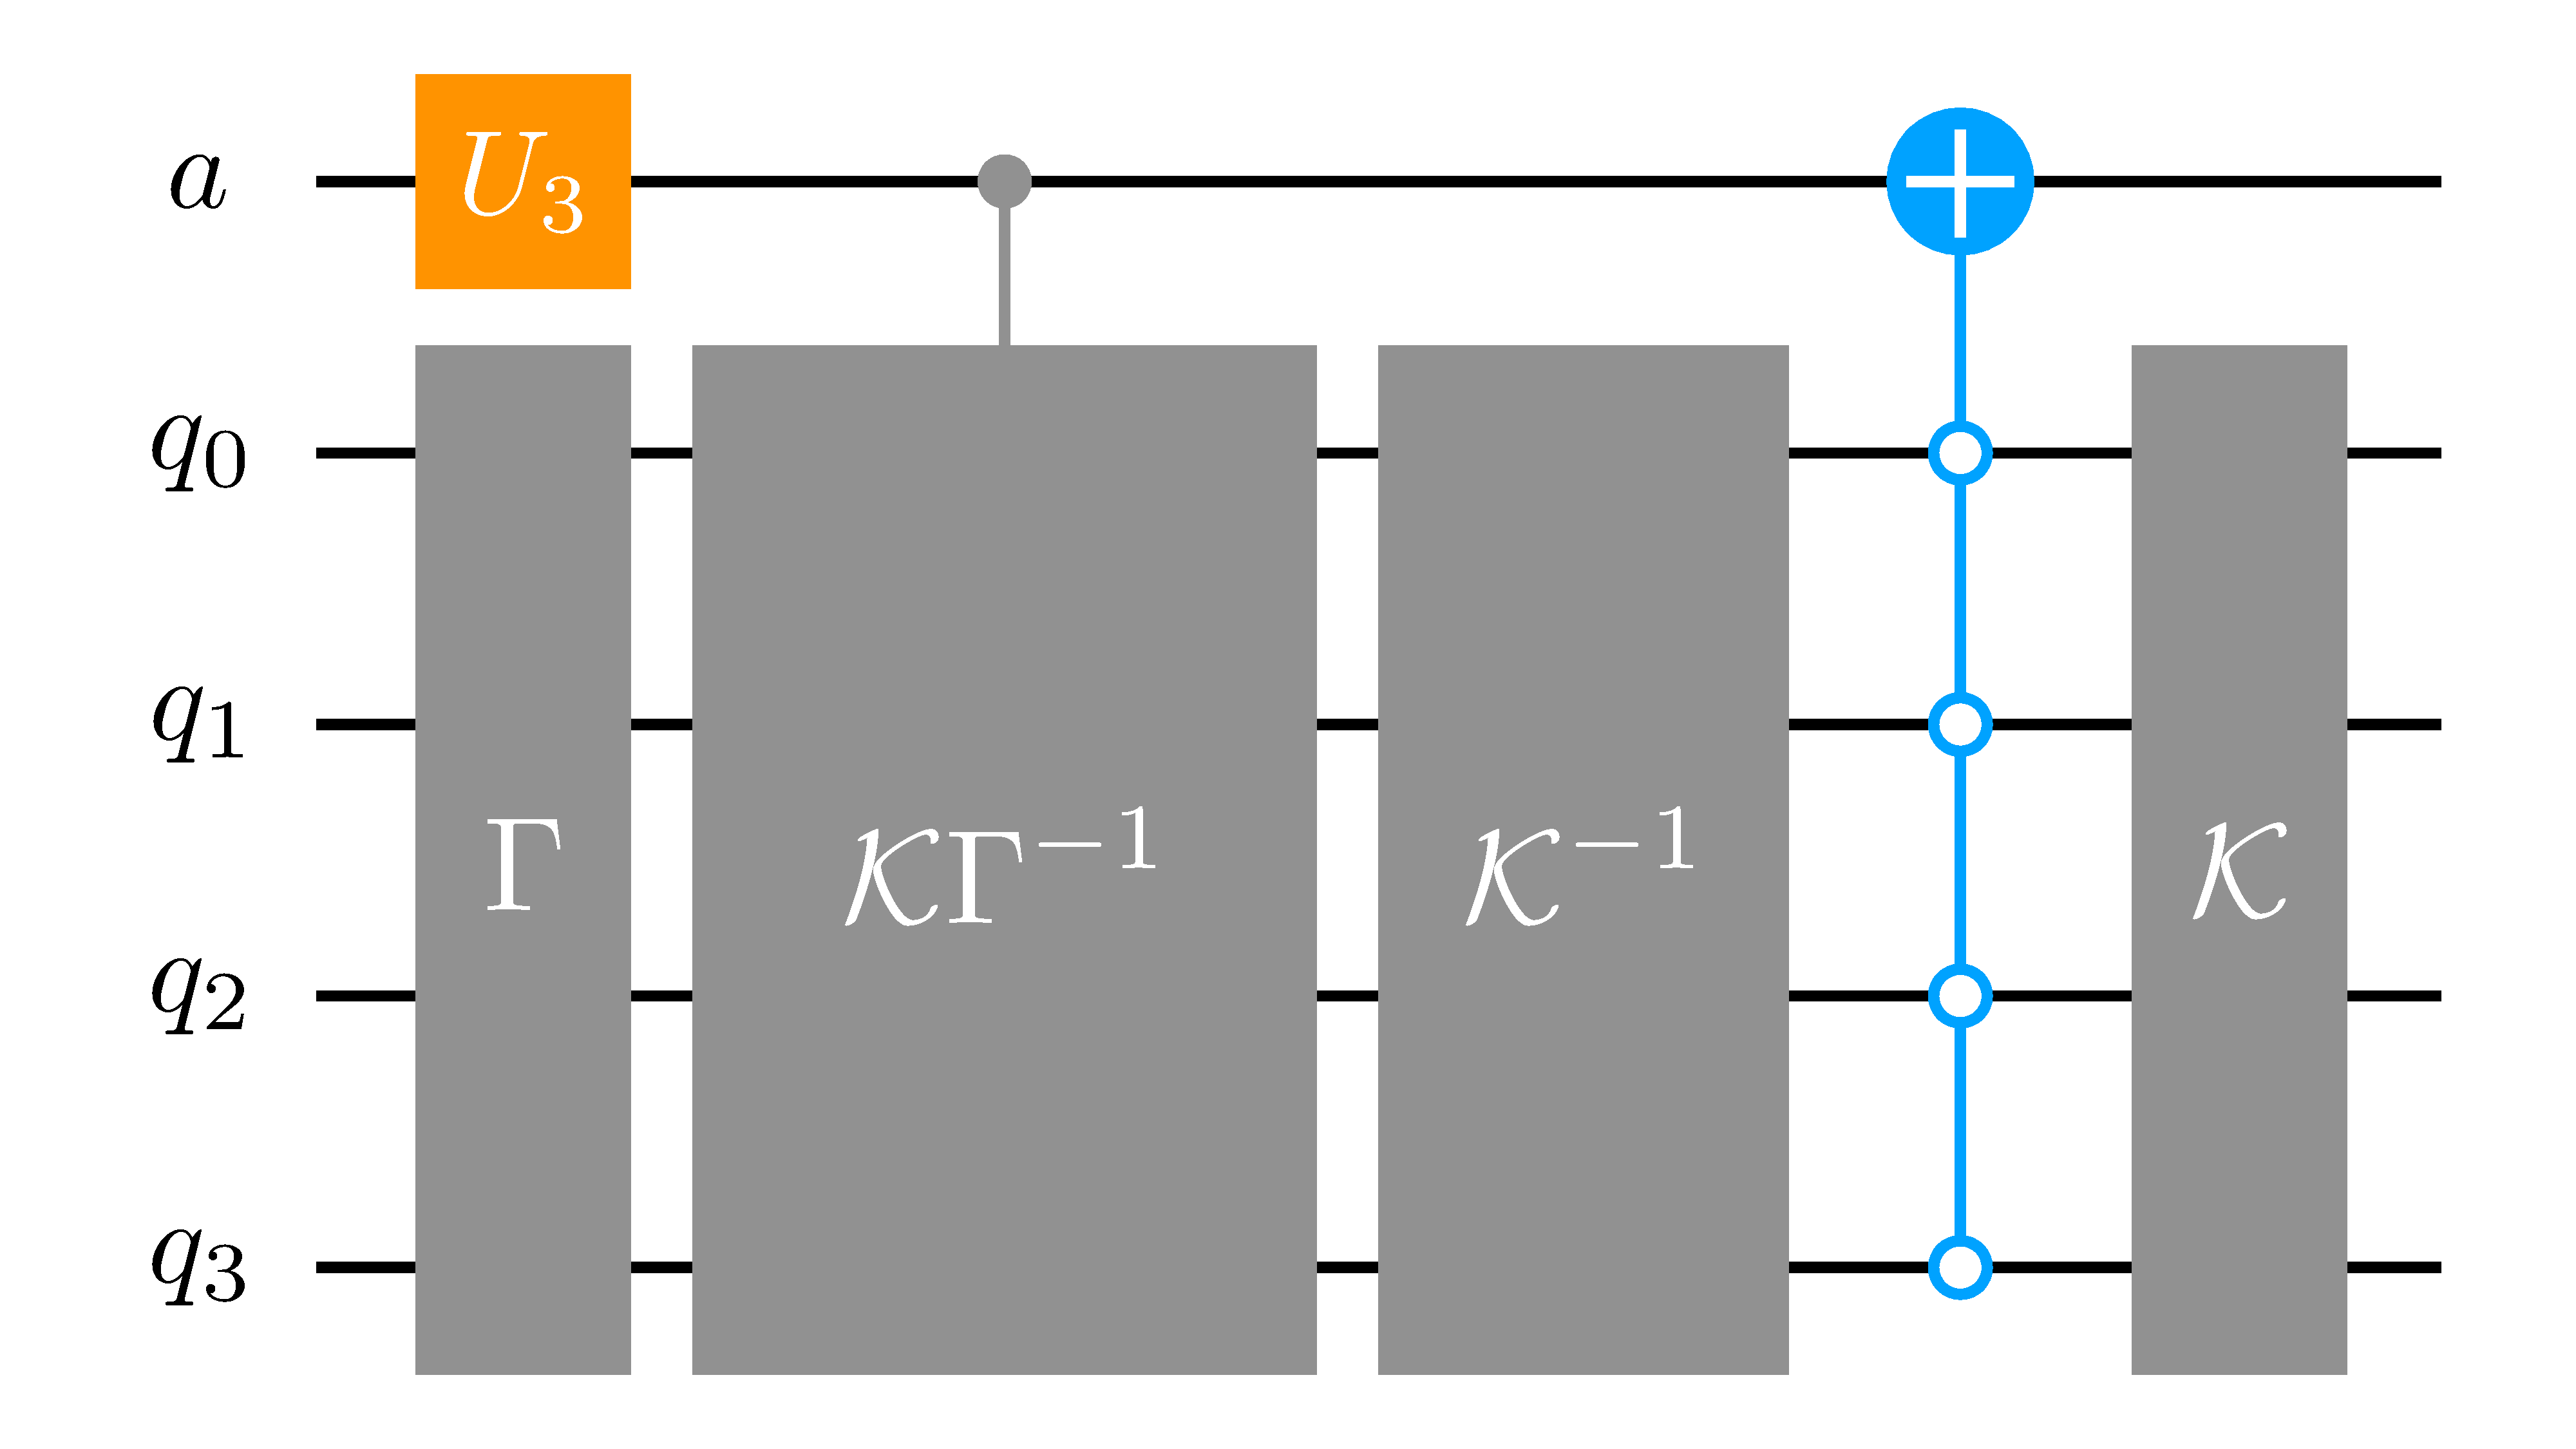
\includegraphics[width=.4\paperwidth]{Figures/NJL1-model-solving/ansatz-implementation-circuit}
		\end{center}

	\end{multicols}

\end{frame}

%% ----------------------------------------------------------------------------
%% ----------------------------------------------------------------------------

\begin{frame}[allowframebreaks]{Ground state energy}

	At long last, we have everything that we need to solve for the ground state energy of our system using a quantum computer. For simplicity, we will do so first through a \textbf{quantum simulator}.

	\begin{center}
		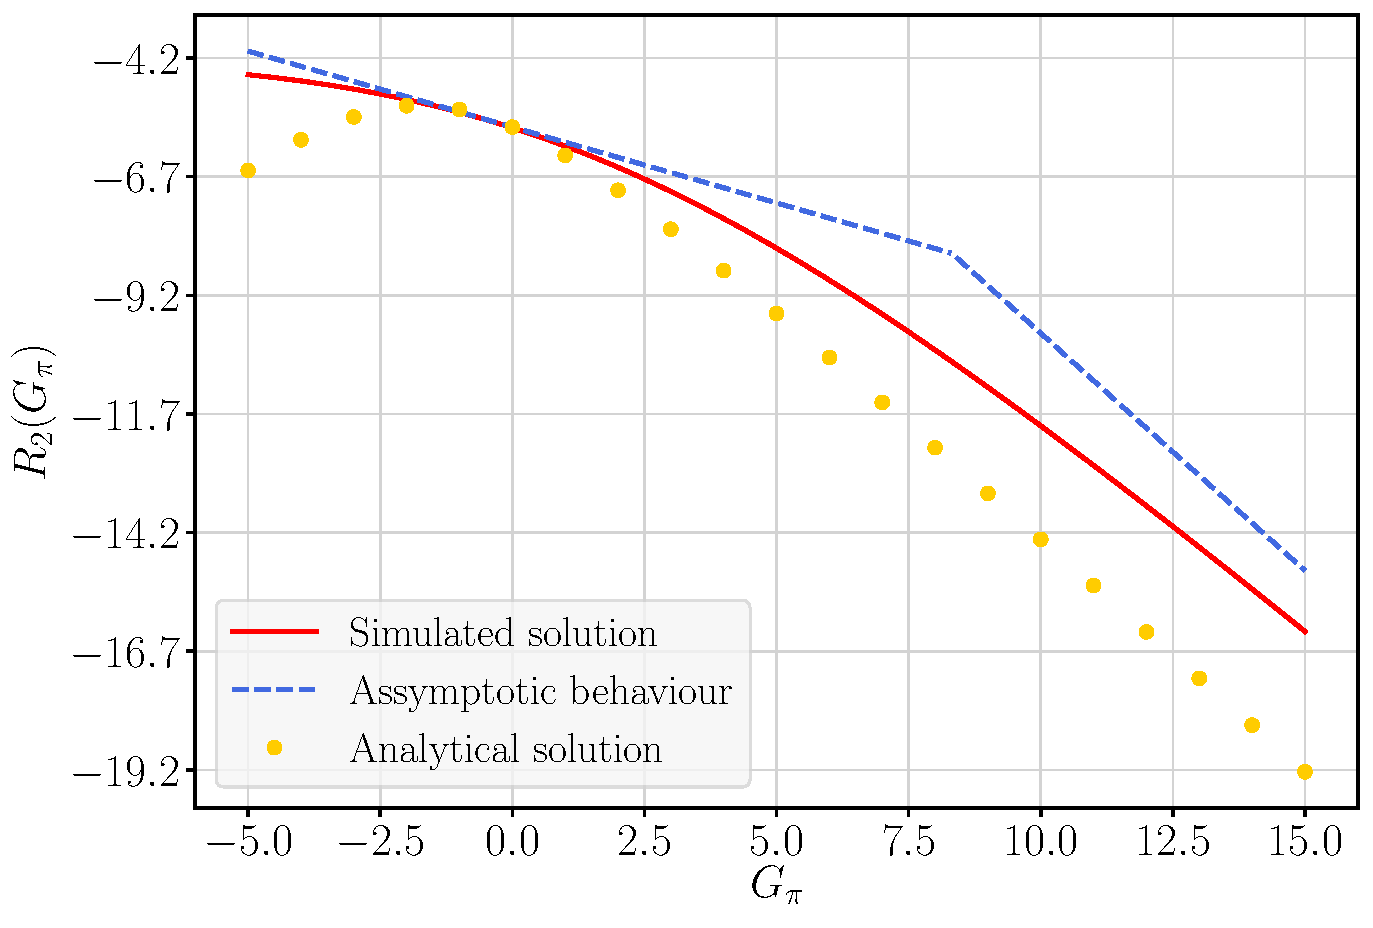
\includegraphics[width=.45\paperwidth]{Figures/chapter05/G2}
	\end{center}
	\vspace{-2em}

%% ----------------------------------------------------------------------------
\break
%% ----------------------------------------------------------------------------

	\begin{figure}[!p]
		\centering
		\begin{minipage}[c]{.4\linewidth}
			\centering
			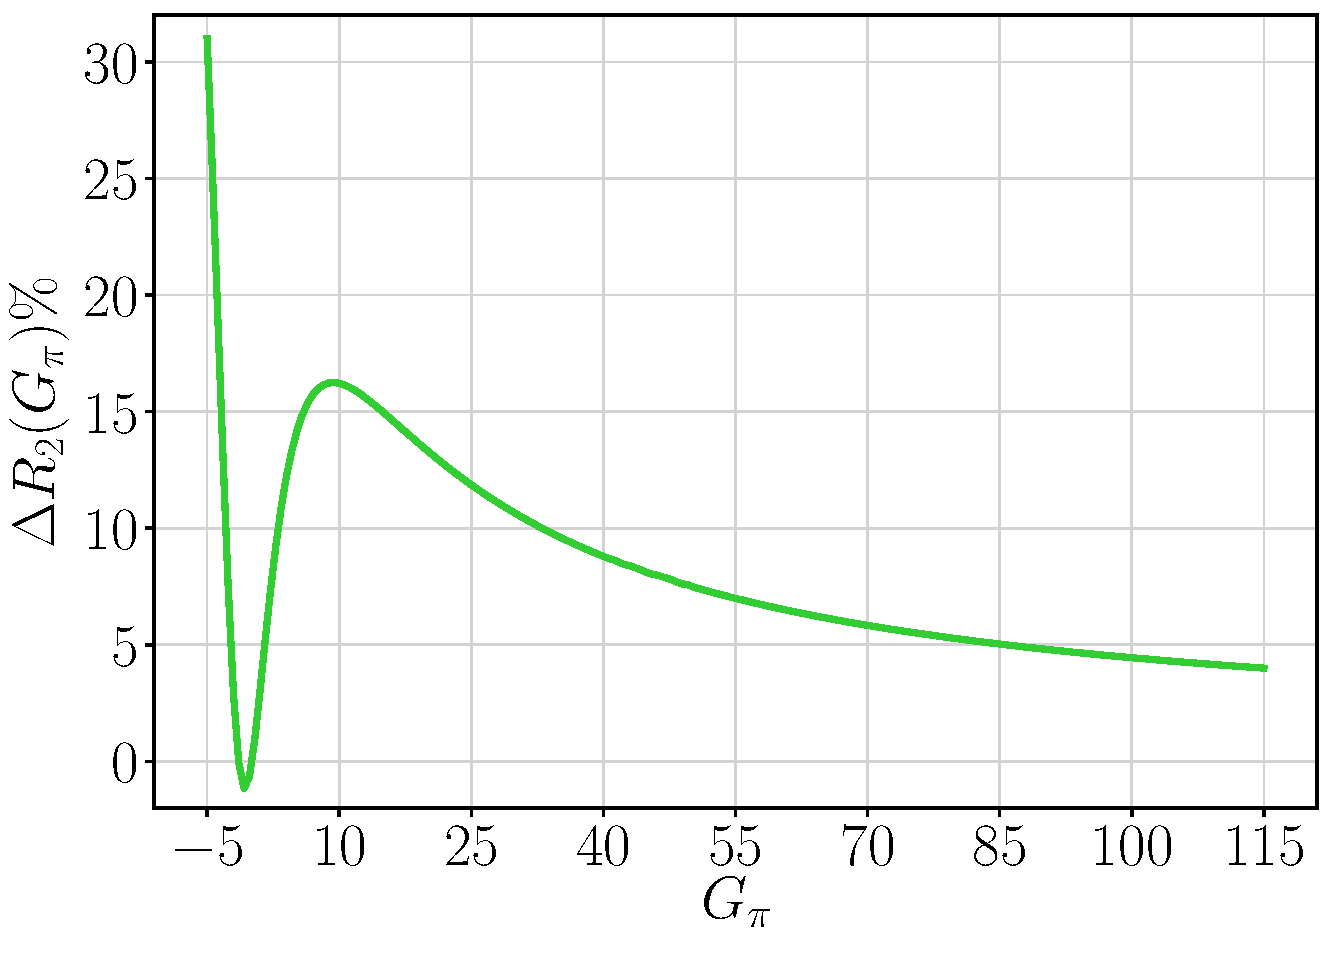
\includegraphics[width=.8\linewidth]{Figures/chapter05/G2-err}
		\end{minipage}
		\hspace{.025\linewidth}
		\begin{minipage}[c]{.4\linewidth}
			\centering
			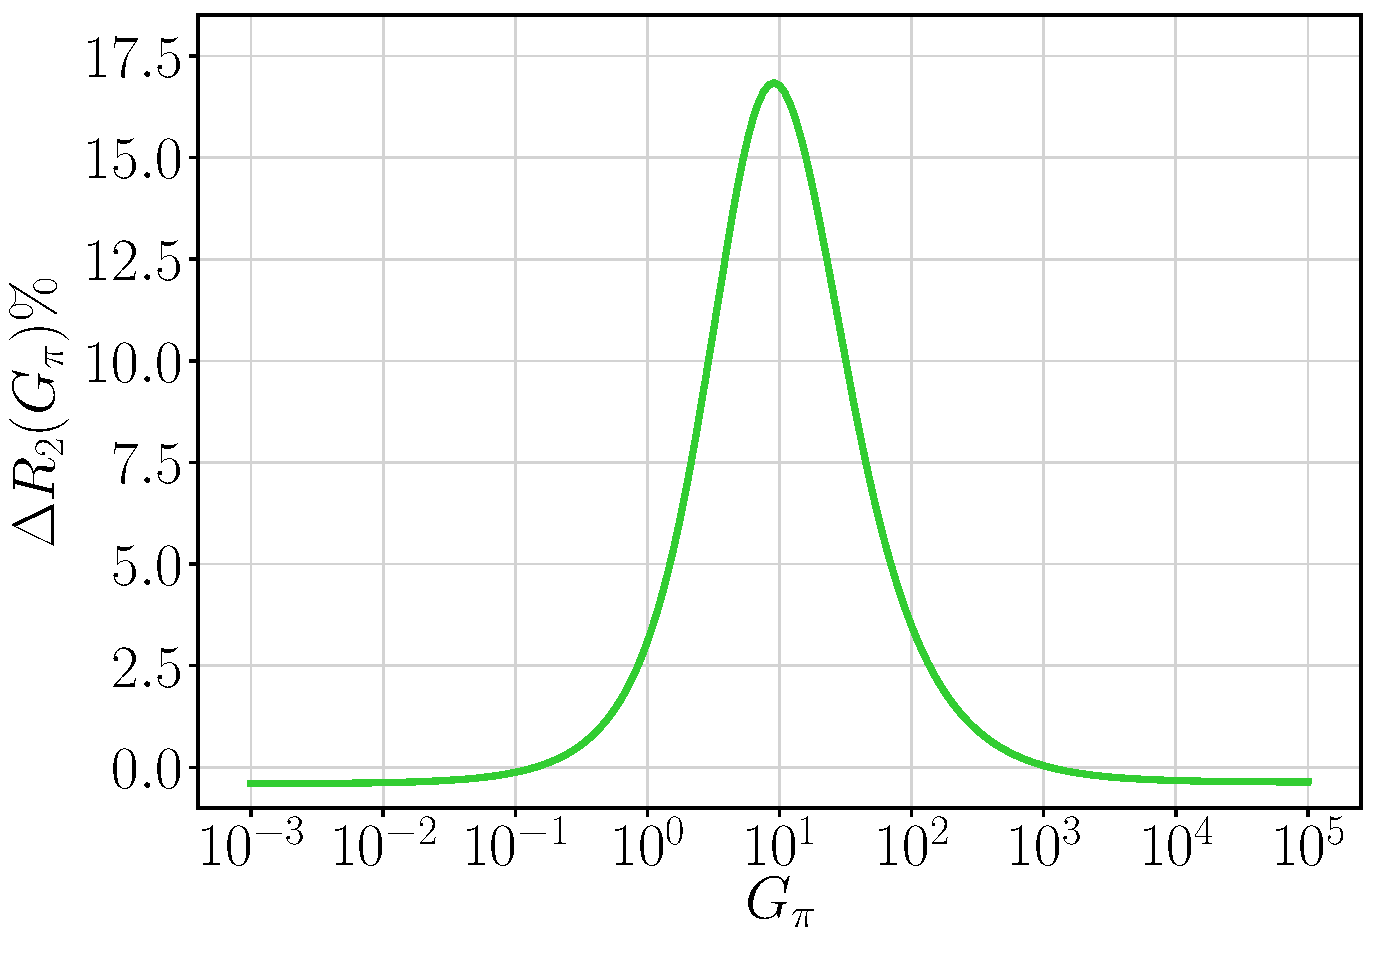
\includegraphics[width=.8\linewidth]{Figures/chapter05/G2-logerr}
		\end{minipage} \\[-1em]
		\begin{center}
			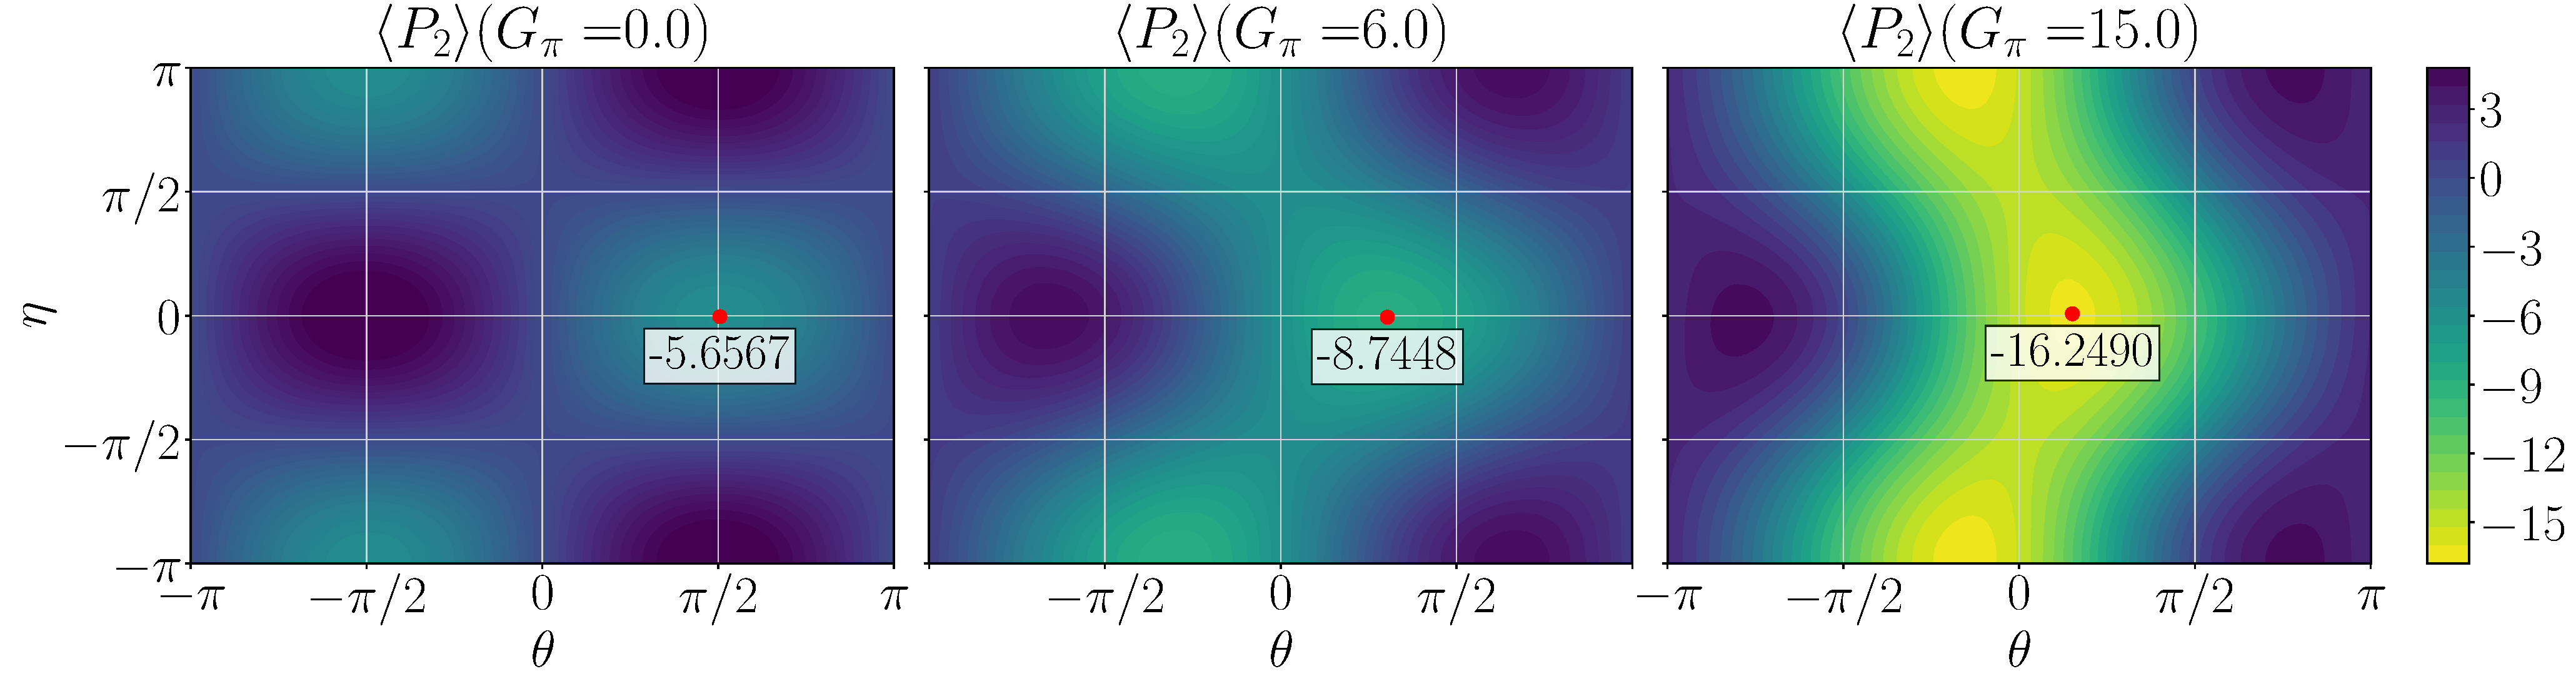
\includegraphics[width=.7\paperwidth]{Figures/chapter05/P2-tri-contour}
		\end{center}
		% \caption{Percentual error of the ground state energy results obtained from our quantum simulation with respect to the analytical solution and for different values of the coupling constant. (Left) Linear scale. (Right) Logarithmic scale.}
	\end{figure}
	\vspace{-2em}

\end{frame}



%% ----------------------------------------------------------------------------

\end{document}
